
\documentclass[twoside, 12pt]{amsart}

% Font

\usepackage[T1]{fontenc}
\usepackage[lf]{Baskervaldx} % lining figures
\usepackage[bigdelims,vvarbb]{newtxmath} % math italic letters from Nimbus Roman
\usepackage[cal=boondoxo]{mathalfa} % mathcal from STIX, unslanted a bit
\renewcommand*\oldstylenums[1]{\textosf{#1}}

\usepackage{latexsym}
\usepackage{amssymb}
\usepackage{amsmath}
\usepackage{amsthm}
\usepackage{amscd}
\usepackage{graphicx}
\usepackage[all]{xy}
\usepackage{a4wide}
\usepackage{mathrsfs} % mathscr

\usepackage{enumitem}

\usepackage{caption}
\usepackage{subcaption}

\usepackage{multirow}
%\usepackage{color}
\usepackage[dvipsnames]{xcolor}
\usepackage[colorlinks,final,hyperindex]{hyperref}
\usepackage[noabbrev,capitalize]{cleveref}
\usepackage{tikz}
\usepackage{tikz-cd}
\tikzset{math3d/.style=
    {x= {(-0.353cm,-0.353cm)}, z={(0cm,1cm)},y={(1cm,0cm)}}}
\tikzset{JLL3d/.style=
    {x= {(0.4cm,-0.2cm)}, z={(0cm,1cm)},y={(-1cm,0cm)}}}
\tikzset{J4/.style=
   {x= {(-0.87cm,-0.5cm)}, z={(0cm,1cm)},y={(0.87cm,-0.5cm)}}}

%MARGINS

\setlength{\textwidth}{\paperwidth}
\addtolength{\textwidth}{-2.5in}
\calclayout

% COLORS

\definecolor{Chocolat}{rgb}{0.36, 0.2, 0.09}
\definecolor{BleuTresFonce}{rgb}{0.215, 0.215, 0.36}
\definecolor{RougeTresFonce}{rgb}{0.36, 0.215, 0.215}
\hypersetup{citecolor=BleuTresFonce, linkcolor=black}

%%%%%%%% ENVIRONNEMENTS 

\newtheorem{definition}{Definition}[section]
\newtheorem{proposition}[definition]{Proposition}
\newtheorem{theorem}{Theorem}
\newtheorem*{problem}{Problem}
\newtheorem{corollary}{Corollary}

\newtheorem{lemma}[definition]{Lemma}
\newtheorem{conjecture}{Conjecture}

\theoremstyle{remark}
\newtheorem{example}[definition]{\sc Example}
\newtheorem{remark}[definition]{\sc Remark}

%%%%%%%%%%     NEW COMMANDS

\newcommand{\RR}{\mathbb{R}}
\newcommand{\ZZ}{\mathbb{Z}}
\newcommand{\ZP}{\mathbb{Z}_{>0}}
\newcommand{\K}{\mathrm{K}}
\newcommand{\J}{\mathrm{J}}
\newcommand{\La}{\mathcal{L}}
\newcommand{\Tam}[1]{\mathrm{PBT}_{#1}}
\newcommand{\PT}[1]{\mathrm{PT}_{#1}}
\newcommand{\CT}[1]{\mathrm{CT}_{#1}}
\newcommand{\CMT}[1]{\mathrm{CMT}_{#1}}
\newcommand{\sC}{\mathcal{C}}
\newcommand{\PolySub}{\mathsf{Poly}}
\renewcommand{\Top}{\mathsf{Top}}
\newcommand{\CW}{\mathsf{CW}}
\newcommand{\sF}{\mathcal{F}}
\DeclareMathOperator{\tp}{top}
\DeclareMathOperator{\bm}{bot}
\DeclareMathOperator{\pr}{pr}
\DeclareMathOperator{\conv}{conv}
\DeclareMathOperator{\diam}{diam}
\newcommand{\ang}[1]{\langle #1\rangle}
\newcommand{\No}{\mathcal{N}}
\newcommand{\Ve}{\mathcal{V}}
\newcommand{\Bool}[1]{\{0, 1\}^{#1}}
\newcommand{\sk}{\mathrm{sk}}
\DeclareMathOperator{\vol}{vol}
\newcommand{\tr}{\mathrm{tr}}
\newcommand{\id}{\mathrm{id}}
\newcommand{\itd}[1]{\triangle^{(#1)}}
\DeclareMathOperator*{\colim}{\mathrm{colim}}
\DeclareMathOperator{\im}{\mathrm{Im}}
\newcommand{\abs}[1]{\lvert #1\rvert}
\DeclareMathOperator{\codim}{codim}
\newcommand{\B}{\mathrm{B}}
\newcommand{\T}{\mathrm{T}}
\newcommand{\iBT}{\mathrm{i}^\T_\B}
\newcommand{\cat}[1]{\mathcal{#1}}
\newcommand{\gra}{\ell}
\newcommand{\Ainf}{\ensuremath{\mathrm{A}_\infty}}
\newcommand{\Linf}{\ensuremath{\mathrm{L}_\infty}}
\newcommand{\Ainfdeux}{\ensuremath{\mathrm{A}_\infty^2}}
\newcommand{\uAinf}{\ensuremath{\mathrm{uA}_\infty}}%A-infinity
\newcommand{\AAinf}{\mathrm{AA}_\infty} %AA-infinity
\newcommand{\Minf}{\ensuremath{\mathrm{M}_\infty}} %A-infinity bimodule
\newcommand{\Aalg}{\ensuremath{\mathrm{A}_\infty\text{-\hspace{2pt}}\mathsf{alg}}} %category A-infinity
\newcommand{\Acog}{\ensuremath{\mathrm{A}_\infty\text{-\hspace{2pt}}\mathsf{cog}}} %category A-infinity cog
\newcommand{\infAalg}{\ensuremath{\infty\text{-}\mathrm{A}_\infty\text{-}\mathsf{alg}}} %category A-infinity with morphisms
\newcommand{\infAcog}{\ensuremath{\infty\text{-}\mathrm{A}_\infty\text{-}\mathsf{cog}}} %category A-infinity with morphisms
\newcommand{\ide}{\ensuremath{\mathrm{id}}}
\newcommand{\mono}{\ensuremath{\mathrm{mono}}}
\newcommand{\comp}{\ensuremath{\mathrm{comp}}}
\newcommand{\ombas}{\ensuremath{\Omega B As}}
\newcommand{\diagainf}{\ensuremath{\triangle^{K}}}
\newcommand{\diagminf}{\ensuremath{\triangle^{J}}}

%OEIS
\newcommand{\OEIS}[1]{{\rm \href{http://oeis.org/#1}{\texttt{#1}}}}

%Mots parentheses colores
\newcommand{\black}[1]{\boldsymbol{\left(\right.} #1 \boldsymbol{\left.\right)}}
\newcommand{\blue}[1]{\textcolor{MidnightBlue}{\boldsymbol{\left(\right.}} #1 \textcolor{MidnightBlue}{\boldsymbol{\left.\right)}}} 
\newcommand{\red}[1]{\textcolor{BrickRed}{\boldsymbol{\left(\right.}} #1 \textcolor{BrickRed}{\boldsymbol{\left.\right)}}} 
\newcommand{\purple}[1]{\textcolor{Purple}{\boldsymbol{\left(\right.}} #1 \textcolor{Purple}{\boldsymbol{\left.\right)}}} 
\newcommand{\yellow}[1]{\textcolor{Dandelion}{\boldsymbol{\left(\right.}} #1 \textcolor{Dandelion}{\boldsymbol{\left.\right)}}} 
\newcommand{\green}[1]{\textcolor{ForestGreen}{\boldsymbol{\left(\right.}} #1 \textcolor{ForestGreen}{\boldsymbol{\left.\right)}}}
\newcommand{\orange}[1]{\textcolor{BurntOrange}{\boldsymbol{\left(\right.}} #1 \textcolor{BurntOrange}{\boldsymbol{\left.\right)}}} 

%textes colorés
\newcommand{\rouge}[1]{\textcolor{red}{#1}}

%%%% Trees NEW

\newcommand{\pointbullet}{

\begin{tikzpicture}[very thick]
\draw[fill,black] (0,0) circle (0.5) ;
\end{tikzpicture}}

\newcommand{\TreeLa}
{\vcenter{\hbox{
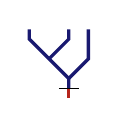
\begin{tikzpicture}[scale=0.25]
\draw[very thick, MidnightBlue] (0,-0.5)--(0,0) -- (-2,2)--(-2,2.5);
\draw[very thick, MidnightBlue] (-1,1)--(0,2)--(0,2.5) ;
\draw[very thick, MidnightBlue] (0,0)--(1,1)--(1,2.5) ;
%
\draw[very thick, BrickRed] (0,-0.5)--(0,-1) ;
%
\draw (-0.5,-0.5) --(0.5, -0.5);
\end{tikzpicture}}}}

\newcommand{\TreeLb}
{\vcenter{\hbox{

\begin{tikzpicture}[scale=0.25]
\draw[very thick, MidnightBlue] (-0.5,0.5)--(-2,2)--(-2,2.5);
\draw[very thick, MidnightBlue] (-1,1)--(0,2)--(0,2.5) ;
\draw[very thick, MidnightBlue] (0.5,0.5)--(1,1)--(1,2.5) ;
%
\draw[very thick, BrickRed] (0,0)--(0,-0.5) ;
\draw[very thick, BrickRed] (0,0)--(-0.5, 0.5) ;
\draw[very thick, BrickRed] (0,0)--(0.5,0.5) ;
%
\draw (-1,0.5) --(1, 0.5);
\end{tikzpicture}}}}

\newcommand{\TreeLc}
{\vcenter{\hbox{
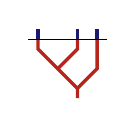
\begin{tikzpicture}[scale=0.25]
\draw[very thick, MidnightBlue] (-2, 2.5)--(-2, 3) ;
\draw[very thick, MidnightBlue] (0, 2.5)--(0, 3) ;
\draw[very thick, MidnightBlue] (1, 2.5)--(1, 3) ;
%
\draw[very thick, BrickRed] (0,-0.5)--(0,0) -- (-2,2)--(-2,2.5);
\draw[very thick, BrickRed] (-1,1)--(0,2)--(0,2.5) ;
\draw[very thick, BrickRed] (0,0)--(1,1)--(1,2.5) ;
%
\draw (-2.5,2.5) --(1.5, 2.5);
\end{tikzpicture}}}}

\newcommand{\TreeRa}
{\vcenter{\hbox{
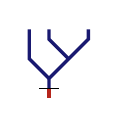
\begin{tikzpicture}[scale=0.25]
\draw[very thick, MidnightBlue] (0,-0.5)--(0,0) -- (2,2)--(2,2.5);
\draw[very thick, MidnightBlue] (1,1)--(0,2)--(0,2.5) ;
\draw[very thick, MidnightBlue] (0,0)--(-1,1)--(-1,2.5) ;
%
\draw[very thick, BrickRed] (0,-0.5)--(0,-1) ;
%
\draw (-0.5,-0.5) --(0.5, -0.5);
\end{tikzpicture}}}}

\newcommand{\TreeRb}
{\vcenter{\hbox{
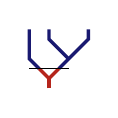
\begin{tikzpicture}[scale=0.25]
\draw[very thick, MidnightBlue] (0.5,0.5) -- (2,2)--(2,2.5);
\draw[very thick, MidnightBlue] (1,1)--(0,2)--(0,2.5) ;
\draw[very thick, MidnightBlue] (-0.5,0.5)--(-1,1)--(-1,2.5) ;
%
\draw[very thick, BrickRed] (0,-0.5)--(0,0) ;
\draw[very thick, BrickRed] (0,0)--(0.5,0.5) ;
\draw[very thick, BrickRed] (0,0)--(-0.5,0.5) ;
%
\draw (-1,0.5) --(1, 0.5);
\end{tikzpicture}}}}

\newcommand{\TreeRc}
{\vcenter{\hbox{
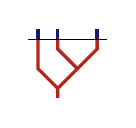
\begin{tikzpicture}[scale=0.25]
\draw[very thick, BrickRed] (0,-0.5)--(0,0) -- (2,2)--(2,2.5);
\draw[very thick, BrickRed] (1,1)--(0,2)--(0,2.5) ;
\draw[very thick, BrickRed] (0,0)--(-1,1)--(-1,2.5) ;
%
\draw[very thick, MidnightBlue] (2,2.5)--(2,3) ;
\draw[very thick, MidnightBlue] (0,2.5)--(0,3) ;
\draw[very thick, MidnightBlue] (-1,2.5)--(-1,3) ;
%
\draw (-1.5,2.5) --(2.5, 2.5);
\end{tikzpicture}}}}

\newcommand{\TreeLab}
{\vcenter{\hbox{
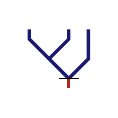
\begin{tikzpicture}[scale=0.25]
\draw[very thick, MidnightBlue] (0,0) -- (-2,2)--(-2,2.5);
\draw[very thick, MidnightBlue] (-1,1)--(0,2)--(0,2.5) ;
\draw[very thick, MidnightBlue] (0,0)--(1,1)--(1,2.5) ;
%
\draw[very thick, BrickRed] (0,0)--(0,-0.5) ;
%
\draw (-0.5,0) --(0.5, 0);
\end{tikzpicture}}}}

\newcommand{\TreeLbc}
{\vcenter{\hbox{
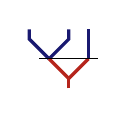
\begin{tikzpicture}[scale=0.25]
\draw[very thick, MidnightBlue] (-1,1) -- (-2,2)--(-2,2.5);
\draw[very thick, MidnightBlue] (-1,1)--(0,2)--(0,2.5) ;
\draw[very thick, MidnightBlue] (1,1)--(1,2.5) ;
%
\draw[very thick, BrickRed] (0,-0.5)--(0,0) ;
\draw[very thick, BrickRed] (0,0)--(-1,1) ;
\draw[very thick, BrickRed] (0,0)--(1,1) ;
%
\draw (-1.5,1) --(1.5, 1);
\end{tikzpicture}}}}

\newcommand{\TreeRab}
{\vcenter{\hbox{
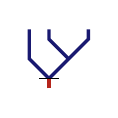
\begin{tikzpicture}[scale=0.25]
\draw[very thick, MidnightBlue] (0,0) -- (2,2)--(2,2.5);
\draw[very thick, MidnightBlue] (1,1)--(0,2)--(0,2.5) ;
\draw[very thick, MidnightBlue] (0,0)--(-1,1)--(-1,2.5) ;
%
\draw[very thick, BrickRed] (0,-0.5)--(0,0) ;
%
\draw (-0.5,0) --(0.5, 0);
\end{tikzpicture}}}}

\newcommand{\TreeRbc}
{\vcenter{\hbox{
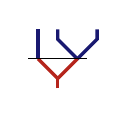
\begin{tikzpicture}[scale=0.25]
\draw[very thick, MidnightBlue] (1,1) -- (2,2)--(2,2.5);
\draw[very thick, MidnightBlue] (1,1)--(0,2)--(0,2.5) ;
\draw[very thick, MidnightBlue] (-1,1)--(-1,2.5) ;
%
\draw[very thick, BrickRed] (0,-0.5)--(0,0) ;
\draw[very thick, BrickRed] (0,0)--(1,1) ;
\draw[very thick, BrickRed] (0,0)--(-1,1) ;
%
\draw (-1.5,1) --(1.5, 1);
\end{tikzpicture}}}}

\newcommand{\TreeCa}
{\vcenter{\hbox{
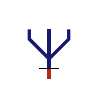
\begin{tikzpicture}[scale=0.25]
\draw[very thick, MidnightBlue] (0,-0.5) -- (0,1.5);
\draw[very thick, MidnightBlue] (0,0) -- (-1,1)--(-1,1.5);
\draw[very thick, MidnightBlue] (0,0) -- (1,1)--(1,1.5);
%
\draw[very thick, BrickRed] (0,-0.5)--(0,-1) ;
%
\draw (-0.5,-0.5) --(0.5, -0.5);
\end{tikzpicture}}}}

\newcommand{\TreeCb}
{\vcenter{\hbox{
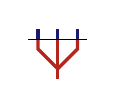
\begin{tikzpicture}[scale=0.25]
\draw[very thick, BrickRed] (0,-0.5) -- (0,1.5);
\draw[very thick, BrickRed] (0,0) -- (-1,1)--(-1,1.5);
\draw[very thick, BrickRed] (0,0) -- (1,1)--(1,1.5);
%
\draw[very thick, MidnightBlue] (-1,1.5)--(-1,2) ;
\draw[very thick, MidnightBlue] (0,1.5)--(0,2) ;
\draw[very thick, MidnightBlue] (1,1.5)--(1,2) ;
%
\draw (-1.5,1.5) --(1.5, 1.5);
\end{tikzpicture}}}}

\newcommand{\TreeCab}
{\vcenter{\hbox{

\begin{tikzpicture}[scale=0.25]
\draw[very thick, MidnightBlue] (0,0) -- (0,1.5);
\draw[very thick, MidnightBlue] (0,0) -- (-1,1)--(-1,1.5);
\draw[very thick, MidnightBlue] (0,0) -- (1,1)--(1,1.5);
%
\draw[very thick, BrickRed] (0,-0.5)--(0,0) ;
%
\draw (-0.5,0) --(0.5, 0);
\end{tikzpicture}}}}

\newcommand{\TreeIab}
{\vcenter{\hbox{
\begin{tikzpicture}[scale=0.35]
\draw[very thick, MidnightBlue] (0,0.5)--(0,0);
%
\draw[very thick, BrickRed] (0,-0.5)--(0,0) ;
%
\draw (-0.25,0) --(0.25, 0);
\end{tikzpicture}}}}

\newcommand{\TreeBa}
{\vcenter{\hbox{
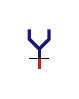
\begin{tikzpicture}[scale=0.25]
\draw[very thick, MidnightBlue] (0,0.5)--(0,1);
\draw[very thick, MidnightBlue] (0,1)--(-0.5,1.5)--(-0.5,2);
\draw[very thick, MidnightBlue] (0,1)--(0.5,1.5)--(0.5,2);
% 
\draw[very thick, BrickRed] (0,0)--(0,0.5);
\draw (-0.5,0.5) --(0.5, 0.5);\end{tikzpicture}}}}

\newcommand{\TreeBb}
{\vcenter{\hbox{
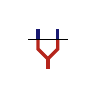
\begin{tikzpicture}[scale=0.25]
\draw[very thick, MidnightBlue] (-0.5,2)--(-0.5,2.5);
\draw[very thick, MidnightBlue] (0.5,2)--(0.5,2.5);
%
\draw[very thick, BrickRed] (0,0.5)--(0,1);
\draw[very thick, BrickRed] (0,1)--(-0.5,1.5)--(-0.5,2);
\draw[very thick, BrickRed] (0,1)--(0.5,1.5)--(0.5,2);
% 
\draw (-1,2) --(1, 2);
\end{tikzpicture}}}}

\newcommand{\TreeBab}
{\vcenter{\hbox{

\begin{tikzpicture}[scale=0.25]
\draw[very thick, MidnightBlue] (0,1)--(-0.5,1.5)--(-0.5,2);
\draw[very thick, MidnightBlue] (0,1)--(0.5,1.5)--(0.5,2);
% 
\draw[very thick, BrickRed] (0,0.5)--(0,1);
\draw (-0.5,1) --(0.5,1);
\end{tikzpicture}}}}

%%%% Trees OLD

\newcommand{\TreeR}
{\vcenter{\hbox{
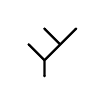
\begin{tikzpicture}[yscale=0.2,xscale=0.2]
\draw[thick] (0,-1)--(0,0) -- (2,2);
\draw[thick] (1,1)--(0,2) ;
\draw[thick] (0,0)--(-1,1) ;
\draw [fill] (0,-1) circle [radius=0.035];
\draw [fill] (2,2) circle [radius=0.035];
\draw [fill] (0,2) circle [radius=0.035];
\draw [fill] (-1,1) circle [radius=0.035];
\end{tikzpicture}}}}
\newcommand{\TreeL}
{\vcenter{\hbox{
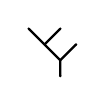
\begin{tikzpicture}[yscale=0.2,xscale=0.2]
\draw[thick] (0,-1)--(0,0) -- (-2,2);
\draw[thick] (-1,1)--(0,2) ;
\draw[thick] (0,0)--(1,1) ;
\draw [fill] (0,-1) circle [radius=0.035];
\draw [fill] (-2,2) circle [radius=0.035];
\draw [fill] (0,2) circle [radius=0.035];
\draw [fill] (1,1) circle [radius=0.035];
\end{tikzpicture}}}}
\newcommand{\TreeLL}
{\vcenter{\hbox{
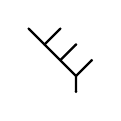
\begin{tikzpicture}[yscale=0.2,xscale=0.2]
\draw[thick] (0,-1)--(0,0) -- (-3,3);
\draw[thick] (-1,1)--(0,2) ;
\draw[thick] (-2,2)--(-1,3) ;
\draw[thick] (0,0)--(1,1) ;
\draw [fill] (0,-1) circle [radius=0.035];
\draw [fill] (-2,2) circle [radius=0.035];
\draw [fill] (0,2) circle [radius=0.035];
\draw [fill] (1,1) circle [radius=0.035];
\draw [fill] (-3,3) circle [radius=0.035];
\draw [fill] (-1,3) circle [radius=0.035];
\end{tikzpicture}}}}
\newcommand{\TreeLR}
{\vcenter{\hbox{
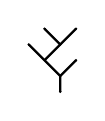
\begin{tikzpicture}[yscale=0.2,xscale=0.2]
\draw[thick] (0,-1)--(0,0) -- (-2,2);
\draw[thick] (-1,1)--(1,3) ;
\draw[thick] (0,0)--(1,1) ;
\draw[thick] (0,2)--(-1,3) ;
\draw [fill] (0,-1) circle [radius=0.035];
\draw [fill] (-2,2) circle [radius=0.035];
\draw [fill] (0,2) circle [radius=0.035];
\draw [fill] (1,1) circle [radius=0.035];
\draw [fill] (-1,3) circle [radius=0.035];
\draw [fill] (1,3) circle [radius=0.035];
\end{tikzpicture}}}}
\newcommand{\TreeRR}
{\vcenter{\hbox{
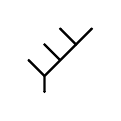
\begin{tikzpicture}[yscale=0.2,xscale=0.2]
\draw[thick] (0,-1)--(0,0) -- (3,3);
\draw[thick] (1,1)--(0,2) ;
\draw[thick] (2,2)--(1,3) ;
\draw[thick] (0,0)--(-1,1) ;
\draw [fill] (0,-1) circle [radius=0.035];
\draw [fill] (2,2) circle [radius=0.035];
\draw [fill] (0,2) circle [radius=0.035];
\draw [fill] (-1,1) circle [radius=0.035];
\draw [fill] (3,3) circle [radius=0.035];
\draw [fill] (1,3) circle [radius=0.035];
\end{tikzpicture}}}}
\newcommand{\TreeRL}
{\vcenter{\hbox{
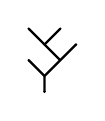
\begin{tikzpicture}[yscale=0.2,xscale=0.2]
\draw[thick] (0,-1)--(0,0) -- (2,2);
\draw[thick] (1,1)--(-1,3) ;
\draw[thick] (0,0)--(-1,1) ;
\draw[thick] (0,2)--(1,3) ;
\draw [fill] (0,-1) circle [radius=0.035];
\draw [fill] (2,2) circle [radius=0.035];
\draw [fill] (0,2) circle [radius=0.035];
\draw [fill] (-1,1) circle [radius=0.035];
\draw [fill] (1,3) circle [radius=0.035];
\draw [fill] (-1,3) circle [radius=0.035];
\end{tikzpicture}}}}
\newcommand{\TreeCC}
{\vcenter{\hbox{
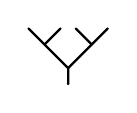
\begin{tikzpicture}[yscale=0.2,xscale=0.2]
\draw[thick] (0,-1)--(0,0) -- (-2.5,2.5);
\draw[thick] (-1.5,1.5)--(-0.5,2.5) ;
\draw[thick] (1.5,1.5)--(0.5,2.5) ;
\draw[thick] (0,0)--(2.5,2.5) ;
\draw [fill] (0,-1) circle [radius=0.035];
\draw [fill] (-2.5,2.5) circle [radius=0.035];
\draw [fill] (-0.5,2.5) circle [radius=0.035];
\draw [fill] (0.5,2.5) circle [radius=0.035];
\draw [fill] (2.5,2.5) circle [radius=0.035];
\end{tikzpicture}}}}
\newcommand{\TreeAL}
{\vcenter{\hbox{
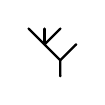
\begin{tikzpicture}[yscale=0.2,xscale=0.2]
\draw[thick] (0,-1)--(0,0) -- (-2,2);
\draw[thick] (-1,1)--(0,2) ;
\draw[thick] (0,0)--(1,1) ;
\draw[thick] (-1,1)--(-1,2) ;
\draw [fill] (0,-1) circle [radius=0.035];
\draw [fill] (-2,2) circle [radius=0.035];
\draw [fill] (0,2) circle [radius=0.035];
\draw [fill] (1,1) circle [radius=0.035];
\draw [fill] (-1,2) circle [radius=0.035];
\end{tikzpicture}}}}
\newcommand{\TreeRA}
{\vcenter{\hbox{
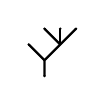
\begin{tikzpicture}[yscale=0.2,xscale=0.2]
\draw[thick] (0,-1)--(0,0) -- (2,2);
\draw[thick] (1,1)--(0,2) ;
\draw[thick] (0,0)--(-1,1) ;
\draw[thick] (1,1)--(1,2) ;
\draw [fill] (0,-1) circle [radius=0.035];
\draw [fill] (2,2) circle [radius=0.035];
\draw [fill] (0,2) circle [radius=0.035];
\draw [fill] (-1,1) circle [radius=0.035];
\draw [fill] (1,2) circle [radius=0.035];
\end{tikzpicture}}}}
\newcommand{\TreeAR}
{\vcenter{\hbox{
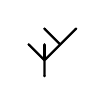
\begin{tikzpicture}[yscale=0.2,xscale=0.2]
\draw[thick] (0,-1)--(0,0) -- (2,2);
\draw[thick] (1,1)--(0,2) ;
\draw[thick] (0,0)--(-1,1) ;
\draw[thick] (0,0)--(0,1) ;
\draw [fill] (0,-1) circle [radius=0.035];
\draw [fill] (2,2) circle [radius=0.035];
\draw [fill] (0,2) circle [radius=0.035];
\draw [fill] (-1,1) circle [radius=0.035];
\draw [fill] (0,1) circle [radius=0.035];
\end{tikzpicture}}}}
\newcommand{\TreeLA}
{\vcenter{\hbox{
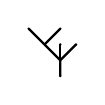
\begin{tikzpicture}[yscale=0.2,xscale=0.2]
\draw[thick] (0,-1)--(0,0) -- (-2,2);
\draw[thick] (-1,1)--(0,2) ;
\draw[thick] (0,0)--(1,1) ;
\draw[thick] (0,0)--(0,1) ;
\draw [fill] (0,-1) circle [radius=0.035];
\draw [fill] (-2,2) circle [radius=0.035];
\draw [fill] (0,2) circle [radius=0.035];
\draw [fill] (1,1) circle [radius=0.035];
\draw [fill] (0,1) circle [radius=0.035];
\end{tikzpicture}}}}
\newcommand{\TreeCA}
{\vcenter{\hbox{
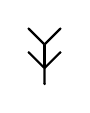
\begin{tikzpicture}[yscale=0.2,xscale=0.2]
\draw[thick] (0,-1)--(0,0) -- (-1,1);
\draw[thick] (0,1.5)--(1,2.5) ;
\draw[thick] (0,1.5)--(-1,2.5) ;
\draw[thick] (0,0)--(1,1) ;
\draw[thick] (0,0)--(0,1.5) ;
\draw [fill] (0,-1) circle [radius=0.035];
\draw [fill] (-1,1) circle [radius=0.035];
\draw [fill] (1,2.5) circle [radius=0.035];
\draw [fill] (-1,2.5) circle [radius=0.035];
\draw [fill] (1,1) circle [radius=0.035];
\draw [fill] (0,1) circle [radius=0.035];
\end{tikzpicture}}}}
\newcommand{\TreeC}
{\vcenter{\hbox{
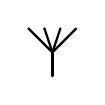
\begin{tikzpicture}[yscale=0.2,xscale=0.2]
\draw[thick] (0,-1.5)--(0,0);
\draw[thick] (0,0)--(1.5,1.5) ;
\draw[thick] (0,0)--(0.5,1.5) ;
\draw[thick] (0,0)--(-0.5,1.5) ;
\draw[thick] (0,0)--(-1.5,1.5) ;
\draw [fill] (0,-1.5) circle [radius=0.035];
\draw [fill] (1.5,1.5) circle [radius=0.035];
\draw [fill] (0.5,1.5) circle [radius=0.035];
\draw [fill] (-1.5,1.5) circle [radius=0.035];
\draw [fill] (-0.5,1.5) circle [radius=0.035];
\end{tikzpicture}}}}

%Drapeau européen

\usepackage{graphicx,calc}
\newlength\myheight
\newlength\mydepth
\settototalheight\myheight{Xygp}
\settodepth\mydepth{Xygp}
\setlength\fboxsep{0pt}
\newcommand*\inlinegraphics[1]{%
  \settototalheight\myheight{Xygp}%
  \settodepth\mydepth{Xygp}%
  \raisebox{-\mydepth}{\includegraphics[height=\myheight]{#1}}%
}

%%%%%%%%% Nouveau

\DeclareMathOperator{\Ima}{Im} %Image d'une fonction
\DeclareMathOperator{\cone}{Cone} %Cône

%%%%%%%%%%%   Comments 

\newcommand{\Thibaut}[1]{\textcolor{red}{#1}}
\newcommand{\Guillaume}[1]{\textcolor{blue}{#1}}
\newcommand{\End}{\ensuremath{\mathrm{End}}}
\newcommand{\coEnd}{\ensuremath{\mathrm{coEnd}}}
\newcommand{\Hom}{\ensuremath{\mathrm{Hom}}}

\newcommand{\arbreoptrois}{
\begin{tikzpicture}[scale=0.15,baseline=(pt_base.base)]

\coordinate (pt_base) at (0,-0.5) ;

\draw (0,1.25) -- (0,0) ;
\draw (-1.25,1.25) -- (0,0) ;
\draw (1.25,1.25) -- (0,0) ;
\draw (0,-1.25) -- (0,0) ;

\end{tikzpicture}
}

\newcommand{\premiertermecobarbarA}{
\begin{tikzpicture}[scale=0.15,baseline=(pt_base.base)]

\coordinate (pt_base) at (0,-0.5) ;

\draw (-1.25,1.25) -- (0,0) ;
\draw (1.25,1.25) -- (0,0) ;
\draw (0,-1.25) -- (0,0) ;

\end{tikzpicture}
}

\newcommand{\premiertermecobarbarAprime}{
\begin{tikzpicture}[scale=0.07,baseline=(pt_base.base)]

\coordinate (pt_base) at (0,-0.5) ;

\draw (-1.25,1.25) -- (0,0) ;
\draw (1.25,1.25) -- (0,0) ;
\draw (0,-1.25) -- (0,0) ;

\end{tikzpicture}
}

\newcommand{\premiertermecobarbarB}{
\begin{tikzpicture}[scale = 0.15,baseline = (O.base)]
\node (K) at (-0.625,0.625) {} ;
\node (L) at (0,0) {} ;
\draw (-0.625,0.625) -- (0,1.25) ;
\draw (-1.25,1.25) -- (0,0) ;
\draw (1.25,1.25) -- (0,0) ;
\draw (0,-1.25) -- (0,0) ;
\node (O) at (0,-0.5) {} ;
\end{tikzpicture}
}

\newcommand{\premiertermecobarbarC}{
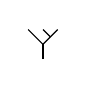
\begin{tikzpicture}[scale = 0.15,baseline = (O.base)]
\node (K) at (0.625,0.625) {} ;
\node (L) at (0,0) {} ;
\draw (0.625,0.625) -- (0,1.25) ;
\draw (-1.25,1.25) -- (0,0) ;
\draw (1.25,1.25) -- (0,0) ;
\draw (0,-1.25) -- (0,0) ;
\node (O) at (0,-0.5) {} ;
\end{tikzpicture}
}

\newcommand{\premiertermecobarbarD}{
\begin{tikzpicture}[scale=0.15,baseline=(pt_base.base)]

\coordinate (pt_base) at (0,-0.5) ;

\draw (0,1.25) -- (0,0) ;
\draw (-1.25,1.25) -- (0,0) ;
\draw (1.25,1.25) -- (0,0) ;
\draw (0,-1.25) -- (0,0) ;

\end{tikzpicture}
}

\newcommand{\arbreopdeuxcol}[1]{
\begin{tikzpicture}[scale=0.15,baseline=(pt_base.base)]

\coordinate (pt_base) at (0,-0.5) ;

\draw[#1] (-1.25,1.25) -- (0,0) ;
\draw[#1] (1.25,1.25) -- (0,0) ;
\draw[#1] (0,-1.25) -- (0,0) ;

\end{tikzpicture}
}

% Opération ternaire colorée de l'opérade A-infini

\newcommand{\arbreoptroiscol}[1]{
\begin{tikzpicture}[scale=0.15,baseline=(pt_base.base)]

\coordinate (pt_base) at (0,-0.5) ;

\draw[#1] (0,1.25) -- (0,0) ;
\draw[#1] (-1.25,1.25) -- (0,0) ;
\draw[#1] (1.25,1.25) -- (0,0) ;
\draw[#1] (0,-1.25) -- (0,0) ;

\end{tikzpicture}
}

\usetikzlibrary{decorations.pathreplacing,calligraphy}
\usetikzlibrary{decorations.pathmorphing}

\newcommand{\compositionlabelIJ}{
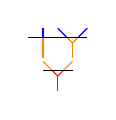
\begin{tikzpicture}[scale=0.15,baseline=(pt_base.base)]

\coordinate (pt_base) at (0,-0.5) ;

\draw[orange] (-1.25,1.25) -- (-0.5,0.5) ;
\draw[orange] (1.25,1.25) -- (0.5,0.5) ;

\draw[red] (-0.5,0.5) -- (0,0) ;
\draw[red] (0.5,0.5) -- (0,0) ;
\draw[red] (0,-1.25) -- (0,0) ;

\draw (-1.25,0.5) -- (1.25,0.5) ;

\begin{scope}[xshift=1.25cm,yshift=2.8cm]

\draw[blue] (-1.25,1.25) -- (-0.5,0.5) ;
\draw[blue] (1.25,1.25) -- (0.5,0.5) ;

\draw[orange] (-0.5,0.5) -- (0,0) ;
\draw[orange] (0.5,0.5) -- (0,0) ;
\draw[orange] (0,-1.25) -- (0,0) ;

\draw (-1.25,0.5) -- (1.25,0.5) ;

\end{scope}

\begin{scope}[xshift=-1.25cm,yshift=2.8cm]

\draw[blue] (0,1.25) -- (0,0.5) ;
\draw[orange] (0,-1.25) -- (0,0.5) ;

\draw (-1.25,0.5) -- (1.25,0.5) ;

\end{scope}

\end{tikzpicture}
}

\newcommand{\compositionlabelKL}{
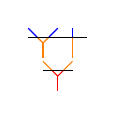
\begin{tikzpicture}[scale=0.15,baseline=(pt_base.base)]

\coordinate (pt_base) at (0,-0.5) ;

\draw[orange] (-1.25,1.25) -- (-0.5,0.5) ;
\draw[orange] (1.25,1.25) -- (0.5,0.5) ;

\draw[red] (-0.5,0.5) -- (0,0) ;
\draw[red] (0.5,0.5) -- (0,0) ;
\draw[red] (0,-1.25) -- (0,0) ;

\draw (-1.25,0.5) -- (1.25,0.5) ;

\begin{scope}[xshift=-1.25cm,yshift=2.8cm]

\draw[blue] (-1.25,1.25) -- (-0.5,0.5) ;
\draw[blue] (1.25,1.25) -- (0.5,0.5) ;

\draw[orange] (-0.5,0.5) -- (0,0) ;
\draw[orange] (0.5,0.5) -- (0,0) ;
\draw[orange] (0,-1.25) -- (0,0) ;

\draw (-1.25,0.5) -- (1.25,0.5) ;

\end{scope}

\begin{scope}[xshift=1.25cm,yshift=2.8cm]

\draw[blue] (0,1.25) -- (0,0.5) ;
\draw[orange] (0,-1.25) -- (0,0.5) ;

\draw (-1.25,0.5) -- (1.25,0.5) ;

\end{scope}

\end{tikzpicture}
}

\newcommand{\compositionlabelJK}{
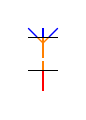
\begin{tikzpicture}[scale=0.15,baseline=(pt_base.base)]

\coordinate (pt_base) at (0,-0.5) ;

\draw[blue] (0,1.25) -- (0,0.5) ;
\draw[blue] (-1.25,1.25) -- (-0.5,0.5) ;
\draw[blue] (1.25,1.25) -- (0.5,0.5) ;

\draw[orange] (0,0.5) -- (0,0) ;
\draw[orange] (-0.5,0.5) -- (0,0) ;
\draw[orange] (0.5,0.5) -- (0,0) ;
\draw[orange] (0,-1.25) -- (0,0) ;

\draw (-1.25,0.5) -- (1.25,0.5) ;

\begin{scope}[yshift = -2.8cm ]

\draw[orange] (0,1.25) -- (0,0.5) ;
\draw[red] (0,-1.25) -- (0,0.5) ;

\draw (-1.25,0.5) -- (1.25,0.5) ;

\end{scope}

\end{tikzpicture}
}

\newcommand{\compositionlabelIL}{
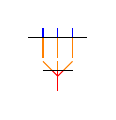
\begin{tikzpicture}[scale=0.15,baseline=(pt_base.base)]

\coordinate (pt_base) at (0,-0.5) ;

\draw[orange] (0,1.25) -- (0,0.5) ;
\draw[orange] (-1.25,1.25) -- (-0.5,0.5) ;
\draw[orange] (1.25,1.25) -- (0.5,0.5) ;

\draw[red] (0,0.5) -- (0,0) ;
\draw[red] (-0.5,0.5) -- (0,0) ;
\draw[red] (0.5,0.5) -- (0,0) ;
\draw[red] (0,-1.25) -- (0,0) ;

\draw (-1.25,0.5) -- (1.25,0.5) ;

\begin{scope}[yshift = 2.8cm ]

\draw[blue] (0,1.25) -- (0,0.5) ;
\draw[orange] (0,-1.25) -- (0,0.5) ;

\draw (-1.25,0.5) -- (1.25,0.5) ;

\end{scope}

\begin{scope}[xshift= -1.25cm, yshift = 2.8cm ]

\draw[blue] (0,1.25) -- (0,0.5) ;
\draw[orange] (0,-1.25) -- (0,0.5) ;

\draw (-1.25,0.5) -- (1.25,0.5) ;

\end{scope}

\begin{scope}[xshift= 1.25cm, yshift = 2.8cm ]

\draw[blue] (0,1.25) -- (0,0.5) ;
\draw[orange] (0,-1.25) -- (0,0.5) ;

\draw (-1.25,0.5) -- (1.25,0.5) ;

\end{scope}

\end{tikzpicture}
}

% Opérations colorées de l'opérade A-infini

\newcommand{\arbreoprouge}[1]{
\begin{tikzpicture}[scale=#1,baseline=(pt_base.base)]

\coordinate (pt_base) at (0,-0.5) ;

\draw[red] (-2,1.25) -- (0,0) ;
\draw[red] (-1,1.25) -- (0,0) ;
\draw[red] (1,1.25) -- (0,0) ;
\draw[red] (2,1.25) -- (0,0) ;
\draw[red] (0,-1.25) -- (0,0) ;

\draw[red] [densely dotted] (-0.5,0.9) -- (0.5,0.9) ;

\end{tikzpicture}}

\newcommand{\arbreopbleu}[1]{
\begin{tikzpicture}[scale=#1,baseline=(pt_base.base)]

\coordinate (pt_base) at (0,-0.5) ;

\draw[blue] (-2,1.25) -- (0,0) ;
\draw[blue] (-1,1.25) -- (0,0) ;
\draw[blue] (1,1.25) -- (0,0) ;
\draw[blue] (2,1.25) -- (0,0) ;
\draw[blue] (0,-1.25) -- (0,0) ;

\draw[blue] [densely dotted] (-0.5,0.9) -- (0.5,0.9) ;

\end{tikzpicture}}

% Opérations du bimodule opéradique A-infini - Morph

\newcommand{\arbreopmorph}[1]{
\begin{tikzpicture}[scale=#1,baseline=(pt_base.base)]

\coordinate (pt_base) at (0,-0.5) ;

\draw[blue] (-2,1.25) -- (0,0) ;
\draw[blue] (-1,1.25) -- (0,0) ;
\draw[blue] (1,1.25) -- (0,0) ;
\draw[blue] (2,1.25) -- (0,0) ;

\draw[red] (0,-1.25) -- (0,0) ;

\draw[blue] [densely dotted] (-0.5,0.9) -- (0.5,0.9) ;

\draw  (-1.5,0) -- (1.5,0) ;

\end{tikzpicture}}

\newcommand{\arbreopmorphcompun}{
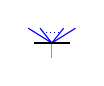
\begin{tikzpicture}[scale=0.15,baseline=(pt_base.base)]

\coordinate (pt_base) at (0,-0.5) ;

\draw[blue] (-2,1.25) -- (0,0) ;
\draw[blue] (-1,1.25) -- (0,0) ;
\draw[blue] (1,1.25) -- (0,0) ;
\draw[blue] (2,1.25) -- (0,0) ;

\draw[orange] (0,-1.25) -- (0,0) ;

\draw[blue] [densely dotted] (-0.5,0.9) -- (0.5,0.9) ;

\draw  (-1.5,0) -- (1.5,0) ;

\end{tikzpicture}}

\newcommand{\arbreopmorphcompdeux}{
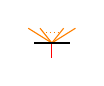
\begin{tikzpicture}[scale=0.15,baseline=(pt_base.base)]

\coordinate (pt_base) at (0,-0.5) ;

\draw[orange] (-2,1.25) -- (0,0) ;
\draw[orange] (-1,1.25) -- (0,0) ;
\draw[orange] (1,1.25) -- (0,0) ;
\draw[orange] (2,1.25) -- (0,0) ;

\draw[red] (0,-1.25) -- (0,0) ;

\draw[orange] [densely dotted] (-0.5,0.9) -- (0.5,0.9) ;

\draw  (-1.5,0) -- (1.5,0) ;

\end{tikzpicture}}

% Opération binaire de A-infini - Morph

\newcommand{\arbreopdeuxmorph}{
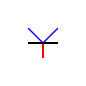
\begin{tikzpicture}[scale=0.15,baseline=(pt_base.base)]

\coordinate (pt_base) at (0,-0.5) ;

\draw[blue] (-1.25,1.25) -- (0,0) ;
\draw[blue] (1.25,1.25) -- (0,0) ;
\draw[red] (0,-1.25) -- (0,0) ;

\draw (-1.25,0) -- (1.25,0) ;

\end{tikzpicture}
}

\newcommand{\arbreopdeuxmorphcompun}{
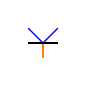
\begin{tikzpicture}[scale=0.15,baseline=(pt_base.base)]

\coordinate (pt_base) at (0,-0.5) ;

\draw[blue] (-1.25,1.25) -- (0,0) ;
\draw[blue] (1.25,1.25) -- (0,0) ;
\draw[orange] (0,-1.25) -- (0,0) ;

\draw (-1.25,0) -- (1.25,0) ;

\end{tikzpicture}
}

\newcommand{\arbreopdeuxmorphcompdeux}{
\begin{tikzpicture}[scale=0.15,baseline=(pt_base.base)]

\coordinate (pt_base) at (0,-0.5) ;

\draw[orange] (-1.25,1.25) -- (0,0) ;
\draw[orange] (1.25,1.25) -- (0,0) ;
\draw[red] (0,-1.25) -- (0,0) ;

\draw (-1.25,0) -- (1.25,0) ;

\end{tikzpicture}
}

\newcommand{\arbreopcompun}{
\begin{tikzpicture}[scale=0.15,baseline=(pt_base.base)]

\coordinate (pt_base) at (0,-2) ;

\draw[blue] (-1.25,1.25) -- (0,0) ;
\draw[blue] (1.25,1.25) -- (0,0) ;
\draw[orange] (0,-2.5) -- (0,0) ;
\draw[red] (0,-3.75) -- (0,-2.5) ;

\draw (-1.25,0) -- (1.25,0) ;

\draw (-1.25,-2.5) -- (1.25,-2.5) ;

\end{tikzpicture}
}

\newcommand{\arbreopcompdeux}{
\begin{tikzpicture}[scale=0.15,baseline=(pt_base.base)]

\coordinate (pt_base) at (0,0.5) ;

\draw[blue] (-1.25,3.75) -- (-1.25,2.5) ;
\draw[blue] (1.25,3.75) -- (1.25,2.5) ;
\draw[orange] (-1.25,1.25) -- (-1.25,2.5) ;
\draw[orange] (1.25,1.25) -- (1.25,2.5) ;
\draw[orange] (-1.25,1.25) -- (0,0) ;
\draw[orange] (1.25,1.25) -- (0,0) ;
\draw[red] (0,-1.25) -- (0,0) ;

\draw (-1.25,0) -- (1.25,0) ;
\draw (-1.75,2.5) -- (-0.75,2.5) ;
\draw (1.75,2.5) -- (0.75,2.5) ;

\end{tikzpicture}
}

% Opération ternaire de A-infini - Morph

\newcommand{\arbreoptroismorph}{
\begin{tikzpicture}[scale=0.15,baseline=(pt_base.base)]

\coordinate (pt_base) at (0,-0.5) ;

\draw[blue] (0,1.25) -- (0,0) ;
\draw[blue] (-1.25,1.25) -- (0,0) ;
\draw[blue] (1.25,1.25) -- (0,0) ;

\draw[red] (0,-1.25) -- (0,0) ;

\draw (-1.25,0) -- (1.25,0) ;

\end{tikzpicture}
}

\newcommand{\arbreoptroismorphcompun}{
\begin{tikzpicture}[scale=0.15,baseline=(pt_base.base)]

\coordinate (pt_base) at (0,-0.5) ;

\draw[blue] (0,1.25) -- (0,0) ;
\draw[blue] (-1.25,1.25) -- (0,0) ;
\draw[blue] (1.25,1.25) -- (0,0) ;

\draw[orange] (0,-1.25) -- (0,0) ;

\draw (-1.25,0) -- (1.25,0) ;

\end{tikzpicture}
}

\newcommand{\arbreoptroismorphcompdeux}{
\begin{tikzpicture}[scale=0.15,baseline=(pt_base.base)]

\coordinate (pt_base) at (0,-0.5) ;

\draw[orange] (0,1.25) -- (0,0) ;
\draw[orange] (-1.25,1.25) -- (0,0) ;
\draw[orange] (1.25,1.25) -- (0,0) ;

\draw[red] (0,-1.25) -- (0,0) ;

\draw (-1.25,0) -- (1.25,0) ;

\end{tikzpicture}
}

% Opération quaternaire de A-infini - Morph

\newcommand{\arbreopquatremorph}{
\begin{tikzpicture}[scale=0.15,baseline=(pt_base.base)]

\coordinate (pt_base) at (0,-0.5) ;

\draw[blue] (-1.5,1.25) -- (0,0) ;
\draw[blue] (1.5,1.25) -- (0,0) ;
\draw[blue] (-0.5,1.25) -- (0,0) ;
\draw[blue] (0.5,1.25) -- (0,0) ;

\draw[red] (0,-1.25) -- (0,0) ;

\draw (-1.5,0) -- (1.5,0) ;

\end{tikzpicture}
}

\newcommand{\arbreopquatremorphcompun}{
\begin{tikzpicture}[scale=0.15,baseline=(pt_base.base)]

\coordinate (pt_base) at (0,-0.5) ;

\draw[blue] (-1.5,1.25) -- (0,0) ;
\draw[blue] (1.5,1.25) -- (0,0) ;
\draw[blue] (-0.5,1.25) -- (0,0) ;
\draw[blue] (0.5,1.25) -- (0,0) ;

\draw[orange] (0,-1.25) -- (0,0) ;

\draw (-1.5,0) -- (1.5,0) ;

\end{tikzpicture}
}

\newcommand{\arbreopquatremorphcompdeux}{
\begin{tikzpicture}[scale=0.15,baseline=(pt_base.base)]

\coordinate (pt_base) at (0,-0.5) ;

\draw[orange] (-1.5,1.25) -- (0,0) ;
\draw[orange] (1.5,1.25) -- (0,0) ;
\draw[orange] (-0.5,1.25) -- (0,0) ;
\draw[orange] (0.5,1.25) -- (0,0) ;

\draw[red] (0,-1.25) -- (0,0) ;

\draw (-1.5,0) -- (1.5,0) ;

\end{tikzpicture}
}

% Compositions partielles de A-infini - Morph 1

\newcommand{\eqainfmorphun}{
\begin{tikzpicture}[scale=0.2,baseline=(pt_base.base)]

\coordinate (pt_base) at (0,1.25) ;

%étiquetages

\draw [decorate,    decoration = {calligraphic brace}] (-4,1.5) --  (-0.5,1.5) ;
\draw [decorate,    decoration = {calligraphic brace}] (0.5,1.5) --  (4,1.5) ;
\draw [decorate,    decoration = {calligraphic brace}] (-2,4) --  (2,4) ;

\node[above] at (-2.3,1.5) {\tiny $p$} ; 
\node[above] at (0,4) {\tiny $q$} ; 
\node[above] at (2.3,1.5) {\tiny $r$} ; 

% traits bicolorés

\draw[blue] (-4,1.25) -- (0,0) ;
\draw[blue] (-3,1.25) -- (0,0) ;
\draw[blue] (4,1.25) -- (0,0) ;
\draw[blue] (3,1.25) -- (0,0) ;
\draw[blue] (0,1.25) -- (0,0) ;

\draw[red] (0,-1.25) -- (0,0) ; 

% traits arbre supérieur

\draw[blue] (-2,3.75) -- (0,2.5) ;
\draw[blue] (-1,3.75) -- (0,2.5) ;
\draw[blue] (1,3.75) -- (0,2.5) ;
\draw[blue] (2,3.75) -- (0,2.5) ;
\draw[blue] (0,1.25) -- (0,2.5) ;

% autres traits

\draw[blue] [densely dotted] (-0.5,3.65) -- (0.5,3.65) ;
\draw[blue] [densely dotted] (-0.5,0.9) -- (-1.5,0.9) ;
\draw[blue] [densely dotted] (0.5,0.9) -- (1.5,0.9) ;

\draw (-2,0) -- (2,0) ;

\end{tikzpicture}}

% Compositions partielles de A-infini - Morph 2

\newcommand{\compainf}{
\begin{tikzpicture}[scale=0.2,baseline=(pt_base.base)]

\coordinate (pt_base) at (0,1.25) ;

% étiquettes 

\draw [decorate,    decoration = {calligraphic brace}] (-5.5,4) --  (-2.5,4) ;
\draw [decorate,    decoration = {calligraphic brace}] (2.5,4) --  (5.5,4) ;

\node[above] at (-4,4) {\tiny $i_1$} ; 
\node[above] at (4,4) {\tiny $i_k$} ; 


% arbre inférieur

\draw[orange] (-4,1.25) -- (0,0) ;
\draw[orange] (-2,1.25) -- (0,0) ;
\draw[orange] (4,1.25) -- (0,0) ;
\draw[orange] (2,1.25) -- (0,0) ;
\draw[red] (0,-1.25) -- (0,0) ; 

\draw (-3,0) -- (3,0) ;

% arbre bicoloré supérieur droit

\draw[blue] (2.5,3.75) -- (4,2.5) ;
\draw[blue] (3.5,3.75) -- (4,2.5) ;
\draw[blue] (4.5,3.75) -- (4,2.5) ;
\draw[blue] (5.5,3.75) -- (4,2.5) ;
\draw[orange] (4,1.25) -- (4,2.5) ;

\draw (3,2.5) -- (5,2.5) ;

% arbre bicoloré supérieur droit

\draw[blue] (-2.5,3.75) -- (-4,2.5) ;
\draw[blue] (-3.5,3.75) -- (-4,2.5) ;
\draw[blue] (-4.5,3.75) -- (-4,2.5) ;
\draw[blue] (-5.5,3.75) -- (-4,2.5) ;
\draw[orange] (-4,1.25) -- (-4,2.5) ;

\draw (-3,2.5) -- (-5,2.5) ;

% autres traits

\draw [densely dotted,red] (-1,0.9) -- (1,0.9) ;
\draw [densely dotted] (2,2.75) -- (-2,2.75) ; 
\draw [densely dotted,blue] (3.8,3.7) -- (4.2,3.7) ;
\draw [densely dotted,blue] (-3.8,3.7) -- (-4.2,3.7) ;

\end{tikzpicture}}

\newcommand{\eqainfmorphdeux}{
\begin{tikzpicture}[scale=0.2,baseline=(pt_base.base)]

\coordinate (pt_base) at (0,1.25) ;

% étiquettes 

\draw [decorate,    decoration = {calligraphic brace}] (-5.5,4) --  (-2.5,4) ;
\draw [decorate,    decoration = {calligraphic brace}] (2.5,4) --  (5.5,4) ;

\node[above] at (-4,4) {\tiny $i_1$} ; 
\node[above] at (4,4) {\tiny $i_k$} ; 


% arbre inférieur

\draw[red] (-4,1.25) -- (0,0) ;
\draw[red] (-2,1.25) -- (0,0) ;
\draw[red] (4,1.25) -- (0,0) ;
\draw[red] (2,1.25) -- (0,0) ;
\draw[red] (0,-1.25) -- (0,0) ; 

% arbre bicoloré supérieur droit

\draw[blue] (2.5,3.75) -- (4,2.5) ;
\draw[blue] (3.5,3.75) -- (4,2.5) ;
\draw[blue] (4.5,3.75) -- (4,2.5) ;
\draw[blue] (5.5,3.75) -- (4,2.5) ;
\draw[red] (4,1.25) -- (4,2.5) ;

\draw (3,2.5) -- (5,2.5) ;

% arbre bicoloré supérieur droit

\draw[blue] (-2.5,3.75) -- (-4,2.5) ;
\draw[blue] (-3.5,3.75) -- (-4,2.5) ;
\draw[blue] (-4.5,3.75) -- (-4,2.5) ;
\draw[blue] (-5.5,3.75) -- (-4,2.5) ;
\draw[red] (-4,1.25) -- (-4,2.5) ;

\draw (-3,2.5) -- (-5,2.5) ;

% autres traits

\draw [densely dotted,red] (-1,0.9) -- (1,0.9) ;
\draw [densely dotted] (2,2.75) -- (-2,2.75) ; 
\draw [densely dotted,blue] (3.8,3.7) -- (4.2,3.7) ;
\draw [densely dotted,blue] (-3.8,3.7) -- (-4.2,3.7) ;

\end{tikzpicture}}

% Opération unaire de A-infini - Morph

\newcommand{\arbreopunmorph}{
\begin{tikzpicture}[scale=0.15,baseline=(pt_base.base)]

\coordinate (pt_base) at (0,-0.5) ;

\draw[blue] (0,1.25) -- (0,0) ;
\draw[red] (0,-1.25) -- (0,0) ;

\draw (-1.25,0) -- (1.25,0) ;

\end{tikzpicture}
}

\newcommand{\arbreopunmorphcompun}{
\begin{tikzpicture}[scale=0.15,baseline=(pt_base.base)]

\coordinate (pt_base) at (0,-0.5) ;

\draw[blue] (0,1.25) -- (0,0) ;
\draw[orange] (0,-1.25) -- (0,0) ;

\draw (-1.25,0) -- (1.25,0) ;

\end{tikzpicture}
}

\newcommand{\arbreopunmorphcompdeux}{
\begin{tikzpicture}[scale=0.15,baseline=(pt_base.base)]

\coordinate (pt_base) at (0,-0.5) ;

\draw[orange] (0,1.25) -- (0,0) ;
\draw[red] (0,-1.25) -- (0,0) ;

\draw (-1.25,0) -- (1.25,0) ;

\end{tikzpicture}
}

\newcommand{\produitcup}{
\begin{tikzpicture}[scale=0.8, every node/.style={scale=0.8}]

\draw (-1,1) node[above=2 pt]{\small $x_1$} node[above,scale = 0.08]{\cross} -- (0,0) node{}
node[midway,left = 3 pt]{\tiny $- \nabla (f_0-f_1)$} node[midway,sloped,allow upside down,scale=0.1]{\midarrow} ;
\draw (1,1) node[above=2pt]{\small $x_2$} node[above,scale = 0.08]{\cross} -- (0,0) node{}
node[midway,right]{\tiny $- \nabla (f_1-f_2)$} node[midway,sloped,allow upside down,scale=0.1]{\midarrow} ;
\draw (0,0) node{} -- (0,-1) node[below right  = 2 pt]{\small $y$} node[below ,scale = 0.08]{\cross}
node[midway,left]{\tiny $- \nabla (f_0-f_2)$} node[midway,sloped,allow upside down,scale=0.1]{\midarrow} ;

\end{tikzpicture} }

\newcommand{\arbredegradientexemple}{
\begin{tikzpicture}[scale=0.8, every node/.style={scale=0.8}]

\begin{scope}

\draw (-2,2) node[above=2 pt]{\small $x_1$} node[above,scale = 0.08]{\cross} -- (-1,1) node{}
node[near end,left = 3 pt]{\tiny $- \nabla f$} node[midway,sloped,allow upside down,scale=0.1]{\midarrow} ;
\draw (-1,1) node{} -- (0,0) node{}
node[near end,left = 3 pt]{\tiny $- \nabla f$} node[midway,sloped,allow upside down,scale=0.1]{\midarrow} ;
\draw (2,2) node[above=2pt]{\small $x_3$} node[above,scale = 0.08]{\cross} -- (0,0) node{}
node[near end,right]{\tiny $- \nabla f$} node[midway,sloped,allow upside down,scale=0.1]{\midarrow} ;
\draw (0,0) node{} -- (0,-1) node[below right  = 2 pt]{\small $y$} node[below ,scale = 0.08]{\cross}
node[near end,left]{\tiny $- \nabla f$} node[midway,sloped,allow upside down,scale=0.1]{\midarrow} ;
\draw (0,2) node[above=2 pt]{\small $x_2$} node[above,scale = 0.08]{\cross} -- (-1,1) node{}
node[near end,right]{\tiny $- \nabla f$} node[midway,sloped,allow upside down,scale=0.1]{\midarrow} ;
\end{scope}

\begin{scope}[xshift = 5 cm]
\draw[->=latex] (-3,0) node{} -- (3,0) node{} node[midway,below = 2pt,text width=6 cm, align = center]{\small \noindent Perturbation du champ de gradient négatif au voisinage de chaque sommet de l'arbre} ;
\end{scope}

\begin{scope}[xshift = 10 cm]
\draw (-2,2) node[above=2 pt]{\small $x_1$} node[above,scale = 0.08]{\cross} -- (-1,1) node{}
node[near end,left = 3 pt]{\tiny $- \nabla f$} node[midway,sloped,allow upside down,scale=0.1]{\midarrow} ;
\draw (-1,1) node{} -- (0,0) node{}
node[near end,left = 3 pt]{\tiny $- \nabla f$} node[midway,sloped,allow upside down,scale=0.1]{\midarrow} ;
\draw (2,2) node[above=2pt]{\small $x_3$} node[above,scale = 0.08]{\cross} -- (0,0) node{}
node[near end,right]{\tiny $- \nabla f$} node[midway,sloped,allow upside down,scale=0.1]{\midarrow} ;
\draw (0,0) node{} -- (0,-1) node[below right  = 2 pt]{\small $y$} node[below ,scale = 0.08]{\cross}
node[near end,left]{\tiny $- \nabla f$} node[midway,sloped,allow upside down,scale=0.1]{\midarrow} ;
\draw (0,2) node[above=2 pt]{\small $x_2$} node[above,scale = 0.08]{\cross} -- (-1,1) node{}
node[near end,right]{\tiny $- \nabla f$} node[midway,sloped,allow upside down,scale=0.1]{\midarrow} ;

\node (O) at (0,0) {};
\node (A) at (-1,1) {} ;
\node (a) at ($(A)!0.7!(O)$)  {};
\node (B) at (1,1) {} ;
\node (b) at ($(B)!0.7!(O)$)  {};
\node (C) at (0,-1) {} ;
\node (c) at ($(C)!0.7!(O)$)  {};

\draw [line width = 1.5 pt,red] (a.center) -- (O.center) node[below right,red] {\tiny $ - \nabla f + \mathbb{X}$} ;
\draw [line width = 1.5 pt,red] (b.center) -- (O.center) ;
\draw [line width = 1.5 pt,red] (c.center) -- (O.center) ;

\node (D) at (-2,2) {};
\node (E) at (0,2) {} ;
\node (d) at ($(D)!0.7!(A)$)  {};
\node (e) at ($(E)!0.7!(A)$)  {};
\node (f) at ($(O)!0.7!(A)$)  {};

\draw [line width = 1.5 pt,red] (d.center) -- (A.center) node[below left,red] {\tiny $ - \nabla f + \mathbb{X}$} ;
\draw [line width = 1.5 pt,red] (e.center) -- (A.center) ;
\draw [line width = 1.5 pt,red] (f.center) -- (A.center) ;
\end{scope}

\end{tikzpicture}
}

\newcommand{\trajmorse}{
\begin{tikzpicture}[scale = 0.5, baseline = (pt_base.base)]

\coordinate (pt_base) at (0,-0.2) ;

\node (A) at (-0.25,1) {\small y} ;
\node (B) at (0.25,-1) {\small x} ;
\node[scale = 0.05,yshift = -100 pt] at (A) {\cross} ;
\node[scale = 0.05,yshift = 80 pt] at (B) {\cross} ;

\draw (A) to[out=-90,in=90] (B) node[midway,xshift = -1 pt,rotate = -45,scale=0.1] {\midarrow} ;
\end{tikzpicture}}

\newcommand{\midarrow}{
\begin{tikzpicture}

\draw (-2,1) -- (0,0) ;
\draw (-2,-1) -- (0,0) ;
\end{tikzpicture}}

\newcommand{\cross}{
\begin{tikzpicture}[very thick]
\draw (0.5,0.5) -- (-0.5,-0.5) ;
\draw (-0.5,0.5) -- (0.5,-0.5) ;
\end{tikzpicture}}

\newcommand{\eqainfnmorphun}{
\begin{tikzpicture}[scale=0.25,baseline=(pt_base.base)]

\coordinate (pt_base) at (0,0) ;

\draw (-2,0.5) node[yshift = -5 pt,scale = 0.7]{\tiny $\partial_j^{sing} I$} ;

\draw[blue] (-2,1.25) -- (-0.625,0.5) ;
\draw[blue] (-1,1.25) -- (-0.3125,0.5) ;
\draw[blue] (1,1.25) -- (0.3125,0.5) ;
\draw[blue] (2,1.25) -- (0.625,0.5) ;

\draw[red] (-0.625,0.5) -- (0,0) ;
\draw[red] (-0.3125,0.5) -- (0,0) ;
\draw[red] (0.625,0.5) -- (0,0) ;
\draw[red] (0.3125,0.5) -- (0,0) ;
\draw[red] (0,-1.25) -- (0,0) ;

\draw[blue] [densely dotted] (-0.5,0.9) -- (0.5,0.9) ;

\draw  (-2,0.5) -- (2,0.5) ;

\end{tikzpicture}}

\newcommand{\diagramphilosophy}{
\begin{tikzpicture}[baseline=(pt_base.base)]

\coordinate (pt_base) at (0,-1) ;

\node[text width=6 cm, align = center] (A) at (5,-1) {Opérations en topologie symplectique (par exemple sur la catégorie de Fukaya)} ;
\node[text width=6 cm, align = center] (B) at (-5,-1) {Espaces de modules de courbes pseudo-holomorphes (par exemple disques à condition au bord lagrangienne)} ;
\node[text width=6 cm, align = center] (C) at (-5,1.5) {Espaces de modules de courbes compactifiés (par exemple $\overline{\mathcal{M}}_{n,1}$)} ;
\node[text width=6 cm, align = center] (D) at (5,1.5) {Entité opéradique (par exemple l'opérade \Ainf )} ;

\draw[->,>=stealth,densely dotted] (D) -- (A) node[midway,right] {\Small \textit{Encode}} ;
\draw[->,>=stealth,densely dotted] (B) -- (A) node[midway,below,text width=4.5 cm, align = center] {\Small \textit{Comptage des points d'espaces de modules de dimension 0}} ;
\draw[->,>=stealth] (C) -- (B) node[midway,left] {\Small \textit{Théorie de Floer}} ;
\draw[->,>=stealth] (C) -- (D) node[midway,above] {\Small \textit{Foncteur $C^*_{cell}$}} ;
\end{tikzpicture}
}

\newcommand{\eqainfnmorphdeux}{
\begin{tikzpicture}[scale=0.25,baseline=(pt_base.base)]

\coordinate (pt_base) at (0,1.25) ;

% traits bicolorés

\draw[blue] (-4,1.25) -- (-1.6,0.5) ;
\draw[blue] (-3,1.25) -- (-1.2,0.5) ;
\draw[blue] (4,1.25) -- (1.6,0.5) ;
\draw[blue] (3,1.25) -- (1.2,0.5) ;
\draw[blue] (0,1.25) -- (0,0.5) ;

\draw[red] (-1.6,0.5) -- (0,0) ;
\draw[red] (-1.2,0.5) -- (0,0) ;
\draw[red] (1.6,0.5) -- (0,0) ;
\draw[red] (1.2,0.5) -- (0,0) ;
\draw[red] (0,0.5) -- (0,0) ;
\draw[red] (0,-1.25) -- (0,0) ; 

% traits arbre supérieur

\draw[blue] (-2,4) -- (0,2.75) ;
\draw[blue] (-1,4) -- (0,2.75) ;
\draw[blue] (1,4) -- (0,2.75) ;
\draw[blue] (2,4) -- (0,2.75) ;
\draw[blue] (0,1.5) -- (0,2.75) ;

% autres traits

\draw[blue] [densely dotted] (-0.5,3.65) -- (0.5,3.65) ;
\draw[blue] [densely dotted] (-0.5,0.9) -- (-1.5,0.9) ;
\draw[blue] [densely dotted] (0.5,0.9) -- (1.5,0.9) ;

\draw (-4,0.5) -- (4,0.5) ;

\draw (-4,0.5) node[yshift = - 8 pt] {\tiny $I$} ;

\end{tikzpicture}}

\newcommand{\eqainf}{
\begin{tikzpicture}[scale=0.2,baseline=(pt_base.base)]

\coordinate (pt_base) at (0,1.25) ;

\draw [decorate,    decoration = {calligraphic brace}] (-4,1.5) --  (-0.5,1.5) ;
\draw [decorate,    decoration = {calligraphic brace}] (0.5,1.5) --  (4,1.5) ;
\draw [decorate,    decoration = {calligraphic brace}] (-2,4) --  (2,4) ;

\node[above] at (-2.3,1.5) {\tiny $p$} ; 
\node[above] at (0,4) {\tiny $q$} ; 
\node[above] at (2.3,1.5) {\tiny $r$} ; 

\draw (-4,1.25) -- (0,0) ;
\draw (-3,1.25) -- (0,0) ;
\draw (4,1.25) -- (0,0) ;
\draw (3,1.25) -- (0,0) ;
\draw (0,1.25) -- (0,0) ;
\draw(0,-1.25) -- (0,0) ; 

\draw (-2,3.75) -- (0,2.5) ;
\draw (-1,3.75) -- (0,2.5) ;
\draw (1,3.75) -- (0,2.5) ;
\draw (2,3.75) -- (0,2.5) ;
\draw (0,1.25) -- (0,2.5) ;

\draw [densely dotted] (-0.5,3.65) -- (0.5,3.65) ;
\draw [densely dotted] (-0.5,0.9) -- (-1.5,0.9) ;
\draw [densely dotted] (0.5,0.9) -- (1.5,0.9) ;

\end{tikzpicture}}

\newcommand{\eqainfnmorphtrois}{
\begin{tikzpicture}[scale=0.25,baseline=(pt_base.base)]

\coordinate (pt_base) at (0,1.25) ;

% arbre inférieur

\draw[red] (-4,1.25) -- (0,0) ;
\draw[red] (-2,1.25) -- (0,0) ;
\draw[red] (4,1.25) -- (0,0) ;
\draw[red] (2,1.25) -- (0,0) ;
\draw[red] (0,-1.25) -- (0,0) ; 

% arbre bicoloré supérieur droit

\draw[blue] (2.5,4) -- (3.4,3.25) ;
\draw[blue] (3.5,4) -- (3.8,3.25) ;
\draw[blue] (4.5,4) -- (4.2,3.25) ;
\draw[blue] (5.5,4) -- (4.6,3.25) ;

\draw[red] (3.4,3.25) -- (4,2.75) ;
\draw[red] (3.8,3.25) -- (4,2.75) ;
\draw[red] (4.2,3.25) -- (4,2.75) ;
\draw[red] (4.6,3.25) -- (4,2.75) ;
\draw[red] (4,1.5) -- (4,2.75) ;

\draw (2.5,3.25) -- (5.5,3.25) ;

\draw (2.5,3.25) node[scale = 0.7,yshift = - 8 pt] {\tiny $I_s$} ;

% arbre bicoloré supérieur droit

\draw[blue] (-2.5,4) -- (-3.4,3.25) ;
\draw[blue] (-3.5,4) -- (-3.8,3.25) ;
\draw[blue] (-4.5,4) -- (-4.2,3.25) ;
\draw[blue] (-5.5,4) -- (-4.6,3.25) ;

\draw[red] (-3.4,3.25) -- (-4,2.75) ;
\draw[red] (-3.8,3.25) -- (-4,2.75) ;
\draw[red] (-4.2,3.25) -- (-4,2.75) ;
\draw[red] (-4.6,3.25) -- (-4,2.75) ;
\draw[red] (-4,1.5) -- (-4,2.75) ;

\draw (-2.5,3.25) -- (-5.5,3.25) ;

\draw (-5.5,3.25) node[scale = 0.7,yshift = - 8 pt] {\tiny $I_1$} ;

% autres traits

\draw [densely dotted,red] (-1,0.9) -- (1,0.9) ;
\draw [densely dotted] (2,2.75) -- (-2,2.75) ; 
\draw [densely dotted,blue] (3.8,3.7) -- (4.2,3.7) ;
\draw [densely dotted,blue] (-3.8,3.7) -- (-4.2,3.7) ;

\end{tikzpicture}}

\newcommand{\eqainfnmorphquatre}{
\begin{tikzpicture}[scale=0.25,baseline=(pt_base.base)]

\coordinate (pt_base) at (0,1.25) ;

% arbre inférieur

\draw[red] (-4,1.25) -- (0,0) ;
\draw[red] (-2,1.25) -- (0,0) ;
\draw[red] (4,1.25) -- (0,0) ;
\draw[red] (2,1.25) -- (0,0) ;
\draw[red] (0,-1.25) -- (0,0) ; 

% arbre bicoloré supérieur droit

\draw[blue] (2.5,4) -- (3.4,3.25) ;
\draw[blue] (3.5,4) -- (3.8,3.25) ;
\draw[blue] (4.5,4) -- (4.2,3.25) ;
\draw[blue] (5.5,4) -- (4.6,3.25) ;

\draw[red] (3.4,3.25) -- (4,2.75) ;
\draw[red] (3.8,3.25) -- (4,2.75) ;
\draw[red] (4.2,3.25) -- (4,2.75) ;
\draw[red] (4.6,3.25) -- (4,2.75) ;
\draw[red] (4,1.5) -- (4,2.75) ;

\draw (2.5,3.25) -- (5.5,3.25) ;

\draw (2.5,3.25) node[scale = 0.7,yshift = - 8 pt] {\tiny $I_1$} ;
% arbre bicoloré supérieur droit

\draw[blue] (-2.5,4) -- (-3.4,3.25) ;
\draw[blue] (-3.5,4) -- (-3.8,3.25) ;
\draw[blue] (-4.5,4) -- (-4.2,3.25) ;
\draw[blue] (-5.5,4) -- (-4.6,3.25) ;

\draw[red] (-3.4,3.25) -- (-4,2.75) ;
\draw[red] (-3.8,3.25) -- (-4,2.75) ;
\draw[red] (-4.2,3.25) -- (-4,2.75) ;
\draw[red] (-4.6,3.25) -- (-4,2.75) ;
\draw[red] (-4,1.5) -- (-4,2.75) ;

\draw (-2.5,3.25) -- (-5.5,3.25) ;

\draw (-5.5,3.25) node[scale = 0.7,yshift = - 8 pt] {\tiny $I_s$} ;

% autres traits

\draw [densely dotted,red] (-1,0.9) -- (1,0.9) ;
\draw [densely dotted] (2,2.75) -- (-2,2.75) ; 
\draw [densely dotted,blue] (3.8,3.7) -- (4.2,3.7) ;
\draw [densely dotted,blue] (-3.8,3.7) -- (-4.2,3.7) ;

\end{tikzpicture}}

% Associaèdre de dimension 3

\newcommand{\arbreoptdAB}{
\begin{tikzpicture}
\begin{scope}
\draw (0,1.25) -- (0,0) ;
\draw (-1.25,1.25) -- (0,0) ;
\draw (1.25,1.25) -- (0,0) ;
\draw (0,-1.25) -- (0,0) ;
\end{scope}

\begin{scope}[shift = {(1.25,3)}]
\draw (-1.25,1.25) -- (0,0) ;
\draw (1.25,1.25) -- (0,0) ;
\draw (0,-1.25) -- (0,0) ;
\end{scope}
\end{tikzpicture}
}

\newcommand{\arbreoptdDE}{
\begin{tikzpicture}
\begin{scope}
\draw (0,1.25) -- (0,0) ;
\draw (-1.25,1.25) -- (0,0) ;
\draw (1.25,1.25) -- (0,0) ;
\draw (0,-1.25) -- (0,0) ;
\end{scope}

\begin{scope}[shift = {(0,3)}]
\draw (-1.25,1.25) -- (0,0) ;
\draw (1.25,1.25) -- (0,0) ;
\draw (0,-1.25) -- (0,0) ;
\end{scope}
\end{tikzpicture}
}

\newcommand{\arbreoptdBC}{
\begin{tikzpicture}
\begin{scope}
\draw (0,1.25) -- (0,0) ;
\draw (-1.25,1.25) -- (0,0) ;
\draw (1.25,1.25) -- (0,0) ;
\draw (0,-1.25) -- (0,0) ;
\end{scope}

\begin{scope}[shift = {(-1.25,3)}]
\draw (-1.25,1.25) -- (0,0) ;
\draw (1.25,1.25) -- (0,0) ;
\draw (0,-1.25) -- (0,0) ;
\end{scope}
\end{tikzpicture}
}

\newcommand{\arbreoptdEA}{
\begin{tikzpicture}

\begin{scope}
\draw (-1.25,1.25) -- (0,0) ;
\draw (1.25,1.25) -- (0,0) ;
\draw (0,-1.25) -- (0,0) ;
\end{scope}

\begin{scope}[shift = {(1.25,3)}]
\draw (0,1.25) -- (0,0) ;
\draw (-1.25,1.25) -- (0,0) ;
\draw (1.25,1.25) -- (0,0) ;
\draw (0,-1.25) -- (0,0) ;
\end{scope}

\end{tikzpicture}
}

\newcommand{\arbreoptdCD}{
\begin{tikzpicture}
\begin{scope}
\draw (-1.25,1.25) -- (0,0) ;
\draw (1.25,1.25) -- (0,0) ;
\draw (0,-1.25) -- (0,0) ;
\end{scope}

\begin{scope}[shift = {(-1.25,3)}]
\draw (0,1.25) -- (0,0) ;
\draw (-1.25,1.25) -- (0,0) ;
\draw (1.25,1.25) -- (0,0) ;
\draw (0,-1.25) -- (0,0) ;
\end{scope}
\end{tikzpicture}
}

\newcommand{\arbreopdddC}{
\begin{tikzpicture}

\begin{scope}
\draw (-1.25,1.25) -- (0,0) ;
\draw (1.25,1.25) -- (0,0) ;
\draw (0,-1.25) -- (0,0) ;
\end{scope}

\begin{scope}[shift = {(-1.25,3)}]
\draw (-1.25,1.25) -- (0,0) ;
\draw (1.25,1.25) -- (0,0) ;
\draw (0,-1.25) -- (0,0) ;
\end{scope}

\begin{scope}[shift = {(-2.5,6)}]
\draw (-1.25,1.25) -- (0,0) ;
\draw (1.25,1.25) -- (0,0) ;
\draw (0,-1.25) -- (0,0) ;
\end{scope}
\end{tikzpicture}
}

\newcommand{\arbreopdddB}{
\begin{tikzpicture}

\begin{scope}
\draw (-1.25,1.25) -- (0,0) ;
\draw (1.25,1.25) -- (0,0) ;
\draw (0,-1.25) -- (0,0) ;
\end{scope}

\begin{scope}[shift = {(-1.4,3)}]
\draw (-1.25,1.25) -- (0,0) ;
\draw (1.25,1.25) -- (0,0) ;
\draw (0,-1.25) -- (0,0) ;
\end{scope}

\begin{scope}[shift = {(1.4,3)}]
\draw (-1.25,1.25) -- (0,0) ;
\draw (1.25,1.25) -- (0,0) ;
\draw (0,-1.25) -- (0,0) ;
\end{scope}
\end{tikzpicture}
}

\newcommand{\arbreopdddA}{
\begin{tikzpicture}

\begin{scope}
\draw (-1.25,1.25) -- (0,0) ;
\draw (1.25,1.25) -- (0,0) ;
\draw (0,-1.25) -- (0,0) ;
\end{scope}

\begin{scope}[shift = {(1.25,3)}]
\draw (-1.25,1.25) -- (0,0) ;
\draw (1.25,1.25) -- (0,0) ;
\draw (0,-1.25) -- (0,0) ;
\end{scope}

\begin{scope}[shift = {(2.5,6)}]
\draw (-1.25,1.25) -- (0,0) ;
\draw (1.25,1.25) -- (0,0) ;
\draw (0,-1.25) -- (0,0) ;
\end{scope}
\end{tikzpicture}
}

\newcommand{\arbreopdddE}{
\begin{tikzpicture}

\begin{scope}
\draw (-1.25,1.25) -- (0,0) ;
\draw (1.25,1.25) -- (0,0) ;
\draw (0,-1.25) -- (0,0) ;
\end{scope}

\begin{scope}[shift = {(1.25,3)}]
\draw (-1.25,1.25) -- (0,0) ;
\draw (1.25,1.25) -- (0,0) ;
\draw (0,-1.25) -- (0,0) ;
\end{scope}

\begin{scope}[shift = {(0,6)}]
\draw (-1.25,1.25) -- (0,0) ;
\draw (1.25,1.25) -- (0,0) ;
\draw (0,-1.25) -- (0,0) ;
\end{scope}
\end{tikzpicture}
}


\newcommand{\arbreopdddD}{
\begin{tikzpicture}

\begin{scope}
\draw (-1.25,1.25) -- (0,0) ;
\draw (1.25,1.25) -- (0,0) ;
\draw (0,-1.25) -- (0,0) ;
\end{scope}

\begin{scope}[shift = {(-1.25,3)}]
\draw (-1.25,1.25) -- (0,0) ;
\draw (1.25,1.25) -- (0,0) ;
\draw (0,-1.25) -- (0,0) ;
\end{scope}

\begin{scope}[shift = {(0,6)}]
\draw (-1.25,1.25) -- (0,0) ;
\draw (1.25,1.25) -- (0,0) ;
\draw (0,-1.25) -- (0,0) ;
\end{scope}
\end{tikzpicture}
}

% Associaèdre subdivisé 

\newcommand{\TquatrestratCbis}{
\begin{tikzpicture}
\node (A) at (0,0) {} ;
\node (B) at (0,-1) {} ;
\node (C) at (-2,2) {} ;
\node (D) at (-1,1) {} ;
\node (E) at (0,2) {} ;
\node (F) at (-1.5,1.5) {} ;
\node (G) at (-1,2) {} ;
\node (H) at (2,2) {} ;

\draw (C.center) -- (F.center) -- (D.center) -- (A.center) -- (B.center) ;
\draw (A.center) -- (H.center) ;
\draw (D.center) -- (E.center) ;
\draw (F.center) -- (G.center) ;
\end{tikzpicture}
}

\newcommand{\TquatrestratAbis}{
\begin{tikzpicture}
\node (A) at (0,0) {} ;
\node (B) at (0,-1) {} ;
\node (C) at (-2,2) {} ;
\node (D) at (1,1) {} ;
\node (E) at (0,2) {} ;
\node (F) at (1.5,1.5) {} ;
\node (G) at (1,2) {} ;
\node (H) at (2,2) {} ;

\draw (H.center) -- (F.center) -- (D.center) -- (A.center) -- (B.center) ;
\draw (A.center) -- (C.center) ;
\draw (D.center) -- (E.center) ;
\draw (F.center) -- (G.center) ;
\end{tikzpicture}
}

\newcommand{\TquatrestratBbis}{
\begin{tikzpicture}
\node (A) at (-1.5,1) {} ;
\node (B) at (0,0) {} ;
\node (C) at (1.5,1) {} ;
\node (D) at (0,-1) {} ;
\node (E) at (0.25,2) {} ;
\node (F) at (2.75,2) {} ;
\node (G) at (-0.25,2) {} ;
\node (I) at (-2.75,2) {} ;

\draw (I.center) -- (A.center) -- (B.center) -- (C.center) -- (E.center) ;
\draw (F.center) -- (C.center) ;
\draw (G.center) -- (A.center) ;
\draw (B.center) -- (D.center) ;
\end{tikzpicture}
}

\newcommand{\TquatrestratEbis}{
\begin{tikzpicture}
\node (A) at (0,0) {} ;
\node (B) at (2,2) {} ;
\node (H) at (-2,2) {} ;
\node (C) at (0,2) {} ;
\node (E) at (0.5,1.5) {} ;
\node (F) at (1,2) {} ;
\node (G) at (0,-1) {} ;
\node (D) at (1,1) {} ;

\draw (C.center) -- (E.center) -- (D.center) -- (A.center) -- (G.center) ;
\draw (A.center) -- (H.center) ;
\draw (E.center) -- (F.center) ;
\draw (B.center) -- (D.center) ;
\end{tikzpicture}
}

\newcommand{\TquatrestratDbis}{
\begin{tikzpicture}
\node (A) at (0,0) {} ;
\node (B) at (0,-1) {} ;
\node (C) at (-2,2) {} ;
\node (D) at (-1,1) {} ;
\node (E) at (0,2) {} ;
\node (F) at (-0.5,1.5) {} ;
\node (G) at (-1,2) {} ;
\node (H) at (2,2) {} ;

\draw (E.center) -- (F.center) -- (D.center) -- (A.center) -- (B.center) ;
\draw (A.center) -- (H.center) ;
\draw (G.center) -- (F.center) ;
\draw (C.center) -- (D.center) ;
\end{tikzpicture}
}

\newcommand{\Tquatrestratbis}{
\begin{tikzpicture}[scale = 0.6, baseline = (pt_base.base)]

\coordinate (pt_base) at (-1,0) ; 

\node[scale = 0.2] (Ap) at (0.6,1.6) {\TquatrestratAbis} ;
\node[scale = 0.2] (Bp) at (-0.7,-0.2) {\TquatrestratBbis} ;
\node[scale = 0.2] (Cp) at (0.5,-1.7) {\TquatrestratCbis} ;
\node[scale = 0.2] (Dp) at (2.7,-0.9) {\TquatrestratDbis} ;
\node[scale = 0.2] (Ep) at (2.8,0.9) {\TquatrestratEbis} ;

\node[scale = 0.1] (A) at (0,3) {} ;
\node[scale = 0.1] (B) at (-2,0) {} ;
\node[scale = 0.1] (C) at (0,-3) {} ;
\node[scale = 0.1] (D) at (4,-1.5) {} ;
\node[scale = 0.1] (E) at (4,1.5) {} ;
\node (O) at (1,0) {} ;

\draw[fill,opacity = 0.1] (A.center) -- (B.center) -- (C.center) -- (D.center) -- (E.center) -- (A.center) ;

\draw (A.center) -- (B.center) -- (C.center) -- (D.center) -- (E.center) -- (A.center) ;

\draw ($(A)!0.5!(B)$) -- (O.center) ;
\draw ($(B)!0.5!(C)$) -- (O.center) ;
\draw ($(C)!0.5!(D)$) -- (O.center) ;
\draw ($(D)!0.5!(E)$) -- (O.center) ;
\draw ($(E)!0.5!(A)$) -- (O.center) ;

\node[scale=0.1] at (A) {\pointbullet} ;
\node[scale=0.1] at (B) {\pointbullet} ;
\node[scale=0.1] at (C) {\pointbullet} ;
\node[scale=0.1] at (D) {\pointbullet} ;
\node[scale=0.1] at (E) {\pointbullet} ;



\end{tikzpicture}}

\newcommand{\associaedretrois}{
\begin{tikzpicture}[scale = 0.5 , baseline = (pt_base.base)]

\coordinate (pt_base) at (-1,0) ; 

\node[scale = 0.1] (A) at (0,3) {} ;
\node[scale=0.1,above = 5pt] at (A) {\arbreopdddA} ;
\node[scale = 0.1] (B) at (-2,0) {} ;
\node[scale = 0.1,left = 5 pt] at (B) {\arbreopdddB} ;
\node[scale = 0.1] (C) at (0,-3) {} ;
\node[scale = 0.1 , below left = 5 pt] at (C) {\arbreopdddC} ;
\node[scale = 0.1] (D) at (4,-1.5) {} ;
\node[scale = 0.1,below right = 7 pt] at (D) {\arbreopdddD} ;
\node[scale = 0.1] (E) at (4,1.5) {} ;
\node[scale = 0.1,above right = 7 pt] at (E) {\arbreopdddE} ;

\node at (1,0) {\arbreopquatre} ;

\draw[fill,opacity = 0.1] (A.center) -- (B.center) -- (C.center) -- (D.center) -- (E.center) -- (A.center) ;

\draw (A.center) -- (B.center) -- (C.center) -- (D.center) -- (E.center) -- (A.center) ;

\node[scale=0.1] at (A) {\pointbullet} ;
\node[scale=0.1] at (B) {\pointbullet} ;
\node[scale=0.1] at (C) {\pointbullet} ;
\node[scale=0.1] at (D) {\pointbullet} ;
\node[scale=0.1] at (E) {\pointbullet} ;

\node[scale = 0.1,above left = 3 pt] at ($(A)!0.5!(B)$) {\arbreoptdAB} ;
\node[scale = 0.1,below left = 3 pt] at ($(B)!0.5!(C)$) {\arbreoptdBC} ;
\node[scale = 0.1,below right = 6 pt] at ($(C)!0.5!(D)$) {\arbreoptdCD} ;
\node[scale = 0.1,right = 2 pt] at ($(D)!0.5!(E)$) {\arbreoptdDE} ;
\node[scale = 0.1,above right = 6 pt] at ($(E)!0.5!(A)$) {\arbreoptdEA} ;

\end{tikzpicture}
}

\newcommand{\CTtroisstratAbis}{
\begin{tikzpicture}
\node (A) at (0,0) {} ;
\node (B) at (0,-1) {} ;
\node (C) at (1.25,1.25) {} ;
\node (D) at (-1.25,1.25) {} ;
\node (E) at (0,1.25) {} ;
\node (F) at (0.625,0.625) {} ;
\node (G) at (0,-0.3) {} ;
\node (H) at (-1.25,-0.3) {} ;
\node (I) at (1.25,-0.3) {}  ;
\node (J) at (1.5,-0.3) {} ;
\node (K) at (1.5,0) {} ;

\draw[blue] (D.center) -- (A.center) ;
\draw[blue] (A.center) -- (G.center) ;
\draw[blue] (A.center) -- (F.center) ;
\draw[blue] (F.center) -- (E.center) ;
\draw[blue] (C.center) -- (F.center) ;

\draw[red] (G.center) -- (B.center) ;

\draw (H.center) -- (I.center) ;

\end{tikzpicture}}

\newcommand{\CTtroisstratBbis}{
\begin{tikzpicture}
\node (A) at (0,0) {} ;
\node (B) at (0,-1) {} ;
\node (C) at (1.25,1.25) {} ;
\node (D) at (-1.25,1.25) {} ;
\node (E) at (0,1.25) {} ;
\node (F) at (0.625,0.625) {} ;
\node (G) at (-1.25,0.3) {} ;
\node (H) at (1.25,0.3) {} ;
\node (I) at (1.5,0.3) {}  ;
\node (J) at (1.5,0) {} ;

\node (K) at (-0.3,0.3) {} ;
\node (L) at (0.3,0.3) {} ;

\draw[blue] (D.center) -- (K.center) ;
\draw[blue] (L.center) -- (F.center) ;
\draw[blue] (F.center) -- (E.center) ;
\draw[blue] (F.center) -- (C.center) ;
\draw[red] (K.center) -- (A.center) ;
\draw[red] (L.center) -- (A.center) ;
\draw[red] (A.center) -- (B.center) ;
\draw (G.center) -- (H.center) ;
\end{tikzpicture}}

\newcommand{\CTtroisstratCbis}{
\begin{tikzpicture}
\node (A) at (0,0) {} ;
\node (B) at (0,-1) {} ;
\node (C) at (1.25,1.25) {} ;
\node (D) at (-1.25,1.25) {} ;
\node (E) at (0,1.25) {} ;
\node (F) at (0.625,0.625) {} ;
\node (G) at (-0.9,0.9) {} ;
\node (H) at (0.35,0.9) {} ;
\node (I) at (0.9,0.9) {}  ;
\node (J) at (-1.25,0.9) {} ;
\node (K) at (1.25,0.9) {} ;
\node (L) at (1.5,0) {} ;
\node (M) at (1.5,0.9) {} ;

\draw[blue] (D.center) -- (G.center) ;
\draw[blue] (E.center) -- (H.center) ;
\draw[blue] (C.center) -- (I.center) ;

\draw[red] (G.center) -- (A.center) ;
\draw[red] (H.center) -- (F.center) ;
\draw[red] (F.center) -- (A.center) ;
\draw[red] (A.center) -- (I.center) ;
\draw[red] (A.center) -- (B.center) ;

\draw (J.center) -- (K.center) ;

\end{tikzpicture}}

\newcommand{\CTtroisstratDbis}{
\begin{tikzpicture}
\node (A) at (0,0) {} ;
\node (B) at (0,-1) {} ;
\node (C) at (1.25,1.25) {} ;
\node (D) at (-1.25,1.25) {} ;
\node (E) at (0,1.25) {} ;
\node (F) at (-0.625,0.625) {} ;
\node (G) at (-0.9,0.9) {} ;
\node (H) at (-0.35,0.9) {} ;
\node (I) at (0.9,0.9) {}  ;
\node (J) at (-1.25,0.9) {} ;
\node (K) at (1.25,0.9) {} ;
\node (L) at (1.5,0) {} ;
\node (M) at (1.5,0.9) {} ;

\draw[blue] (D.center) -- (G.center) ;
\draw[blue] (E.center) -- (H.center) ;
\draw[blue] (C.center) -- (I.center) ;

\draw[red] (G.center) -- (F.center) ;
\draw[red] (H.center) -- (F.center) ;
\draw[red] (F.center) -- (A.center) ;
\draw[red] (A.center) -- (I.center) ;
\draw[red] (A.center) -- (B.center) ;

\draw (J.center) -- (K.center) ;

\end{tikzpicture}}

\newcommand{\CTtroisstratEbis}{
\begin{tikzpicture}
\node (A) at (0,0) {} ;
\node (B) at (0,-1) {} ;
\node (C) at (1.25,1.25) {} ;
\node (D) at (-1.25,1.25) {} ;
\node (E) at (0,1.25) {} ;
\node (F) at (-0.625,0.625) {} ;
\node (G) at (-1.25,0.3) {} ;
\node (H) at (1.25,0.3) {} ;
\node (I) at (1.5,0.3) {}  ;
\node (J) at (1.5,0) {} ;

\node (K) at (-0.3,0.3) {} ;
\node (L) at (0.3,0.3) {} ;

\draw[blue] (D.center) -- (F.center) -- (K.center) ;
\draw[red] (K.center) -- (A.center) ;
\draw[blue] (F.center) -- (E.center) ;
\draw[red] (A.center) -- (B.center) ;
\draw[red] (A.center) -- (L.center) ;
\draw[blue] (L.center) -- (C.center) ;
\draw[blue] (F.center) -- (E.center) ;
\draw (G.center) -- (H.center) ;
\end{tikzpicture}}

\newcommand{\CTtroisstratFbis}{
\begin{tikzpicture}
\node (A) at (0,0) {} ;
\node (B) at (0,-1) {} ;
\node (C) at (1.25,1.25) {} ;
\node (D) at (-1.25,1.25) {} ;
\node (E) at (0,1.25) {} ;
\node (F) at (-0.625,0.625) {} ;
\node (G) at (0,-0.3) {} ;
\node (H) at (-1.25,-0.3) {} ;
\node (I) at (1.25,-0.3) {}  ;
\node (J) at (1.5,-0.3) {} ;
\node (K) at (1.5,0) {} ;

\draw[blue] (D.center) -- (A.center) ;
\draw[blue] (A.center) -- (G.center) ;
\draw[blue] (A.center) -- (F.center) ;
\draw[blue] (F.center) -- (E.center) ;
\draw[blue] (C.center) -- (A.center) ;

\draw[red] (G.center) -- (B.center) ;

\draw (H.center) -- (I.center) ;

\end{tikzpicture}}

\newcommand{\CTtroisstratbis}{
\begin{tikzpicture}[scale = 1.3 , baseline = (pt_base.base)]

\coordinate (pt_base) at (-1,0) ;

\node[scale = 0.34] (Ap) at (0.52,-0.82) {\CTtroisstratAbis} ;
\node[scale = 0.34] (Bp) at (1.1,0) {\CTtroisstratBbis} ;
\node[scale = 0.34] (Cp) at (0.5,0.8) {\CTtroisstratCbis} ;
\node[scale = 0.34] (Dp) at (-0.4,0.8) {\CTtroisstratDbis} ;
\node[scale = 0.34] (Ep) at (-0.9,0) {\CTtroisstratEbis} ; 
\node[scale = 0.34] (Fp) at (-0.4,-0.8) {\CTtroisstratFbis} ; 

\node[scale = 0.1] (A) at (0.85,-1.4) {} ;
\node[scale = 0.1] (B) at (1.65,0) {} ;
\node[scale = 0.1] (C) at (0.85,1.35) {} ;
\node[scale = 0.1] (D) at (-0.75,1.35) {} ;
\node[scale = 0.1] (E) at (-1.5,0) {} ;
\node[scale = 0.1] (F) at (-0.75,-1.4) {} ;

\node (O) at (0,0) {} ;

\draw[fill,opacity = 0.1] (A.center) -- (B.center) -- (C.center) -- (D.center) -- (E.center) -- (F.center) -- (A.center) ;

\draw (A.center) -- (B.center) -- (C.center) -- (D.center) -- (E.center) -- (F.center) -- (A.center) ;

\node[scale=0.1] at (A) {\pointbullet} ;
\node[scale=0.1] at (B) {\pointbullet} ;
\node[scale=0.1] at (C) {\pointbullet} ;
\node[scale=0.1] at (D) {\pointbullet} ;
\node[scale=0.1] at (E) {\pointbullet} ;
\node[scale=0.1] at (F) {\pointbullet} ;

\draw ($(A)!0.5!(B)$) --(O.center) ;
\draw ($(B)!0.5!(C)$) --(O.center) ;
\draw ($(C)!0.5!(D)$) --(O.center) ;
\draw ($(D)!0.5!(E)$) --(O.center) ;
\draw ($(E)!0.5!(F)$) --(O.center) ;
\draw ($(F)!0.5!(A)$) --(O.center) ;
\end{tikzpicture}
}

%multiplaèdre

\newcommand{\multiplaedretroisA}{
\begin{tikzpicture}

\begin{scope}
\draw[blue] (0,1.25) -- (0,0.5) ;
\draw[red] (0,-1.25) -- (0,0.5) ;

\draw (-1.25,0.5) -- (1.25,0.5) ;
\end{scope}

\begin{scope}[shift = {(0,3)},blue]
\draw (-1.25,1.25) -- (0,0) ;
\draw (1.25,1.25) -- (0,0) ;
\draw (0,-1.25) -- (0,0) ;
\end{scope}

\begin{scope}[shift = {(1.25,6)},blue]
\draw (-1.25,1.25) -- (0,0) ;
\draw (1.25,1.25) -- (0,0) ;
\draw (0,-1.25) -- (0,0) ;
\end{scope}
\end{tikzpicture}
}

\newcommand{\multiplaedretroisB}{
\begin{tikzpicture}


\begin{scope}[red]
\draw (-1.25,1.25) -- (0,0) ;
\draw (1.25,1.25) -- (0,0) ;
\draw (0,-1.25) -- (0,0) ;
\end{scope}

\begin{scope}[shift = {(-1.25,3)}]
\draw[blue] (0,1.25) -- (0,0.5) ;
\draw[red] (0,-1.25) -- (0,0.5) ;

\draw (-1.25,0.5) -- (0.75,0.5) ;
\end{scope}

\begin{scope}[shift = {(1.25,3)}]
\draw[blue] (0,1.25) -- (0,0.5) ;
\draw[red] (0,-1.25) -- (0,0.5) ;

\draw (-0.75,0.5) -- (1.25,0.5) ;
\end{scope}

\begin{scope}[shift = {(1.25,6)},blue]
\draw (-1.25,1.25) -- (0,0) ;
\draw (1.25,1.25) -- (0,0) ;
\draw (0,-1.25) -- (0,0) ;
\end{scope}
\end{tikzpicture}
}

\newcommand{\multiplaedretroisC}{
\begin{tikzpicture}

\begin{scope}[red]
\draw (-1.25,1.25) -- (0,0) ;
\draw (1.25,1.25) -- (0,0) ;
\draw (0,-1.25) -- (0,0) ;
\end{scope}

\begin{scope}[shift = {(1.25,3)},red]
\draw (-1.25,1.25) -- (0,0) ;
\draw (1.25,1.25) -- (0,0) ;
\draw (0,-1.25) -- (0,0) ;
\end{scope}

\begin{scope}[shift = {(2.5,6)}]
\draw[blue] (0,1.25) -- (0,0.5) ;
\draw[red] (0,-1.25) -- (0,0.5) ;

\draw (-0.75,0.5) -- (1.25,0.5) ;
\end{scope}

\begin{scope}[shift = {(0,6)}]
\draw[blue] (0,1.25) -- (0,0.5) ;
\draw[red] (0,-1.25) -- (0,0.5) ;

\draw (-1.25,0.5) -- (0.75,0.5) ;
\end{scope}

\begin{scope}[shift = {(-1.25,3)}]
\draw[blue] (0,1.25) -- (0,0.5) ;
\draw[red] (0,-1.25) -- (0,0.5) ;

\draw (-1.25,0.5) -- (1.25,0.5) ;
\end{scope}

\end{tikzpicture}
}

\newcommand{\multiplaedretroisD}{
\begin{tikzpicture}

\begin{scope}[red]
\draw (-1.25,1.25) -- (0,0) ;
\draw (1.25,1.25) -- (0,0) ;
\draw (0,-1.25) -- (0,0) ;
\end{scope}

\begin{scope}[shift = {(-1.25,3)},red]
\draw (-1.25,1.25) -- (0,0) ;
\draw (1.25,1.25) -- (0,0) ;
\draw (0,-1.25) -- (0,0) ;
\end{scope}

\begin{scope}[shift = {(-2.5,6)}]
\draw[blue] (0,1.25) -- (0,0.5) ;
\draw[red] (0,-1.25) -- (0,0.5) ;

\draw (-1.25,0.5) -- (0.75,0.5) ;
\end{scope}

\begin{scope}[shift = {(0,6)}]
\draw[blue] (0,1.25) -- (0,0.5) ;
\draw[red] (0,-1.25) -- (0,0.5) ;

\draw (-0.75,0.5) -- (1.25,0.5) ;
\end{scope}

\begin{scope}[shift = {(1.25,3)}]
\draw[blue] (0,1.25) -- (0,0.5) ;
\draw[red] (0,-1.25) -- (0,0.5) ;

\draw (-1.25,0.5) -- (1.25,0.5) ;
\end{scope}

\end{tikzpicture}
}

\newcommand{\multiplaedretroisE}{
\begin{tikzpicture}


\begin{scope}[red]
\draw (-1.25,1.25) -- (0,0) ;
\draw (1.25,1.25) -- (0,0) ;
\draw (0,-1.25) -- (0,0) ;
\end{scope}

\begin{scope}[shift = {(-1.25,3)}]
\draw[blue] (0,1.25) -- (0,0.5) ;
\draw[red] (0,-1.25) -- (0,0.5) ;

\draw (-1.25,0.5) -- (0.75,0.5) ;
\end{scope}

\begin{scope}[shift = {(1.25,3)}]
\draw[blue] (0,1.25) -- (0,0.5) ;
\draw[red] (0,-1.25) -- (0,0.5) ;

\draw (-0.75,0.5) -- (1.25,0.5) ;
\end{scope}

\begin{scope}[shift = {(-1.25,6)},blue]
\draw (-1.25,1.25) -- (0,0) ;
\draw (1.25,1.25) -- (0,0) ;
\draw (0,-1.25) -- (0,0) ;
\end{scope}
\end{tikzpicture}
}

\newcommand{\multiplaedretroisF}{
\begin{tikzpicture}

\begin{scope}
\draw[blue] (0,1.25) -- (0,0.5) ;
\draw[red] (0,-1.25) -- (0,0.5) ;

\draw (-1.25,0.5) -- (1.25,0.5) ;
\end{scope}

\begin{scope}[shift = {(0,3)},blue]
\draw (-1.25,1.25) -- (0,0) ;
\draw (1.25,1.25) -- (0,0) ;
\draw (0,-1.25) -- (0,0) ;
\end{scope}

\begin{scope}[shift = {(-1.25,6)},blue]
\draw (-1.25,1.25) -- (0,0) ;
\draw (1.25,1.25) -- (0,0) ;
\draw (0,-1.25) -- (0,0) ;
\end{scope}
\end{tikzpicture}
}

\newcommand{\multiplaedretroisAB}{
\begin{tikzpicture}

\begin{scope}
\draw[blue] (-1.25,1.25) -- (-0.5,0.5) ;
\draw[blue] (1.25,1.25) -- (0.5,0.5) ;

\draw[red] (-0.5,0.5) -- (0,0) ;
\draw[red] (0.5,0.5) -- (0,0) ;
\draw[red] (0,-1.25) -- (0,0) ;

\draw (-1.25,0.5) -- (1.25,0.5) ;
\end{scope}

\begin{scope}[shift = {(1.25,3)},blue]
\draw (-1.25,1.25) -- (0,0) ;
\draw (1.25,1.25) -- (0,0) ;
\draw (0,-1.25) -- (0,0) ;
\end{scope}
\end{tikzpicture}
}

\newcommand{\multiplaedretroisBC}{
\begin{tikzpicture}

\begin{scope}[shift = {(1.25,3)}]
\draw[blue] (-1.25,1.25) -- (-0.5,0.5) ;
\draw[blue] (1.25,1.25) -- (0.5,0.5) ;

\draw[red] (-0.5,0.5) -- (0,0) ;
\draw[red] (0.5,0.5) -- (0,0) ;
\draw[red] (0,-1.25) -- (0,0) ;

\draw (-1.25,0.5) -- (1.25,0.5) ;
\end{scope}

\begin{scope}[red]
\draw (-1.25,1.25) -- (0,0) ;
\draw (1.25,1.25) -- (0,0) ;
\draw (0,-1.25) -- (0,0) ;
\end{scope}

\begin{scope}[shift = {(-1.25,3)}]
\draw[blue] (0,1.25) -- (0,0.5) ;
\draw[red] (0,-1.25) -- (0,0.5) ;

\draw (-1.25,0.5) -- (0.75,0.5) ;
\end{scope}
\end{tikzpicture}
}

\newcommand{\multiplaedretroisDE}{
\begin{tikzpicture}

\begin{scope}[shift = {(-1.25,3)}]
\draw[blue] (-1.25,1.25) -- (-0.5,0.5) ;
\draw[blue] (1.25,1.25) -- (0.5,0.5) ;

\draw[red] (-0.5,0.5) -- (0,0) ;
\draw[red] (0.5,0.5) -- (0,0) ;
\draw[red] (0,-1.25) -- (0,0) ;

\draw (-1.25,0.5) -- (1.25,0.5) ;
\end{scope}

\begin{scope}[red]
\draw (-1.25,1.25) -- (0,0) ;
\draw (1.25,1.25) -- (0,0) ;
\draw (0,-1.25) -- (0,0) ;
\end{scope}

\begin{scope}[shift = {(1.25,3)}]
\draw[blue] (0,1.25) -- (0,0.5) ;
\draw[red] (0,-1.25) -- (0,0.5) ;

\draw (-0.75,0.5) -- (1.25,0.5) ;
\end{scope}
\end{tikzpicture}
}

\newcommand{\multiplaedretroisEF}{
\begin{tikzpicture}

\begin{scope}
\draw[blue] (-1.25,1.25) -- (-0.5,0.5) ;
\draw[blue] (1.25,1.25) -- (0.5,0.5) ;

\draw[red] (-0.5,0.5) -- (0,0) ;
\draw[red] (0.5,0.5) -- (0,0) ;
\draw[red] (0,-1.25) -- (0,0) ;

\draw (-1.25,0.5) -- (1.25,0.5) ;
\end{scope}

\begin{scope}[shift = {(-1.25,3)},blue]
\draw (-1.25,1.25) -- (0,0) ;
\draw (1.25,1.25) -- (0,0) ;
\draw (0,-1.25) -- (0,0) ;
\end{scope}
\end{tikzpicture}
}

\newcommand{\multiplaedretroisCD}{
\begin{tikzpicture}

\begin{scope}[shift = {(-1.25,3)}]
\draw[blue] (0,1.25) -- (0,0.5) ;
\draw[red] (0,-1.25) -- (0,0.5) ;

\draw (-1.25,0.5) -- (0.5,0.5) ;
\end{scope}

\begin{scope}[shift = {(0,3)}]
\draw[blue] (0,1.25) -- (0,0.5) ;
\draw[red] (0,-1.25) -- (0,0.5) ;

\draw (-0.5,0.5) -- (0.5,0.5) ;
\end{scope}

\begin{scope}[shift = {(1.25,3)}]
\draw[blue] (0,1.25) -- (0,0.5) ;
\draw[red] (0,-1.25) -- (0,0.5) ;

\draw (-0.5,0.5) -- (1.25,0.5) ;
\end{scope}

\begin{scope}[red]
\draw (0,1.25) -- (0,0) ;
\draw (-1.25,1.25) -- (0,0) ;
\draw (1.25,1.25) -- (0,0) ;
\draw (0,-1.25) -- (0,0) ;
\end{scope}

\end{tikzpicture}
}

\newcommand{\multiplaedretroisFA}{
\begin{tikzpicture}

\begin{scope}
\draw[blue] (0,1.25) -- (0,0.5) ;
\draw[red] (0,-1.25) -- (0,0.5) ;

\draw (-1.25,0.5) -- (1.25,0.5) ;
\end{scope}

\begin{scope}[blue, shift = {(0,3)}]
\draw (0,1.25) -- (0,0) ;
\draw (-1.25,1.25) -- (0,0) ;
\draw (1.25,1.25) -- (0,0) ;
\draw (0,-1.25) -- (0,0) ;
\end{scope}

\end{tikzpicture}
}

\newcommand{\intervallemultiplaedretroisfin}{
\begin{tikzpicture}[scale = 1.25 , baseline = (pt_base.base)] 

\node[scale = 0.1] (A0) at (0.85,-1.4,0) {} ;
\node[scale = 0.1] (B0) at (1.65,0,0) {} ;
\node[scale = 0.1] (C0) at (0.85,1.35,0) {} ;
\node[scale = 0.1] (D0) at (-0.75,1.35,0) {} ;
\node[scale = 0.1] (E0) at (-1.5,0,0) {} ;
\node[scale = 0.1] (F0) at (-0.75,-1.4,0) {} ;

\node[scale = 0.1] (C1) at (0.85,1.35,-1) {} ;
\node[scale = 0.1] (D1) at (-0.75,1.35,-1) {} ;
\node[scale = 0.1] (E1) at (-1.5,0,-1) {} ;

\node[scale = 0.1] (B2) at (1.65,0,-2) {} ;
\node[scale = 0.1] (C2) at (0.85,1.35,-2) {} ;
\node[scale = 0.1] (D2) at (-0.75,1.35,-2) {} ;

\node[scale = 0.1] (A3) at (0.85,-1.4,-3) {} ;
\node[scale = 0.1] (B3) at (1.65,0,-3) {} ;
\node[scale = 0.1] (C3) at (0.85,1.35,-3) {} ;
\node[scale = 0.1] (D3) at (-0.75,1.35,-3) {} ;
\node[scale = 0.1] (E3) at (-1.5,0,-3) {} ;
\node[scale = 0.1] (F3) at (-0.75,-1.4,-3) {} ;

\node[scale = 0.1] (G) at (-0.75,0,0) {} ;
\node[scale = 0.1] (H) at (0.85,0,0) {} ;
\node[scale = 0.1] (I0) at (1.25,0.675,0) {} ;
\node[scale = 0.1] (I2) at (1.25,0.675,-2) {} ;
\node[scale = 0.1] (J) at (1.25,-0.675,0) {} ;
\node[scale = 0.1] (K) at (-1.125,-0.7,0) {} ;
\node[scale = 0.1] (L) at (-1.125,0.7,0) {} ;

\draw (A3.center) -- (B3.center) -- (C3.center) -- (D3.center) ;
\draw[opacity=0.5] (D3.center) -- (E3.center) -- (F3.center) -- (A3.center) ;

\draw (A0.center) -- (A3.center) ; 
\draw (B0.center) -- (B3.center) ; 
\draw (C0.center) -- (C3.center) ; 
\draw (D0.center) -- (D3.center) ; 
\draw[opacity=0.5] (E0.center) -- (E3.center) ; 
\draw[opacity=0.5] (F0.center) -- (F3.center) ; 

\draw (B2.center) -- (C2.center) -- (D2.center) ;
\draw (C1.center) -- (D1.center) ;
\draw[opacity=0.5] (D1.center) -- (E1.center) ;
\draw (I0.center) -- (I2.center) ;
\draw (G.center) -- (H.center) ;
\draw (I0.center) -- (H.center) -- (J.center) ;
\draw (L.center) -- (G.center) -- (K.center) ;

\draw (A0.center) -- (B0.center) -- (C0.center) -- (D0.center) -- (E0.center) -- (F0.center) -- cycle ;

\node[scale=0.1] at (A0) {\pointbullet} ;
\node[scale=0.1] at (B0) {\pointbullet} ;
\node[scale=0.1] at (C0) {\pointbullet} ;
\node[scale=0.1] at (D0) {\pointbullet} ;
\node[scale=0.1] at (E0) {\pointbullet} ;
\node[scale=0.1] at (F0) {\pointbullet} ;

\node[scale=0.1] at (G) {\pointbullet} ;
\node[scale=0.1] at (H) {\pointbullet} ;
\node[scale=0.1] at (I0) {\pointbullet} ;
\node[scale=0.1] at (I2) {\pointbullet} ;
\node[scale=0.1] at (J) {\pointbullet} ;
\node[scale=0.1] at (K) {\pointbullet} ;
\node[scale=0.1] at (L) {\pointbullet} ;

\node[scale=0.1] at (C1) {\pointbullet} ;
\node[scale=0.1] at (D1) {\pointbullet} ;
\node[scale=0.1,opacity=0.5] at (E1) {\pointbullet} ;

\node[scale=0.1] at (B2) {\pointbullet} ;
\node[scale=0.1] at (C2) {\pointbullet} ;
\node[scale=0.1] at (D2) {\pointbullet} ;

\node[scale=0.1] at (A3) {\pointbullet} ;
\node[scale=0.1] at (B3) {\pointbullet} ;
\node[scale=0.1] at (C3) {\pointbullet} ;
\node[scale=0.1] at (D3) {\pointbullet} ;
\node[scale=0.1,opacity=0.5] at (E3) {\pointbullet} ;
\node[scale=0.1,opacity=0.5] at (F3) {\pointbullet} ;

\end{tikzpicture}
}

\newcommand{\multiplaedretroiscomposition}{
\begin{tikzpicture}[scale = 1.7 , baseline = (pt_base.base)] 

\node[scale = 0.1] (A) at (0.85,-1.4) {} ;
\node[scale = 0.1] (B) at (1.65,0) {} ;
\node[scale = 0.1] (C) at (0.85,1.35) {} ;
\node[scale = 0.1] (D) at (-0.75,1.35) {} ;
\node[scale = 0.1] (E) at (-1.5,0) {} ;
\node[scale = 0.1] (F) at (-0.75,-1.4) {} ;


\node[scale = 0.1] (B2) at (1.65,0) {} ;
\node[scale = 0.1] (C2) at (0.85,1.35) {} ;
\node[scale = 0.1] (D2) at (-0.75,1.35) {} ;

\node[scale = 0.1] (G) at (-0.75,0) {} ;
\node[scale = 0.1] (H) at (0.85,0) {} ;
\node[scale = 0.1] (I) at (1.25,0.675) {} ;
\node[scale = 0.1] (J) at (1.25,-0.675) {} ;
\node[scale = 0.1] (K) at (-1.125,-0.7) {} ;
\node[scale = 0.1] (L) at (-1.125,0.7) {} ;

\draw[fill,opacity=0.1] (A.center) -- (B.center) -- (C.center) -- (D.center) -- (E.center) -- (F.center) -- cycle ;
\draw (A.center) -- (B.center) -- (C.center) -- (D.center) -- (E.center) -- (F.center) -- cycle ;
\draw (G.center) -- (H.center) ;
\draw (I.center) -- (H.center) -- (J.center) ;
\draw (L.center) -- (G.center) -- (K.center) ;

\node[scale=0.1] at (A) {\pointbullet} ;
\node[scale=0.1] at (B) {\pointbullet} ;
\node[scale=0.1] at (C) {\pointbullet} ;
\node[scale=0.1] at (D) {\pointbullet} ;
\node[scale=0.1] at (E) {\pointbullet} ;
\node[scale=0.1] at (F) {\pointbullet} ;
\node[scale=0.1] at (G) {\pointbullet} ;
\node[scale=0.1] at (H) {\pointbullet} ;
\node[scale=0.1] at (I) {\pointbullet} ;
\node[scale=0.1] at (J) {\pointbullet} ;
\node[scale=0.1] at (K) {\pointbullet} ;
\node[scale=0.1] at (L) {\pointbullet} ;

\node at ($(L)!0.5!(I)$) {\compositionlabelIL} ;
\node at ($(I)!0.5!(J)$) {\compositionlabelIJ} ;
\node at ($(J)!0.5!(K)$) {\compositionlabelJK} ;
\node at ($(K)!0.5!(L)$) {\compositionlabelKL} ;

\end{tikzpicture}
}

\newcommand{\multiplaedretrois}{
\begin{tikzpicture}[scale = 1 , baseline = (pt_base.base)]

\coordinate (pt_base) at (-1,0) ; 

\node[scale = 0.1] (A) at (0.85,-1.4) {} ;
\node[scale=0.1,below = 5pt] at (A) {\multiplaedretroisA} ;
\node[scale = 0.1] (B) at (1.65,0) {} ;
\node[scale = 0.1,right = 5 pt] at (B) {\multiplaedretroisB} ;
\node[scale = 0.1] (C) at (0.85,1.35) {} ;
\node[scale = 0.1 , above = 5 pt] at (C) {\multiplaedretroisC} ;
\node[scale = 0.1] (D) at (-0.75,1.35) {} ;
\node[scale = 0.1,above = 5 pt] at (D) {\multiplaedretroisD} ;
\node[scale = 0.1] (E) at (-1.5,0) {} ;
\node[scale = 0.1,left = 5 pt] at (E) {\multiplaedretroisE} ;
\node[scale = 0.1] (F) at (-0.75,-1.4) {} ;
\node[scale = 0.1,below = 5 pt] at (F) {\multiplaedretroisF} ;

\node at (0,0) {\arbreoptroismorph} ;

\draw[fill,opacity = 0.1] (A.center) -- (B.center) -- (C.center) -- (D.center) -- (E.center) -- (F.center) -- (A.center) ;

\draw (A.center) -- (B.center) -- (C.center) -- (D.center) -- (E.center) -- (F.center) -- (A.center) ;

\node[scale=0.1] at (A) {\pointbullet} ;
\node[scale=0.1] at (B) {\pointbullet} ;
\node[scale=0.1] at (C) {\pointbullet} ;
\node[scale=0.1] at (D) {\pointbullet} ;
\node[scale=0.1] at (E) {\pointbullet} ;
\node[scale=0.1] at (F) {\pointbullet} ;

\node[scale = 0.1,below right = 5 pt] at ($(A)!0.5!(B)$) {\multiplaedretroisAB} ;
\node[scale = 0.1,above right = 5 pt] at ($(B)!0.5!(C)$) {\multiplaedretroisBC} ;
\node[scale = 0.1,above = 5 pt] at ($(C)!0.5!(D)$) {\multiplaedretroisCD} ;
\node[scale = 0.1,above left = 5 pt] at ($(D)!0.5!(E)$) {\multiplaedretroisDE} ;
\node[scale = 0.1,below left = 5 pt] at ($(E)!0.5!(F)$) {\multiplaedretroisEF} ;
\node[scale = 0.1,below = 5 pt] at ($(F)!0.5!(A)$) {\multiplaedretroisFA} ;

\end{tikzpicture}
}

\newcommand{\ainfnmorphun}{
\begin{tikzpicture}[scale=0.2,baseline=(pt_base.base)]

\coordinate (pt_base) at (0,-0.5) ;

\draw (-2,0.5) node[yshift = -5 pt,scale = 0.7]{\tiny $I$} ;

\draw[blue] (-2,1.25) -- (-0.625,0.5) ;
\draw[blue] (-1,1.25) -- (-0.3125,0.5) ;
\draw[blue] (1,1.25) -- (0.3125,0.5) ;
\draw[blue] (2,1.25) -- (0.625,0.5) ;

\draw[red] (-0.625,0.5) -- (0,0) ;
\draw[red] (-0.3125,0.5) -- (0,0) ;
\draw[red] (0.625,0.5) -- (0,0) ;
\draw[red] (0.3125,0.5) -- (0,0) ;
\draw[red] (0,-1.25) -- (0,0) ;

\draw[blue] [densely dotted] (-0.5,0.9) -- (0.5,0.9) ;

\draw  (-2,0.5) -- (2,0.5) ;

\end{tikzpicture}}

\newcommand{\arbreopquatrecol}[1]{
\begin{tikzpicture}[scale=0.15,baseline=(pt_base.base)]

\coordinate (pt_base) at (0,-0.5) ;

\draw[#1] (-1.5,1.25) -- (0,0) ;
\draw[#1] (1.5,1.25) -- (0,0) ;
\draw[#1] (-0.5,1.25) -- (0,0) ;
\draw[#1] (0.5,1.25) -- (0,0) ;
\draw[#1] (0,-1.25) -- (0,0) ;

\end{tikzpicture}
}

\newcommand{\arbreopquatremorphn}{
\begin{tikzpicture}[scale=0.15,baseline=(pt_base.base)]

\coordinate (pt_base) at (0,-0.5) ;

\draw[blue] (-1.5,1.25) -- (-0.6,0.5) ;
\draw[blue] (1.5,1.25) -- (0.6,0.5) ;
\draw[blue] (-0.5,1.25) -- (-0.2,0.5) ;
\draw[blue] (0.5,1.25) -- (0.2,0.5) ;

\draw[red] (-0.6,0.5) -- (0,0) ;
\draw[red] (0.6,0.5) -- (0,0) ;
\draw[red] (0.2,0.5) -- (0,0) ;
\draw[red] (-0.2,0.5) -- (0,0) ;
\draw[red] (0,-1.25) -- (0,0) ;

\draw (-1.5,0.5) -- (1.5,0.5) ;

\node[yshift = -4pt,scale=0.8] at (-1.5,0.5) {\tiny $I$} ;

\end{tikzpicture}
}

\newcommand{\arbreopunmorphn}{
\begin{tikzpicture}[scale=0.15,baseline=(pt_base.base)]

\coordinate (pt_base) at (0,-0.5) ;

\draw[blue] (0,1.25) -- (0,0.5) ;
\draw[red] (0,-1.25) -- (0,0.5) ;

\draw (-1.25,0.5) -- (1.25,0.5) ;

\node[yshift = -4pt,scale=0.8] at (-1.25,0.5) {\tiny $I$} ;

\end{tikzpicture}
}

\newcommand{\arbrebicoloreLn}{
\begin{tikzpicture}[scale=0.15,baseline=(pt_base.base)]

\coordinate (pt_base) at (0,-0.5) ;

\draw[blue] (-1.25,1.25) -- (-0.5,0.5) ;
\draw[blue] (1.25,1.25) -- (0.5,0.5) ;

\draw[red] (-0.5,0.5) -- (0,0) ;
\draw[red] (0.5,0.5) -- (0,0) ;
\draw[red] (0,-1.25) -- (0,0) ;

\draw (-1.25,0.5) -- (1.25,0.5) ;

\node[yshift = -4pt,scale=0.8] at (-1.25,0.5) {\tiny $I$} ;

\end{tikzpicture}
}

\newcommand{\arbrebicoloreMn}{
\begin{tikzpicture}[scale=0.15,baseline=(pt_base.base)]

\coordinate (pt_base) at (0,-0.5) ;

\draw[blue] (-1.25,1.25) -- (0,0) ;
\draw[blue] (1.25,1.25) -- (0,0) ;

\draw[blue] (0,-0.5) -- (0,0) ;
\draw[red] (0,-0.5) -- (0,-1.25) ;

\draw (-1.25,-0.5) -- (1.25,-0.5) ;

\node[yshift = -4pt,scale=0.8] at (-1.25,-0.5) {\tiny $I$} ;

\end{tikzpicture}
}

\newcommand{\arbrebicoloreNn}{
\begin{tikzpicture}[scale=0.15,baseline=(pt_base.base)]

\coordinate (pt_base) at (0,-0.5) ;

\draw[blue] (-1.25,1.25) -- (0,0) ;
\draw[blue] (1.25,1.25) -- (0,0) ;

\draw[red] (0,-1.25) -- (0,0) ;

\draw (-1.25,0) -- (1.25,0) ;

\node[yshift = -4pt,scale=0.8] at (-1.25,0) {\tiny $I$} ;

\end{tikzpicture}
}

\newcommand{\arbreopdeuxun}{
\begin{tikzpicture}[scale=0.15,baseline=(pt_base.base)]

\coordinate (pt_base) at (0,0) ;

\begin{scope}
\draw (-1.25,1.25) -- (0,0) ;
\draw (1.25,1.25) -- (0,0) ;
\draw (0,-1.25) -- (0,0) ;
\end{scope}

\begin{scope}[shift = {(-1.25,3)}]
\draw (-1.25,1.25) -- (0,0) ;
\draw (1.25,1.25) -- (0,0) ;
\draw (0,-1.25) -- (0,0) ;
\end{scope}

\end{tikzpicture}
}

\newcommand{\arbreopdeuxdeux}{
\begin{tikzpicture}[scale=0.15,baseline=(pt_base.base)]

\coordinate (pt_base) at (0,0) ;

\begin{scope}
\draw (-1.25,1.25) -- (0,0) ;
\draw (1.25,1.25) -- (0,0) ;
\draw (0,-1.25) -- (0,0) ;
\end{scope}

\begin{scope}[shift = {(1.25,3)}]
\draw (-1.25,1.25) -- (0,0) ;
\draw (1.25,1.25) -- (0,0) ;
\draw (0,-1.25) -- (0,0) ;
\end{scope}

\end{tikzpicture}
}

\newcommand{\arbreop}[1]{
\begin{tikzpicture}[scale=#1,baseline=(pt_base.base)]

\coordinate (pt_base) at (0,-0.5) ;

\draw (-2,1.25) -- (0,0) ;
\draw (-1,1.25) -- (0,0) ;
\draw (1,1.25) -- (0,0) ;
\draw (2,1.25) -- (0,0) ;
\draw (0,-1.25) -- (0,0) ;

\draw [densely dotted] (-0.5,0.9) -- (0.5,0.9) ;

\end{tikzpicture}}

\newcommand{\arbreopdeux}{
\begin{tikzpicture}[scale=0.15,baseline=(pt_base.base)]

\coordinate (pt_base) at (0,-0.5) ;

\draw (-1.25,1.25) -- (0,0) ;
\draw (1.25,1.25) -- (0,0) ;
\draw (0,-1.25) -- (0,0) ;

\end{tikzpicture}
}

\newcommand{\arbreopquatre}{
\begin{tikzpicture}[scale=0.15,baseline=(pt_base.base)]

\coordinate (pt_base) at (0,-0.5) ;

\draw (-1.5,1.25) -- (0,0) ;
\draw (1.5,1.25) -- (0,0) ;
\draw (-0.5,1.25) -- (0,0) ;
\draw (0.5,1.25) -- (0,0) ;
\draw (0,-1.25) -- (0,0) ;

\end{tikzpicture}
}

\newcommand{\exampleleftlevelwisetwo}{
\begin{tikzpicture}[scale=0.3,baseline=(pt_base.base)]

\coordinate (pt_base) at (0,-0.5) ;

\draw (-1.5,1.25) -- (0,0) ;
\draw (1.5,1.25) -- (0,0) ;
\draw (-0.5,1.25) -- (0,0) ;
\draw (0.5,1.25) -- (0,0) ;
\draw (0,-1.25) -- (0,0) ;

\begin{scope}[xshift = -1.5cm , yshift = 2.5cm]
\draw (0,1.25) -- (0,0) ;
\draw (-1.25,1.25) -- (0,0) ;
\draw (1.25,1.25) -- (0,0) ;
\draw (0,-1.25) -- (0,0) ;
\end{scope}

\begin{scope}[xshift = 1.5cm , yshift = 2.5cm]
\draw (-1.5,1.25) -- (0,0) ;
\draw (1.5,1.25) -- (0,0) ;
\draw (-0.5,1.25) -- (0,0) ;
\draw (0.5,1.25) -- (0,0) ;
\draw (0,-1.25) -- (0,0) ;
\end{scope}

\end{tikzpicture}
}

\newcommand{\exampleleftlevelwiseone}{
\begin{tikzpicture}[scale=0.3,baseline=(pt_base.base)]

\coordinate (pt_base) at (0,-0.5) ;

\draw (-1.5,1.25) -- (0,0) ;
\draw (1.5,1.25) -- (0,0) ;
\draw (-0.5,1.25) -- (0,0) ;
\draw (0.5,1.25) -- (0,0) ;
\draw (0,-1.25) -- (0,0) ;

\begin{scope}[xshift = 0.5cm , yshift = 2.5cm]
\draw (-1.5,1.25) -- (0,0) ;
\draw (1.5,1.25) -- (0,0) ;
\draw (-0.5,1.25) -- (0,0) ;
\draw (0.5,1.25) -- (0,0) ;
\draw (0,-1.25) -- (0,0) ;
\end{scope}

\begin{scope}[xshift = -1cm , yshift = 5cm]
\draw (0,1.25) -- (0,0) ;
\draw (-1.25,1.25) -- (0,0) ;
\draw (1.25,1.25) -- (0,0) ;
\draw (0,-1.25) -- (0,0) ;
\end{scope}

\end{tikzpicture}
}

\newcommand{\arbrebicoloreMsubun}{
\begin{tikzpicture}[scale=0.1,baseline=(pt_base.base)]

\coordinate (pt_base) at (0,-0.5) ;

\draw[orange] (-1.25,1.25) -- (0,0) ;
\draw[orange] (1.25,1.25) -- (0,0) ;

\draw[orange] (0,-0.5) -- (0,0) ;
\draw[red] (0,-0.5) -- (0,-1.25) ;

\draw (-1.25,-0.5) -- (1.25,-0.5) ;

\end{tikzpicture}
}

\newcommand{\arbrebicoloreMsubdeux}{
\begin{tikzpicture}[scale=0.09,baseline=(pt_base.base)]

\coordinate (pt_base) at (0,-0.5) ;

\draw[blue] (-1.25,1.25) -- (0,0) ;
\draw[blue] (1.25,1.25) -- (0,0) ;

\draw[blue] (0,-0.5) -- (0,0) ;
\draw[orange] (0,-0.5) -- (0,-1.25) ;

\draw (-1.25,-0.5) -- (1.25,-0.5) ;

\end{tikzpicture}
}

\newcommand{\arbrebicoloreMsub}{
\begin{tikzpicture}[scale=0.1,baseline=(pt_base.base)]

\coordinate (pt_base) at (0,-0.5) ;

\draw[blue] (-1.25,1.25) -- (0,0) ;
\draw[blue] (1.25,1.25) -- (0,0) ;

\draw[blue] (0,-0.5) -- (0,0) ;
\draw[red] (0,-0.5) -- (0,-1.25) ;

\draw (-1.25,-0.5) -- (1.25,-0.5) ;

\end{tikzpicture}
}

\newcommand{\arbreopunmorphsubun}{
\begin{tikzpicture}[scale=0.1,baseline=(pt_base.base)]

\coordinate (pt_base) at (0,-0.5) ;

\draw[blue] (0,1.25) -- (0,0.5) ;
\draw[orange] (0,-1.25) -- (0,0.5) ;

\draw (-1.25,0.5) -- (1.25,0.5) ;

\end{tikzpicture}
}

\newcommand{\arbreopunmorphsubdeux}{
\begin{tikzpicture}[scale=0.1,baseline=(pt_base.base)]

\coordinate (pt_base) at (0,-0.5) ;

\draw[orange] (0,1.25) -- (0,0.5) ;
\draw[red] (0,-1.25) -- (0,0.5) ;

\draw (-1.25,0.5) -- (1.25,0.5) ;

\end{tikzpicture}
}

\newcommand{\arbrebicoloreLsub}{
\begin{tikzpicture}[scale=0.1,baseline=(pt_base.base)]

\coordinate (pt_base) at (0,-0.5) ;

\draw[blue] (-1.25,1.25) -- (-0.5,0.5) ;
\draw[blue] (1.25,1.25) -- (0.5,0.5) ;

\draw[orange] (-0.5,0.5) -- (0,0) ;
\draw[orange] (0.5,0.5) -- (0,0) ;
\draw[orange] (0,-1.25) -- (0,0) ;

\draw (-1.25,0.5) -- (1.25,0.5) ;

\end{tikzpicture}
}

\newcommand{\arbrebijaugeexempleun}{
\begin{tikzpicture}
\node (A) at (0,0) {} ;
\node (B) at (0,-1) {} ;
\node (C) at (1.25,1.25) {} ;
\node (D) at (-1.25,1.25) {} ;
\node (E) at (0,1.25) {} ;
\node (F) at (-0.625,0.625) {} ;
\node (G) at (-0.3,0.3) {} ;
\node (H) at (0.3,0.3) {} ;
\node (I) at (-0.9,0.9) {} ;
\node (J) at (-0.35,0.9) {} ;
\node (K) at (0.9,0.9) {} ;

\node (L) at (-1.25,0.3) {} ;
\node (M) at (1.25,0.3) {} ;

\node (N) at (1.5,0.3) {}  ;
\node (O) at (1.5,0) {} ;

\node (P) at (-1.25,0.9) {} ;
\node (Q) at (1.25,0.9) {} ;

\node (R) at (2,0.9) {}  ;
\node (S) at (2,0) {} ;

\draw[blue] (D.center) -- (I.center) ;
\draw[blue] (E.center) -- (J.center) ;
\draw[blue] (C.center) -- (K.center) ;
\draw[orange] (I.center) -- (F.center) ;
\draw[orange] (J.center) -- (F.center) ;
\draw[orange] (F.center) -- (G.center) ;
\draw[orange] (K.center) -- (H.center) ;
\draw[red] (G.center) -- (A.center) ;
\draw[red] (H.center) -- (A.center) ;
\draw[red] (A.center) -- (B.center) ;

\node[below left = -3 pt] at ($(A)!0.4!(F)$) {\tiny $l$} ;

\draw (L.center) -- (M.center) ;
\draw (P.center) -- (Q.center) ;

\draw[densely dotted,>=stealth,<->] (N.center) -- (O.center) ;
\node[right] at ($(N)!0.5!(O)$) {\tiny $\lambda_1$} ;

\draw[densely dotted,>=stealth,<->] (R.center) -- (S.center) ;
\node[right] at ($(R)!0.5!(S)$) {\tiny $\lambda_2$} ;

\node (T) at (-1.5,0.9) {} ;
\node (U) at (-1.5,0.3) {} ;
\draw[densely dotted,>=stealth,<->] (T.center) -- (U.center) ;
\node[left] at ($(T)!0.5!(U)$) {\tiny $\delta$} ;

\end{tikzpicture}
}

\newcommand{\arbrebijaugeexempledeux}{
\begin{tikzpicture}
\node (A) at (0,0) {} ;
\node (B) at (0,-1) {} ;
\node (C) at (1.25,1.25) {} ;
\node (D) at (-1.25,1.25) {} ;
\node (E) at (0,1.25) {} ;
\node (F) at (-0.625,0.625) {} ;
\node (G) at (-0.3,0.3) {} ;
\node (H) at (0.3,0.3) {} ;
\node (I) at (-0.55,0.55) {} ;
\node (J) at (0.55,0.55) {} ;

\node (L) at (-1.25,0.3) {} ;
\node (M) at (1.25,0.3) {} ;

\node (N) at (1.5,0.3) {}  ;
\node (O) at (1.5,0) {} ;

\node (P) at (-1.25,0.55) {} ;
\node (Q) at (1.25,0.55) {} ;

\node (R) at (2,0.55) {}  ;
\node (S) at (2,0) {} ;

\draw[blue] (D.center) -- (F.center) ;
\draw[blue] (E.center) -- (F.center) ;
\draw[blue] (F.center) -- (I.center) ;
\draw[blue] (C.center) -- (J.center) ;
\draw[orange] (J.center) -- (H.center) ;
\draw[orange] (I.center) -- (G.center) ;
\draw[red] (G.center) -- (A.center) ;
\draw[red] (H.center) -- (A.center) ;
\draw[red] (A.center) -- (B.center) ;

\node[below left = -3 pt] at ($(A)!0.4!(F)$) {\tiny $l$} ;

\draw (L.center) -- (M.center) ;
\draw (P.center) -- (Q.center) ;

\draw[densely dotted,>=stealth,<->] (N.center) -- (O.center) ;
\node[right] at ($(N)!0.5!(O)$) {\tiny $\lambda_1$} ;

\draw[densely dotted,>=stealth,<->] (R.center) -- (S.center) ;
\node[right] at ($(R)!0.5!(S)$) {\tiny $\lambda_2$} ;

\node (T) at (-1.5,0.55) {} ;
\node (U) at (-1.5,0.3) {} ;
\draw[densely dotted,>=stealth,<->] (T.center) -- (U.center) ;
\node[left] at ($(T)!0.5!(U)$) {\tiny $\delta$} ;

\end{tikzpicture}
}

\newcommand{\arbrebijaugebordun}{
\begin{tikzpicture}[baseline=(pt_base.base)]

\coordinate (pt_base) at (0,-0.5) ;
\node at (0,-1.25) {(i)} ;

\begin{scope}[scale=0.5]

\node (A) at (-1.5,1) {} ;
\node (B) at (0,0) {} ;
\node (C) at (1.5,1) {} ;
\node (D) at (0,-1) {} ;
\node (E) at (0.25,2) {} ;
\node (F) at (2.75,2) {} ;
\node (G) at (-0.25,2) {} ;
\node (I) at (-2.75,2) {} ;
\node (O) at (0.9,0.6) {} ;
\node (P) at (-0.9,0.6) {} ;

\node (K) at (-2.75,0.6) {} ;
\node (L) at (2.75,0.6) {} ;

\node (M) at (3,0.6) {} ;
\node (N) at (3,0) {} ;

\draw[blue] (F.center) -- (C.center) ;
\draw[blue] (E.center) -- (C.center) ;
\draw[blue] (O.center) -- (C.center) ;
\draw[blue] (A.center) -- (I.center) ;
\draw[blue] (A.center) -- (G.center) ;
\draw[blue] (A.center) -- (P.center) ;
\draw[red] (B.center) -- (P.center) ;
\draw[red] (B.center) -- (O.center) ;
\draw[red] (B.center) -- (D.center) ;

\draw (K.center) -- (L.center) ;

\end{scope}

\end{tikzpicture}
}

\newcommand{\arbrebijaugeborddeux}{
\begin{tikzpicture}[baseline=(pt_base.base)]

\coordinate (pt_base) at (0,-0.5) ;
\node at (0,-1.25) {(ii)} ;

\begin{scope}[scale=0.7]

\begin{scope}
\node (A) at (0,0) {} ;
\node (B) at (0,-1) {} ;
\node (C) at (1.25,1.25) {} ;
\node (D) at (-1.25,1.25) {} ;
\node (E) at (0,1.25) {} ;
\node (F) at (-0.625,0.625) {} ;
\node (G) at (-0.3,0.3) {} ;
\node (H) at (0.3,0.3) {} ;
\node (I) at (-0.9,0.9) {} ;
\node (J) at (-0.35,0.9) {} ;
\node (K) at (0.9,0.9) {} ;

\node (L) at (-1.25,0.3) {} ;
\node (M) at (1.25,0.3) {} ;

\node (N) at (1.5,0.3) {}  ;
\node (O) at (1.5,0) {} ;

\node (P) at (-1.25,0.9) {} ;
\node (Q) at (1.25,0.9) {} ;

\node (R) at (2,0.9) {}  ;
\node (S) at (2,0) {} ;

\draw[blue] (D.center) -- (I.center) ;
\draw[blue] (E.center) -- (J.center) ;
\draw[blue] (C.center) -- (K.center) ;
\draw[orange] (I.center) -- (F.center) ;
\draw[orange] (J.center) -- (F.center) ;
\draw[orange] (F.center) -- (G.center) ;
\draw[orange] (K.center) -- (H.center) ;
\draw[red] (G.center) -- (A.center) ;
\draw[red] (H.center) -- (A.center) ;
\draw[red] (A.center) -- (B.center) ;

\draw (L.center) -- (M.center) ;
\draw (P.center) -- (Q.center) ;

\end{scope}

\begin{scope}[shift = {(1.25,2.1)},blue]
\draw (-0.625,0.625) -- (0,0) ;
\draw (0.625,0.625) -- (0,0) ;
\draw (0,-0.625) -- (0,0) ;
\end{scope}

\end{scope}
\end{tikzpicture}
}

\newcommand{\arbrebijaugebordquatre}{
\begin{tikzpicture}[baseline=(pt_base.base)]

\coordinate (pt_base) at (0,-0.5) ;
\node at (0,-1.25) {(iv)} ;

\begin{scope}[scale=0.4]

\begin{scope}
\draw[orange] (-1.6,1.25) -- (-0.64,0.5) ;
\draw[orange] (1.6,1.25) -- (0.64,0.5) ;
\draw[red] (-0.64,0.5) -- (0,0) ;
\draw[red] (0.64,0.5) -- (0,0) ;
\draw[red] (0,-1.25) -- (0,0) ;

\draw (-1.6,0.5) -- (1.6,0.5) ;
\end{scope}

\begin{scope}[shift = {(-1.6,2.8)}]
\draw[blue] (-1.25,1.25) -- (0,0) ;
\draw[blue] (1.25,1.25) -- (0,0) ;
\draw[blue] (0,-0.625) -- (0,0) ;
\draw[orange] (0,-0.625) -- (0,-1.25) ;
\draw (-1.25,-0.625) -- (1.25,-0.625) ;
\end{scope}

\begin{scope}[shift = {(1.6,2.8)}]
\draw[blue] (-1.25,1.25) -- (0,0) ;
\draw[blue] (1.25,1.25) -- (0,0) ;
\draw[blue] (0,-0.625) -- (0,0) ;
\draw[orange] (0,-0.625) -- (0,-1.25) ;
\draw (-1.25,-0.625) -- (1.25,-0.625) ;
\end{scope}

\end{scope}
\end{tikzpicture}
}

\newcommand{\arbrebijaugebordtrois}{
\begin{tikzpicture}[baseline=(pt_base.base)]

\coordinate (pt_base) at (0,-0.5) ;
\node at (0,-1.25) {(iii)} ;

\begin{scope}[scale=0.4]

\begin{scope}
\draw[red] (-1.6,1.25) -- (0,0) ;
\draw[red] (1.6,1.25) -- (0,0) ;
\draw[red] (0,-1.25) -- (0,0) ;

\node at (2,0) {\tiny $\delta_1 = \delta_2$} ;
\end{scope}

\begin{scope}[shift = {(-1.6,2.8)}]
\draw[blue] (-1.25,1.25) -- (-0.625,0.625) ;
\draw[blue] (1.25,1.25) -- (0.625,0.625) ;
\draw[orange] (-0.625,0.625) -- (0,0) ;
\draw[orange] (0.625,0.625) -- (0,0) ;
\draw[orange] (0,-0.625) -- (0,0) ;
\draw[red] (0,-0.625) -- (0,-1.25) ;
\draw (-1.25,-0.625) -- (1.25,-0.625) ;
\draw (-1.25,0.625) -- (1.25,0.625) ;

\node (R) at (-1.5,0.625) {}  ;
\node (S) at (-1.5,-0.625) {} ;
\draw[densely dotted,>=stealth,<->] (R.center) -- (S.center) ;
\node[left] at ($(R)!0.5!(S)$) {\tiny $\delta_1$} ;
\end{scope}

\begin{scope}[shift = {(1.6,2.8)}]
\draw[blue] (-1.25,1.25) -- (-0.625,0.625) ;
\draw[blue] (1.25,1.25) -- (0.625,0.625) ;
\draw[orange] (-0.625,0.625) -- (0,0) ;
\draw[orange] (0.625,0.625) -- (0,0) ;
\draw[orange] (0,-0.625) -- (0,0) ;
\draw[red] (0,-0.625) -- (0,-1.25) ;
\draw (-1.25,-0.625) -- (1.25,-0.625) ;
\draw (-1.25,0.625) -- (1.25,0.625) ;

\node (R) at (1.5,0.625) {}  ;
\node (S) at (1.5,-0.625) {} ;
\draw[densely dotted,>=stealth,<->] (R.center) -- (S.center) ;
\node[right] at ($(R)!0.5!(S)$) {\tiny $\delta_2$} ;
\end{scope}

\end{scope}
\end{tikzpicture}
}

\newcommand{\disquebordlagrangienassoc}{
\begin{tikzpicture}[scale = 0.5]

\draw (0,0) circle (3) ; 

\draw (360/20 : 3) node[scale = 0.1]{\pointbullet};
\draw (3*360/20 : 3) node[scale = 0.1]{\pointbullet};
\draw (9*360/20 : 3) node[scale = 0.1]{\pointbullet};
\draw (7*360/20 : 3) node[scale = 0.1]{\pointbullet};
\draw (270 : 3) node[scale = 0.1]{\pointbullet};

\draw (360/20 : 3) node[right,scale=0.7]{$x_n$};
\draw (3*360/20 : 3) node[above=3pt,scale=0.7]{$x_{n-1}$};
\draw (9*360/20 : 3) node[left,scale=0.7]{$x_1$};
\draw (7*360/20 : 3) node[above=3pt,scale=0.7]{$x_2$};
\draw (270 : 3) node[below=3pt,scale=0.7]{$y$};

\draw (2*360/20 : 3) node[above right,scale=0.8]{$L_{n-1}$};
\draw (8*360/20 : 3) node[above left,scale=0.8]{$L_1$};
\draw (11.5*360/20 : 3) node[below left,scale=0.8]{$L_0$};
\draw (18.5*360/20 : 3) node[below right,scale=0.8]{$L_n$};

\draw[densely dotted] (0,3.3) arc (90:108:3.3) ;
\draw[densely dotted] (0,3.3) arc (90:72:3.3) ;

\node at (0,0) {$M$} ;

\end{tikzpicture}
}

\newcommand{\quilteddiskexample}{
\begin{tikzpicture}[scale = 0.5]

\draw[fill,blue!50] (0,0) circle (3) ;
\draw (0,0) circle (3) ;

\draw (45 : 3) node[scale=0.1]{\pointbullet};
\draw (90 : 3) node[scale=0.1]{\pointbullet};
\draw (135 : 3) node[scale=0.1]{\pointbullet};

\draw (45 : 3) node[above=3pt,scale=0.7]{$z_3$};
\draw (90 : 3) node[above=3pt,scale=0.7]{$z_2$};
\draw (135 : 3) node[above=3pt,scale=0.7]{$z_1$};
\draw (270 : 3) node[below=3pt,scale=0.7]{$z_0$};

\draw[fill,red!50] (0,-1) circle (2) ;
\draw (0,-1) circle (2) ;

\draw (30 : 2) + (0,-1) node[xshift=-0.4cm,scale=0.8]{$C$};

\draw (270 : 3) node[scale = 0.1]{\pointbullet};

\end{tikzpicture}
}

\newcommand{\disquebordlagrangienmultipl}{
\begin{tikzpicture}[scale = 0.5]

\draw[fill,blue!50] (0,0) circle (3) ;
\draw (0,0) circle (3) ;

\draw (360/20 : 3) node[scale = 0.1]{\pointbullet};
\draw (3*360/20 : 3) node[scale = 0.1]{\pointbullet};
\draw (9*360/20 : 3) node[scale = 0.1]{\pointbullet};
\draw (7*360/20 : 3) node[scale = 0.1]{\pointbullet};

\draw (360/20 : 3) node[right,scale=0.7]{$x_n$};
\draw (3*360/20 : 3) node[above=3pt,scale=0.7]{$x_{n-1}$};
\draw (9*360/20 : 3) node[left,scale=0.7]{$x_1$};
\draw (7*360/20 : 3) node[above=3pt,scale=0.7]{$x_2$};
\draw (270 : 3) node[below=3pt,scale=0.7]{$y$};

\draw (2*360/20 : 3) node[above right,scale=0.8]{$L_{n-1}$};
\draw (8*360/20 : 3) node[above left,scale=0.8]{$L_1$};
\draw (11.5*360/20 : 3) node[below left,scale=0.8]{$L_0$};
\draw (18.5*360/20 : 3) node[below right,scale=0.8]{$L_n$};

\draw[densely dotted] (0,3.3) arc (90:108:3.3) ;
\draw[densely dotted] (0,3.3) arc (90:72:3.3) ;

\node at (0,2) {$M_0$} ;

\draw[fill,red!50] (0,-1) circle (2) ;
\draw (0,-1) circle (2) ;

\node at (0,-1) {$M_1$} ;

\draw (30 : 2) + (0,-1) node[xshift=-0.22cm,scale=0.8]{$\mathcal{L}_{01}$};

\draw (270 : 3) node[scale = 0.1]{\pointbullet};

\end{tikzpicture}
}

\newcommand{\biquilteddiskexample}{
\begin{tikzpicture}[scale = 0.5]

\draw[fill,blue!50] (0,0) circle (3) ;
\draw (0,0) circle (3) ;

\draw (45 : 3) node[scale=0.1]{\pointbullet};
\draw (90 : 3) node[scale=0.1]{\pointbullet};
\draw (135 : 3) node[scale=0.1]{\pointbullet};

\draw (45 : 3) node[above=3pt,scale=0.7]{$z_3$};
\draw (90 : 3) node[above=3pt,scale=0.7]{$z_2$};
\draw (135 : 3) node[above=3pt,scale=0.7]{$z_1$};
\draw (270 : 3) node[below=3pt,scale=0.7]{$z_0$};

\draw[fill,orange!50] (0,-0.75) circle (2.25) ;
\draw (0,-0.75) circle (2.25) ;

\draw (30 : 2.25) + (0,-0.75) node[xshift=-0.3cm,scale=0.8]{$C_1$};

\draw[fill,red!50] (0,-1.5) circle (1.5) ;
\draw (0,-1.5) circle (1.5) ;

\draw (30 : 1.5) + (0,-1.5) node[xshift=-0.3cm,scale=0.8]{$C_2$};

\draw (270 : 3) node[scale = 0.1]{\pointbullet};

\end{tikzpicture}
}

\newcommand{\disquebordlagrangienhomot}{
\begin{tikzpicture}[scale = 0.5]

\draw[fill,blue!50] (0,0) circle (3) ;
\draw (0,0) circle (3) ;

\draw (360/20 : 3) node[scale = 0.1]{\pointbullet};
\draw (3*360/20 : 3) node[scale = 0.1]{\pointbullet};
\draw (9*360/20 : 3) node[scale = 0.1]{\pointbullet};
\draw (7*360/20 : 3) node[scale = 0.1]{\pointbullet};
\draw (270 : 3) node[scale = 0.1]{\pointbullet};

\draw (360/20 : 3) node[right,scale=0.7]{$x_n$};
\draw (3*360/20 : 3) node[above=3pt,scale=0.7]{$x_{n-1}$};
\draw (9*360/20 : 3) node[left,scale=0.7]{$x_1$};
\draw (7*360/20 : 3) node[above=3pt,scale=0.7]{$x_2$};
\draw (270 : 3) node[below=3pt,scale=0.7]{$y$};

\draw (2*360/20 : 3) node[above right,scale=0.8]{$L_{n-1}$};
\draw (8*360/20 : 3) node[above left,scale=0.8]{$L_1$};
\draw (11.5*360/20 : 3) node[below left,scale=0.8]{$L_0$};
\draw (18.5*360/20 : 3) node[below right,scale=0.8]{$L_n$};

\draw[densely dotted] (0,3.3) arc (90:108:3.3) ;
\draw[densely dotted] (0,3.3) arc (90:72:3.3) ;

\node at (0,2.25) {$M_0$} ;

\draw[fill,orange!50] (0,-0.75) circle (2.25) ;
\draw (0,-0.75) circle (2.25) ;

\node at (0,0.75) {$M_1$} ;

\draw (30 : 2.25) + (0,-0.75) node[xshift=-0.22cm,scale=0.8]{$\mathcal{L}_{01}$};

\draw[fill,red!50] (0,-1.5) circle (1.5) ;
\draw (0,-1.5) circle (1.5) ;

\node at (0,-1.5) {$M_2$} ;

\draw (30 : 1.5) + (0,-1.5) node[xshift=-0.26cm,scale=0.8]{$\mathcal{L}_{12}$};

\draw (270 : 3) node[scale = 0.1]{\pointbullet};

\end{tikzpicture}
}

\newcommand{\biquiltedmarkedseam}{
\begin{tikzpicture}[scale = 0.5]

\draw[fill,blue!50] (0,0) circle (3) ;
\draw (0,0) circle (3) ;

\draw (360/20 : 3) node[scale = 0.1]{\pointbullet};
\draw (3*360/20 : 3) node[scale = 0.1]{\pointbullet};
\draw (9*360/20 : 3) node[scale = 0.1]{\pointbullet};
\draw (7*360/20 : 3) node[scale = 0.1]{\pointbullet};

\draw (360/20 : 3) node[right,scale=0.7]{$x_n$};
\draw (3*360/20 : 3) node[above=3pt,scale=0.7]{$x_{n-1}$};
\draw (9*360/20 : 3) node[left,scale=0.7]{$x_1$};
\draw (7*360/20 : 3) node[above=3pt,scale=0.7]{$x_2$};
\draw (270 : 3) node[below=3pt,scale=0.7]{$y$};

\draw (2*360/20 : 3) node[above right,scale=0.8]{$L_{n-1}$};
\draw (8*360/20 : 3) node[above left,scale=0.8]{$L_1$};
\draw (11.5*360/20 : 3) node[below left,scale=0.8]{$L_0$};
\draw (18.5*360/20 : 3) node[below right,scale=0.8]{$L_n$};

\draw[densely dotted] (0,3.3) arc (90:108:3.3) ;
\draw[densely dotted] (0,3.3) arc (90:72:3.3) ;

\node at (0,2) {$M_0$} ;

\draw[fill,red!50] (0,-1) circle (2) ;
\draw (0,-1) circle (2) ;

\draw (45 : 2)+(0,-1) node[scale = 0.1]{\pointbullet};
\draw (135 : 2)+(0,-1) node[scale = 0.1]{\pointbullet};

\draw (45 : 2)+(0,-1) node[above right,scale=0.7]{$y_m$};
\draw (135 : 2)+(0,-1) node[above left,scale=0.7]{$y_{1}$};

\draw (15 : 2)+(0,-1) node[left,scale=0.7]{$\mathcal{L}_m$};
\draw (165 : 2)+(0,-1) node[right,scale=0.7]{$\mathcal{L}_0$};

\draw[densely dotted] (0,1.3) arc (90:120:2.5) ;
\draw[densely dotted] (0,1.3) arc (90:60:2.5) ;

\draw (270 : 3) node[scale = 0.1]{\pointbullet};

\node at (0,-1) {$M_1$} ;

\end{tikzpicture}
}

\newcommand{\operationsainfdisque}{
\begin{tikzpicture}[scale = 0.3]

\draw (0,0) circle (3) ; 

\draw (360 : 3) node[scale = 0.1]{\pointbullet};
\draw (45 : 3) node[scale = 0.1]{\pointbullet};
\draw (135 : 3) node[scale = 0.1]{\pointbullet};
\draw (180 : 3) node[scale = 0.1]{\pointbullet};
\draw (270 : 3) node[scale = 0.1]{\pointbullet};


\draw (360 : 3) node[right]{$+$};
\draw (45 : 3) node[above right]{$+$};
\draw (135 : 3) node[above left]{$+$};
\draw (180 : 3) node[left]{$+$};
\draw (270 : 3) node[below]{$-$};

\draw[densely dotted] (0,3.6) arc (90:120:3.6) ;
\draw[densely dotted] (0,3.6) arc (90:60:3.6) ;

\end{tikzpicture}}

\newcommand{\uneoperationvinf}{
\begin{tikzpicture}[scale = 0.3]

\draw (0,0) circle (3) ; 

\draw (0 : 3) node[scale = 0.1]{\pointbullet};
\draw (45 : 3) node[scale = 0.1]{\pointbullet};
\draw (90 : 3) node[scale = 0.1]{\pointbullet};
\draw (135 : 3) node[scale = 0.1]{\pointbullet};
\draw (180 : 3) node[scale = 0.1]{\pointbullet};
\draw (225 : 3) node[scale = 0.1]{\pointbullet};
\draw (270 : 3) node[scale = 0.1]{\pointbullet};
\draw (315 : 3) node[scale = 0.1]{\pointbullet};

\draw (0 : 3) node[right]{$+$};
\draw (45 : 3) node[above right]{$+$};
\draw (90 : 3) node[above]{$-$};
\draw (135 : 3) node[above left]{$+$};
\draw (180 : 3) node[left]{$-$};
\draw (225 : 3) node[below left]{$+$};
\draw (270 : 3) node[below]{$-$};
\draw (315 : 3) node[below right]{$-$};

\end{tikzpicture}}

\newcommand{\operationaritetroisdisqueun}{
\begin{tikzpicture}[scale = 0.4, baseline = (pt_base.base)]

\coordinate (pt_base) at (0,-0.4) ;

\draw (0,0) circle (1) ; 

\draw (0 : 1) node[scale = 0.1]{\pointbullet};
\draw (90 : 1) node[scale = 0.1]{\pointbullet};
\draw (180 : 1) node[scale = 0.1]{\pointbullet};
\draw (270 : 1) node[scale = 0.1]{\pointbullet};

\draw (0 : 1) node[right]{$+$};
\draw (90 : 1) node[above]{$+$};
\draw (180 : 1) node[left]{$+$};
\draw (270 : 1) node[below]{$-$};

\end{tikzpicture}}

\newcommand{\operationaritetroisdisqueunarbre}{
\begin{tikzpicture}[scale = 0.4, baseline = (pt_base.base)]

\coordinate (pt_base) at (0,-0.4) ;

\draw (0 , 1) -- (0,0) node[midway,sloped,allow upside down,scale=0.05]{\midarrow} ;
\draw (1,0) -- (0,0) node[midway,sloped,allow upside down,scale=0.05]{\midarrow};
\draw (-1,0) -- (0,0) node[midway,sloped,allow upside down,scale=0.05]{\midarrow};
\draw (0,0) -- (0,-1) node[midway,sloped,allow upside down,scale=0.05]{\midarrow};
\end{tikzpicture}}

\newcommand{\operationaritetroisdisquedeux}{
\begin{tikzpicture}[scale = 0.4, baseline = (pt_base.base)]

\coordinate (pt_base) at (0,-0.4) ;

\begin{scope}

\draw (0,0) circle (1) ; 

\draw (0 : 1) node[scale = 0.1]{\pointbullet};
\draw (90 : 1) node[scale = 0.1]{\pointbullet};
\draw (180 : 1) node[scale = 0.1]{\pointbullet};

\draw (0 : 1) node[right]{$+$};
\draw (90 : 1) node[above]{$+$};
\draw (180 : 1) node[right]{$-$};

\end{scope}

\begin{scope}[xshift = - 2cm]

\draw (0,0) circle (1) ; 

\draw (0 : 1) node[scale = 0.1]{\pointbullet};
\draw (180 : 1) node[scale = 0.1]{\pointbullet};
\draw (270 : 1) node[scale = 0.1]{\pointbullet};

\draw (0 : 1) node[left]{$+$};
\draw (180 : 1) node[left]{$+$};
\draw (270 : 1) node[below]{$-$};

\end{scope}

\end{tikzpicture}}

\newcommand{\operationaritetroisdisquedeuxarbre}{
\begin{tikzpicture}[scale = 0.4, baseline = (pt_base.base)]

\coordinate (pt_base) at (0,-0.4) ;

\begin{scope}

\draw (0 , 1) -- (0,0) node[midway,sloped,allow upside down,scale=0.05]{\midarrow} ;
\draw (1,0) -- (0,0) node[midway,sloped,allow upside down,scale=0.05]{\midarrow} ;
\draw (0,0) -- (-1,0) node[scale = 0.05]{\pointbullet} node[midway,sloped,allow upside down,scale=0.05]{\midarrow} ;

\end{scope}

\begin{scope}[xshift = - 2cm]

\draw (1,0) -- (0,0) node[midway,sloped,allow upside down,scale=0.05]{\midarrow} ;
\draw (-1,0) -- (0,0) node[midway,sloped,allow upside down,scale=0.05]{\midarrow} ;
\draw (0,0) -- (0,-1) node[midway,sloped,allow upside down,scale=0.05]{\midarrow} ;

\end{scope}

\end{tikzpicture}}

\newcommand{\operationaritetroisdisquetroisarbre}{
\begin{tikzpicture}[scale = 0.4, baseline = (pt_base.base)]

\coordinate (pt_base) at (0,-0.4) ;

\begin{scope}[xshift = - 2cm]

\draw (0,0) -- (1,0) node[scale = 0.05]{\pointbullet} node[midway,sloped,allow upside down,scale=0.05]{\midarrow} ;
\draw (0,1) -- (0,0) node[midway,sloped,allow upside down,scale=0.05]{\midarrow} ;
\draw (-1,0) -- (0,0) node[midway,sloped,allow upside down,scale=0.05]{\midarrow} ;

\end{scope}

\begin{scope}

\draw (1,0) -- (0,0) node[midway,sloped,allow upside down,scale=0.05]{\midarrow} ;
\draw (-1,0) -- (0,0) node[midway,sloped,allow upside down,scale=0.05]{\midarrow} ;
\draw (0,0) -- (0,-1) node[midway,sloped,allow upside down,scale=0.05]{\midarrow} ;

\end{scope}

\end{tikzpicture}}

\newcommand{\operationaritetroisdisquetrois}{
\begin{tikzpicture}[scale = 0.4, baseline = (pt_base.base)]

\coordinate (pt_base) at (0,-0.4) ;

\begin{scope}[xshift = - 2cm]

\draw (0,0) circle (1) ; 

\draw (0 : 1) node[scale = 0.1]{\pointbullet};
\draw (90 : 1) node[scale = 0.1]{\pointbullet};
\draw (180 : 1) node[scale = 0.1]{\pointbullet};

\draw (0 : 1) node[left]{$-$};
\draw (90 : 1) node[above]{$+$};
\draw (180 : 1) node[left]{$+$};

\end{scope}

\begin{scope}

\draw (0,0) circle (1) ; 

\draw (0 : 1) node[scale = 0.1]{\pointbullet};
\draw (180 : 1) node[scale = 0.1]{\pointbullet};
\draw (270 : 1) node[scale = 0.1]{\pointbullet};

\draw (0 : 1) node[right]{$+$};
\draw (180 : 1) node[right]{$+$};
\draw (270 : 1) node[below]{$-$};

\end{scope}

\end{tikzpicture}}

\newcommand{\equationvinfiniunsmall}{
\begin{tikzpicture}[scale = 0.2, baseline = (pt_base.base)]

\coordinate (pt_base) at (0,-0.4) ;

\draw (0,0) circle (1) ; 

\draw (0 : 1) node[scale = 0.1]{\pointbullet};
\draw (90 : 1) node[scale = 0.1]{\pointbullet};
\draw (180 : 1) node[scale = 0.1]{\pointbullet};
\draw (270 : 1) node[scale = 0.1]{\pointbullet};

\draw (0 : 1) node[right]{$-$};
\draw (90 : 1) node[above]{$+$};
\draw (180 : 1) node[left]{$-$};
\draw (270 : 1) node[below]{$-$};

\end{tikzpicture}}

\newcommand{\equationvinfinideuxun}{
\begin{tikzpicture}[scale = 0.4, baseline = (pt_base.base)]

\coordinate (pt_base) at (0,-0.4) ;

\draw (0,0) circle (1) ; 

\draw (0 : 1) node[scale = 0.1]{\pointbullet};
\draw (90 : 1) node[scale = 0.1]{\pointbullet};
\draw (180 : 1) node[scale = 0.1]{\pointbullet};

\draw (0 : 1) node[right]{$-$};
\draw (90 : 1) node[above]{$+$};
\draw (180 : 1) node[left]{$-$};

\end{tikzpicture}}

\newcommand{\equationvinfiniun}{
\begin{tikzpicture}[scale = 0.4, baseline = (pt_base.base)]

\coordinate (pt_base) at (0,-0.4) ;

\draw (0,0) circle (1) ; 

\draw (0 : 1) node[scale = 0.1]{\pointbullet};
\draw (90 : 1) node[scale = 0.1]{\pointbullet};
\draw (180 : 1) node[scale = 0.1]{\pointbullet};
\draw (270 : 1) node[scale = 0.1]{\pointbullet};

\draw (0 : 1) node[right]{$-$};
\draw (90 : 1) node[above]{$+$};
\draw (180 : 1) node[left]{$-$};
\draw (270 : 1) node[below]{$-$};

\end{tikzpicture}}

\newcommand{\equationvinfinideuxdeux}{
\begin{tikzpicture}[scale = 0.4, baseline = (pt_base.base)]

\coordinate (pt_base) at (0,-0.4) ;

\begin{scope}

\draw (0,0) circle (1) ; 

\draw (0 : 1) node[scale = 0.1]{\pointbullet};
\draw (90 : 1) node[scale = 0.1]{\pointbullet};
\draw (180 : 1) node[scale = 0.1]{\pointbullet};

\draw (0 : 1) node[right]{$-$};
\draw (90 : 1) node[above]{$+$};
\draw (180 : 1) node[right]{$+$};

\end{scope}

\begin{scope}[xshift = - 2cm]

\draw (0,0) circle (1) ; 

\draw (0 : 1) node[scale = 0.1]{\pointbullet};
\draw (180 : 1) node[scale = 0.1]{\pointbullet};

\draw (0 : 1) node[left]{$-$};
\draw (180 : 1) node[left]{$-$};

\end{scope}

\end{tikzpicture}}

\newcommand{\equationvinfinideux}{
\begin{tikzpicture}[scale = 0.4, baseline = (pt_base.base)]

\coordinate (pt_base) at (0,-0.4) ;

\begin{scope}

\draw (0,0) circle (1) ; 

\draw (0 : 1) node[scale = 0.1]{\pointbullet};
\draw (90 : 1) node[scale = 0.1]{\pointbullet};
\draw (180 : 1) node[scale = 0.1]{\pointbullet};
\draw (270 : 1) node[scale = 0.1]{\pointbullet};

\draw (0 : 1) node[right]{$-$};
\draw (90 : 1) node[above]{$+$};
\draw (180 : 1) node[right]{$+$};
\draw (270 : 1) node[below]{$-$};

\end{scope}

\begin{scope}[xshift = - 2cm]

\draw (0,0) circle (1) ; 

\draw (0 : 1) node[scale = 0.1]{\pointbullet};
\draw (180 : 1) node[scale = 0.1]{\pointbullet};

\draw (0 : 1) node[left]{$-$};
\draw (180 : 1) node[left]{$-$};

\end{scope}

\end{tikzpicture}}

\newcommand{\equationvinfinideuxtrois}{
\begin{tikzpicture}[scale = 0.4, baseline = (pt_base.base)]

\coordinate (pt_base) at (0,-0.4) ;

\begin{scope}[xshift = - 2cm]

\draw (0,0) circle (1) ; 

\draw (0 : 1) node[scale = 0.1]{\pointbullet};
\draw (90 : 1) node[scale = 0.1]{\pointbullet};
\draw (180 : 1) node[scale = 0.1]{\pointbullet};

\draw (0 : 1) node[left]{$+$};
\draw (90 : 1) node[above]{$+$};
\draw (180 : 1) node[left]{$-$};

\end{scope}

\begin{scope}

\draw (0,0) circle (1) ; 

\draw (0 : 1) node[scale = 0.1]{\pointbullet};
\draw (180 : 1) node[scale = 0.1]{\pointbullet};

\draw (0 : 1) node[right]{$-$};
\draw (180 : 1) node[right]{$-$};

\end{scope}

\end{tikzpicture}}

\newcommand{\equationvinfinitrois}{
\begin{tikzpicture}[scale = 0.4, baseline = (pt_base.base)]

\coordinate (pt_base) at (0,-0.4) ;

\begin{scope}[xshift = - 2cm]

\draw (0,0) circle (1) ; 

\draw (0 : 1) node[scale = 0.1]{\pointbullet};
\draw (90 : 1) node[scale = 0.1]{\pointbullet};
\draw (180 : 1) node[scale = 0.1]{\pointbullet};
\draw (270 : 1) node[scale = 0.1]{\pointbullet};

\draw (0 : 1) node[left]{$+$};
\draw (90 : 1) node[above]{$+$};
\draw (180 : 1) node[left]{$-$};
\draw (270 : 1) node[below]{$-$};

\end{scope}

\begin{scope}

\draw (0,0) circle (1) ; 

\draw (0 : 1) node[scale = 0.1]{\pointbullet};
\draw (180 : 1) node[scale = 0.1]{\pointbullet};

\draw (0 : 1) node[right]{$-$};
\draw (180 : 1) node[right]{$-$};

\end{scope}

\end{tikzpicture}}

\newcommand{\equationvinfiniquatre}{
\begin{tikzpicture}[scale = 0.4, baseline = (pt_base.base)]

\coordinate (pt_base) at (0,-0.4) ;

\begin{scope}[xshift = - 2cm]

\draw (0,0) circle (1) ; 

\draw (0 : 1) node[scale = 0.1]{\pointbullet};
\draw (90 : 1) node[scale = 0.1]{\pointbullet};
\draw (180 : 1) node[scale = 0.1]{\pointbullet};

\draw (0 : 1) node[left]{$-$};
\draw (90 : 1) node[above]{$+$};
\draw (180 : 1) node[left]{$-$};

\end{scope}

\begin{scope}

\draw (0,0) circle (1) ; 

\draw (0 : 1) node[scale = 0.1]{\pointbullet};
\draw (180 : 1) node[scale = 0.1]{\pointbullet};
\draw (270 : 1) node[scale = 0.1]{\pointbullet};

\draw (0 : 1) node[right]{$-$};
\draw (180 : 1) node[right]{$+$};
\draw (270 : 1) node[below]{$-$};

\end{scope}

\end{tikzpicture}}

\newcommand{\equationvinfinicinq}{
\begin{tikzpicture}[scale = 0.4, baseline = (pt_base.base)]

\coordinate (pt_base) at (0,-0.4) ;

\begin{scope}[xshift = - 2cm]

\draw (0,0) circle (1) ; 

\draw (0 : 1) node[scale = 0.1]{\pointbullet};
\draw (90 : 1) node[scale = 0.1]{\pointbullet};
\draw (180 : 1) node[scale = 0.1]{\pointbullet};

\draw (0 : 1) node[left]{$+$};
\draw (90 : 1) node[above]{$+$};
\draw (180 : 1) node[left]{$-$};

\end{scope}

\begin{scope}

\draw (0,0) circle (1) ; 

\draw (0 : 1) node[scale = 0.1]{\pointbullet};
\draw (180 : 1) node[scale = 0.1]{\pointbullet};
\draw (270 : 1) node[scale = 0.1]{\pointbullet};

\draw (0 : 1) node[right]{$-$};
\draw (180 : 1) node[right]{$-$};
\draw (270 : 1) node[below]{$-$};

\end{scope}

\end{tikzpicture}}

\newcommand{\equationvinfinisix}{
\begin{tikzpicture}[scale = 0.4, baseline = (pt_base.base)]

\coordinate (pt_base) at (0,-0.4) ;

\begin{scope}

\draw (0,0) circle (1) ; 

\draw (0 : 1) node[scale = 0.1]{\pointbullet};
\draw (90 : 1) node[scale = 0.1]{\pointbullet};
\draw (180 : 1) node[scale = 0.1]{\pointbullet};

\draw (0 : 1) node[right]{$-$};
\draw (90 : 1) node[above]{$+$};
\draw (180 : 1) node[right]{$-$};

\end{scope}

\begin{scope}[xshift = - 2cm]

\draw (0,0) circle (1) ; 

\draw (0 : 1) node[scale = 0.1]{\pointbullet};
\draw (180 : 1) node[scale = 0.1]{\pointbullet};
\draw (270 : 1) node[scale = 0.1]{\pointbullet};

\draw (0 : 1) node[left]{$+$};
\draw (180 : 1) node[left]{$-$};
\draw (270 : 1) node[below]{$-$};

\end{scope}

\end{tikzpicture}}

\newcommand{\equationvinfinisept}{
\begin{tikzpicture}[scale = 0.4, baseline = (pt_base.base)]

\coordinate (pt_base) at (0,-0.4) ;

\begin{scope}

\draw (0,0) circle (1) ; 

\draw (0 : 1) node[scale = 0.1]{\pointbullet};
\draw (90 : 1) node[scale = 0.1]{\pointbullet};
\draw (180 : 1) node[scale = 0.1]{\pointbullet};

\draw (0 : 1) node[right]{$-$};
\draw (90 : 1) node[above]{$+$};
\draw (180 : 1) node[right]{$+$};

\end{scope}

\begin{scope}[xshift = - 2cm]

\draw (0,0) circle (1) ; 

\draw (0 : 1) node[scale = 0.1]{\pointbullet};
\draw (180 : 1) node[scale = 0.1]{\pointbullet};
\draw (270 : 1) node[scale = 0.1]{\pointbullet};

\draw (0 : 1) node[left]{$-$};
\draw (180 : 1) node[left]{$-$};
\draw (270 : 1) node[below]{$-$};

\end{scope}

\end{tikzpicture}}

\newcommand{\equationvinfinihuit}{
\begin{tikzpicture}[scale = 0.4, baseline = (pt_base.base)]

\coordinate (pt_base) at (0,-0.4) ;

\begin{scope}[yshift = 2cm]

\draw (0,0) circle (1) ; 

\draw (0 : 1) node[scale = 0.1]{\pointbullet};
\draw (90 : 1) node[scale = 0.1]{\pointbullet};
\draw (180 : 1) node[scale = 0.1]{\pointbullet};
\draw (270 : 1) node[scale = 0.1]{\pointbullet};

\draw (0 : 1) node[right]{$-$};
\draw (90 : 1) node[above]{$+$};
\draw (180 : 1) node[left]{$-$};
\draw (270 : 1) node[above]{$+$};

\end{scope}

\begin{scope}

\draw (0,0) circle (1) ; 

\draw (90 : 1) node[scale = 0.1]{\pointbullet};
\draw (270 : 1) node[scale = 0.1]{\pointbullet};

\draw (90 : 1) node[below]{$-$};
\draw (270 : 1) node[below]{$-$};

\end{scope}

\end{tikzpicture}}

\newcommand{\assocoipahedron}{
\begin{tikzpicture}[scale = 3]

\draw[densely dotted,opacity=0.7,line width=1.5pt] (1,0,-3) -- (3,0,-3) -- (3,2,-3) -- cycle ;
\draw[line width=1.5pt] (3,0,-3) -- (3,2,-3) ;
\draw[densely dotted,opacity=0.7,line width=1.5pt] (2,0,-3) -- (3,1,-3) ;

\draw[densely dotted,opacity=0.7,line width=1.5pt] (0,0,0) -- (1,0,-3) ;
\draw[line width=1.5pt] (2,0,0) -- (3,0,-3) ; 
\draw[line width=1.5pt] (2,2,0) -- (3,2,-3) ; 

\draw[line width=1.5pt] (0,0,0) -- (2,0,0) -- (2,2,0) -- cycle ;
\draw[line width=1.5pt] (1,1,0) -- (2,1,0) ; 

\end{tikzpicture}
}

%%%%%% TITLE+AUTHOR

\title[The diagonal of the multiplihedra]{The diagonal of the multiplihedra and \\ the tensor product of $\Ainf$-functors}

\author{Guillaume Laplante-Anfossi}
\address{Laboratoire Analyse, G\'eom\'etrie et Applications, Universit\'e Paris Nord 13, Sorbonne Paris Cit\'e, CNRS, UMR 7539, 93430 Villetaneuse, France.}
\email{laplante-anfossi@math.univ-paris13.fr}

\author{Thibaut Mazuir}
\address{Sorbonne Universit\'e, Institut de Math\'ematiques de Jussieu-Paris Rive Gauche CNRS, Campus Pierre et Marie Curie, 75005 Paris, France.}
\email{thibaut.mazuir@imj-prg.fr}

\date{\today}

\subjclass[2010]{Primary 52B11; Secondary 18M70, 53D37}

\keywords{Multiplihedra, A-infinity categories, approximation of the diagonal, operads.}

\thanks{The first author was supported by the European Union's Horizon 2020 research and innovation program under the Marie Sklodowska-Curie grant agreement No 754362 \inlinegraphics{EU.png}, by the Natural Sciences and Engineering Research Council of Canada (NSERC) and by the ANR-20-CE40-0016 Higher Algebra, Geometry and Topology.}

\begin{document}

\begin{abstract}
\rouge{Réécrire à la toute fin}
The goal of this article is to define a cellular approximation to the diagonal of Forcey--Loday realizations of the multiplihedra, and to endow them with a compatible topological cellular operadic bimodule structure over the Loday realizations of the associahedra. 
This gives a model for topological and algebraic A-infinity morphisms, and an explicit formula for their tensor product.
In this way, one can consider for the first time a tensor product of A-infinity categories defined by explicit formulae, and its potential applications in symplectic topology. 
Along the way, we prove that there is no tensor product of A-infinity morphisms that is strictly compatible with their composition. 
\end{abstract}

\maketitle

\begin{figure}[h!]
\centering
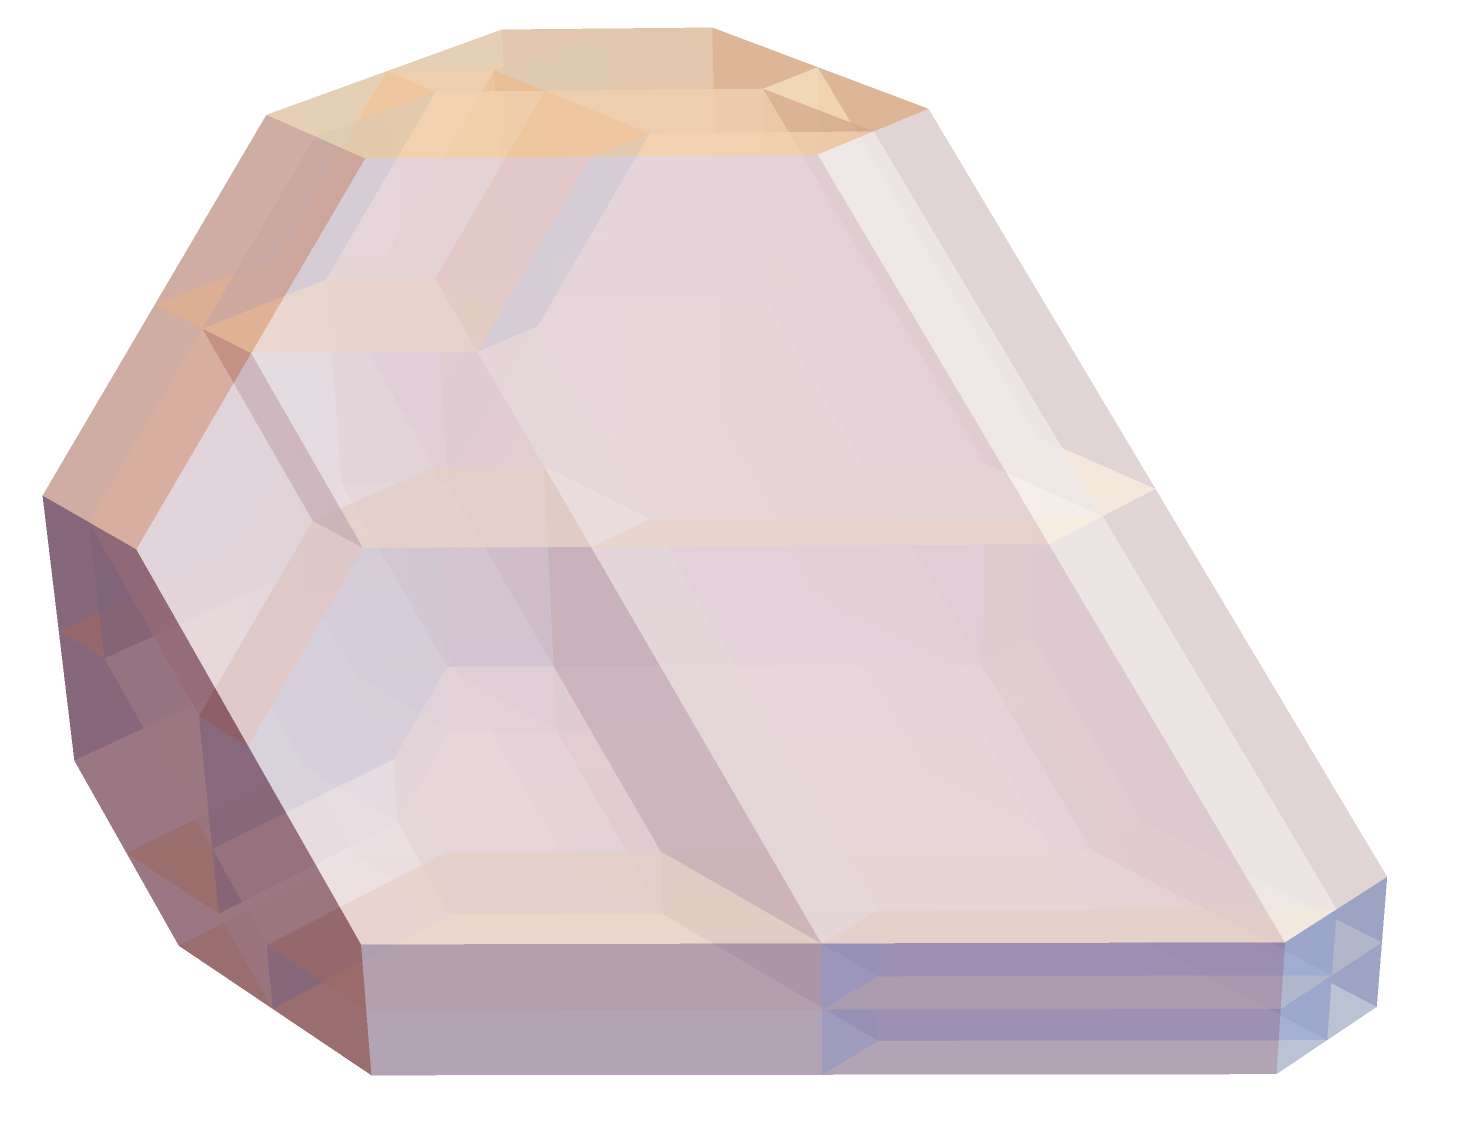
\includegraphics[width=0.7\linewidth]{J4.png} 
%\caption{The polytopal subdivision of $\J_4$.}
\label{Fig5:J4}
\end{figure}

\setcounter{tocdepth}{1}
\tableofcontents

%%%%%%%%%%%%%%%%%%%%%%%%%%%%%%%%%%%%%%%%

\section*{Introduction}

\rouge{Retaper l'introduction à la toute fin}

\rouge{Corriger leftmargin partout où nécessaire}

\rouge{Décider à la fin ce qu'on met en Théorème et en Proposition}

The $n$-dimensional associahedron, a polytope whose faces are in bijection with planar trees with $n+1$ leaves, was first introduced as a topological cell complex by J. Stasheff to describe algebras whose product is associative only up to homotopy \cite{Stasheff63}.
The problem of giving polytopal realizations of these CW-complexes has a rich history \cite{CeballosZiegler12}, and the algebras that they encode, called $\mathrm{A}_\infty$-algebras, are classical objects in algebraic topology. 
They have found many applications, from iterated loop spaces \cite{May72} to Fukaya categories \cite{Seidel08}, through the interpretation of the associahedra as moduli spaces of metric trees \cite{MauWoodward10}.
Today, this notion is ubiquitous and appears in different branches of mathematics such as symplectic topology, mathematical physics, mirror symmetry, Galois cohomology or non-commutative probability.

\medskip

The $n$-dimensional multiplihedron, a polytope whose faces are in bijection with 2-colored planar trees with $n$ leaves (see \cref{def:2coloredtree}), was first introduced as a topological cell complex by J. Stasheff to describe morphisms between $\mathrm{A}_\infty$-algebras \cite{Stasheff70}.
It was only realized as a convex polytope recently, through the work of S. Forcey \cite{Forcey08}, and later S. Forcey and S. Devadoss \cite{DevadossForcey08}, F. Ardila and J. Doker \cite{AD13}, and F. Chapoton and V. Pilaud \cite{CP22}.
The family of multiplihedra was studied both in algebraic topology \cite{BoardmanVogt73} and symplectic topology \cite{MauWoodward10,Mazuir21}, through their interpretation as moduli spaces of 2-colored metric trees. 

\medskip

In this paper, we define and study a cellular approximation to the diagonal of the multiplihedron. 
The need for such an approximation comes from the general fact that the set-theoretic diagonal $\triangle_P:P\to P\times P, x\mapsto (x,x)$ of a polytope $P$ is not cellular, that is, its image is not a union of faces of $P\times P$. 
A cellular approximation of the diagonal is a cellular map $\triangle_P^{\textrm{cell}} : P \to P\times P$ which is homotopic to $\triangle_P$ and which agrees with $\triangle_P$ on the vertices of $P$.

\medskip

The Alexander--Whitney map \cite{EilenbergMacLane53} and the Serre diagonal \cite{Serre51} are cellular approximations of the diagonal of the simplices and the cubes, respectively. 
They allow one to define the cup product in cohomology.
A cellular approximation of the diagonal of the associahedra allows one to define the tensor product of two $\mathrm{A}_\infty$-algebras \cite{SaneblidzeUmble04,MarklShnider06,MTTV19}. 
Our goal here is to make this tensor product COMPLETER

\medskip

Our results can be summarized as follows.
\begin{enumerate}[leftmargin=*]
  \item We define a cellular approximation of the diagonal of the Forcey--Loday realizations of the multiplihedra (\cref{prop:OrientationVector});
  \item We endow them with a compatible topological cellular operadic bimodule structure over the Loday realizations of the associahedra (\cref{thm:MainOperad});
  \item We describe combinatorially the cellular image of the diagonal (\cref{thm:formuladiagonal});
  \item We apply the cellular chains functor to define the tensor product of $\mathrm{A}_\infty$-algebras and their categorification, known as $\mathrm{A}_\infty$-categories (\cref{prop:tensorproduct}).
\end{enumerate}


To achieve these goals, we use the general theory developed by the first author in \cite{LA21}, based on the method introduced in \cite{MTTV19}.
For this purpose, we use the extra idea that the Forcey--Loday realization of the multiplihedron, as defined in \cite{Forcey08}, can be obtained from the Ardila--Doker realization of the multiplihedron \cite{AD13} by projection.
This last realization is a generalized permutahedron, in the sense of A. Postnikov \cite{Postnikov09}, which allows us to apply the results of \cite{LA21} directly, both for the purpose of defining a cellular approximation of the diagonal, and to describe its cellular image combinatorially.

\medskip

Our methods provide us with an universal tensor product, in the sense that its formula applies to any pair of $\Ainf$-morphisms.
Let us call such a tensor product \emph{operadic}. 
Unfortunately, our tensor product does not define a functor, since it is not strictly compatible with the composition of $\Ainf$-morphisms. 
This is not a defect of our construction: in \cref{thm:nofunctorial}, we prove that there is no operadic tensor product satisfying this property. 
The proof is similar to a result of M. Markl and S. Schnider saying that there is no operadic tensor product of $\Ainf$-algebras that satisfies associativity \cite[Theorem 13]{MarklShnider06}.
Our tensor product of $\Ainf$-morphisms could still be a functor in some homotopical sense, and we examine in \cref{sec:monoidality} different perspectives regarding the possibility of endowing the category of $\Ainf$-algebras with a (homotopy) symmetric monoidal structure. 

\medskip

Our results can readily be applied to different fields, prominently to symplectic topology. 
First, the operadic bimodule structure in~(2) above was used in the work of the second author, where the structures of $\mathrm{A}_\infty$-algebras and $\mathrm{A}_\infty$-morphisms are unraveled in the context of Morse theory \cite{Mazuir21}. 
Second, our definition of a tensor product of $\mathrm{A}_\infty$-categories by explicit formulae can be used to study the product of Fukaya algebras of Lagrangians \cite{amorim-lagrangian}, and more generally the product of Fukaya categories of symplectic manifolds. 
%deformations of bordered Riemann surfaces and the work of Liu
It could also be used in the context of bordered Heegaard Floer homology \cite{LOT20}. 
These applications are sketched in more details in \cref{sec:furtherdirections}.
One could also think to applications in other areas where the multiplihedron appears, such as higher category theory \cite{ForceyQuotient08}.

\medskip

Finally, the methods of this paper can be straightfowardly extended to the "multiploperahedra", a family of polytopes which is to the operahedra of \cite{LA21} what the multiplihedra are to the associahedra. 
They belong to both the families of graph-multiplihedra \cite{DevadossForcey08} and nestomultiplihedra \cite{AD13}.  
Together with the results of \cite{LA21}, one would obtain a tensor product of $\infty$-morphisms between homotopy operads, defined by explicit formulae. 

\subsection*{Layout} 
We define the realizations of the multiplihedra we will work with in \cref{sec:I}. 
We define a cellular approximation of their diagonal and endow them with an operadic bimodule structure over the associahedra in \cref{sec:II}.
We describe explicitly the image of our diagonal combinatorially, define the tensor product of $\mathrm{A}_\infty$-morphisms, and sketch applications to symplectic topology in \cref{sec:III}. 

\subsection*{Conventions} We use the conventions and notations of \cite{Ziegler95} for convex polytopes and the ones of \cite{LodayVallette12} for operads. We denote by $[n]\coloneqq \{1,\ldots,n\}$ and by $\{ e_i\}_{i \in [n]}$ the standard basis of $\RR^n$.

\subsection*{Acknowledgements} 
We would like to thank Bruno Vallette for numerous discussions and for his careful reading of the manuscript, and Eric Hoffbeck for his comments on an earlier version.
We are indebted to Lino Amorim and Robert Lipshitz, for explaining to us their work and for their detailed insights about possible applications of our results in symplectic topology.


%%%%%%%%%%%%%%%%%%%%%%%%%%%%%%%%%%%%%%%%%%%%

\section{Realizations of the multiplihedra} 
\label{sec:I}

Drawing from the work of S. Forcey in \cite{Forcey08}, we define weighted Forcey--Loday realizations of the multiplihedra and describe their general properties using the methods of \cite{MTTV19}.
We then show how they can be recovered from the Ardila--Doker realizations of the multiplihedra.

%%%%%%%%%%%%%%%%%%%%%%%%%%%%%%%%%%%%%%%%%%%%%

\subsection{2-colored trees and multiplihedra}

\subsubsection{2-colored trees}

We consider in this section \textit{planar rooted trees}, which we simply abbreviate as \textit{trees}. The term \emph{edge} refers to both internal and external edges. The external edges will sometimes be called leaves. 

\begin{definition}[Cut]
A \emph{cut} of a tree is a subset of edges or vertices which contains precisely one edge or vertex in each non-self crossing path from an incoming edge to the root.
\end{definition}

\noindent A cut divides a tree into an upper part that we color in blue and a lower part that we color in red. The edges and vertices of the cut are moreover represented by drawing a black line over them. See Figure \ref{Fig1:2ColTree} for an example. 

\begin{definition}[2-colored tree] \label{def:2coloredtree}
A \emph{2-colored tree} is a tree together with a cut. We call \emph{2-colored maximal tree} a 2-colored binary tree whose cut is made of edges only. 
\end{definition}
\noindent We denote by $\CT{n}$ (resp. $\CMT{n}$) the set of 2-colored trees (resp. 2-colored maximal trees) with $n$ leaves, for $n\geq 1$. 

\begin{figure}[h]
\[\vcenter{\hbox{
\begin{tikzpicture}[yscale=0.7,xscale=1]
%\draw[help lines] (-3,-1) grid (4,3);
%TOP
\draw[very thick, MidnightBlue] (-2.5,3.5)--(-2,2.5);
\draw[very thick, MidnightBlue] (-1.5,3.5)--(-2,2.5);
\draw[very thick, MidnightBlue] (-2,2.5) -- (-1.75,2);
\draw[very thick, MidnightBlue] (-1.25, 2) -- (-1,2.5);
\draw[very thick, MidnightBlue] (-0.5,2.5) -- (0,1.5);
\draw[very thick, MidnightBlue] (0,1.5)--(0,2.5);
\draw[very thick, MidnightBlue] (0,1.5)--(0.5,2.5);
\draw[very thick, MidnightBlue] (1,1)--(1.5,1.5);
\draw[very thick, MidnightBlue] (1.5,1.5)--(1,2.5);
\draw[very thick, MidnightBlue] (1.5,1.5)--(2,2.5);
\draw[very thick, MidnightBlue] (2,2.5)--(1.5,3.5);
\draw[very thick, MidnightBlue] (2,2.5)--(2,3.5);
\draw[very thick, MidnightBlue] (2,2.5)--(2.5,3.5);
%BOT
\draw[very thick, BrickRed] (0,-1)--(0, 1.5); 
\draw[very thick, BrickRed] (0,0)--(-1.5,1.5);
\draw[very thick, BrickRed] (-1.5,1.5)--(-1.75, 2); 
\draw[very thick, BrickRed] (-1.5,1.5)--(-1.25, 2); 
\draw[very thick, BrickRed] (0,0)--(1, 1);
% Frontier
\draw (-2,2) to (-1,2); 
\draw (-0.25,1.5)-- (0.25, 1.5) ; 
\draw (0.75,1) to (1.25,1);
\end{tikzpicture}}}\]
\caption{An example of a 2-colored tree.}
\label{Fig1:2ColTree}
\end{figure}

\begin{definition}[Face order]\leavevmode
The \emph{face order} $s\subset t$ on 2-colored trees is defined as follows: a 2-colored tree $s$ is less than a 2-colored tree $t$ if $t$ can be obtained from $s$ by a sequence of contractions of monochrome edges or moves of the cut from an edge to an adjacent vertex.

\begin{figure}[h]
\[\vcenter{\hbox{
\begin{tikzpicture}[yscale=0.7,xscale=1]
%TOP
\draw[very thick, MidnightBlue] (-2.5,3.5)--(-2,2.5);
\draw[very thick, MidnightBlue] (-1.5,3.5)--(-2,2.5);
\draw[very thick, MidnightBlue] (-2,2.5) -- (-1.75,2);
\draw[very thick, MidnightBlue] (-1.25, 2) -- (-1,2.5);
\draw[very thick, MidnightBlue] (-0.5,2.5) -- (0,1.5);
\draw[very thick, MidnightBlue] (0,1.5)--(0,2.5);
\draw[very thick, MidnightBlue] (0,1.5)--(0.5,2.5);
\draw[very thick, MidnightBlue] (1,1)--(1.5,1.5);
\draw[very thick, MidnightBlue] (1.5,1.5)--(1,2.5);
\draw[very thick, MidnightBlue] (1.5,1.5)--(2,2.5);
\draw[very thick, MidnightBlue] (2,2.5)--(1.5,3.5);
\draw[very thick, MidnightBlue] (2,2.5)--(2,3.5);
\draw[very thick, MidnightBlue] (2,2.5)--(2.5,3.5);
%BOT
\draw[very thick, BrickRed] (0,-1)--(0, 1.5); 
\draw[very thick, BrickRed] (0,0)--(-1.5,1.5);
\draw[very thick, BrickRed] (-1.5,1.5)--(-1.75, 2); 
\draw[very thick, BrickRed] (-1.5,1.5)--(-1.25, 2); 
\draw[very thick, BrickRed] (0,0)--(1, 1);
% Frontier
\draw (-2,2) to (-1,2); 
\draw (-0.25,1.5)-- (0.25, 1.5) ; 
\draw (0.75,1) to (1.25,1);
\end{tikzpicture}}}
\quad \subset \quad
\vcenter{\hbox{
\begin{tikzpicture}[yscale=0.7,xscale=1]
%TOP
\draw[very thick, MidnightBlue] (-1.5,1.5)--(-1.5,2.5);
\draw[very thick, MidnightBlue] (-2,2.5) -- (-1.75,2);
\draw[very thick, MidnightBlue] (-1.25, 2) -- (-1,2.5);
\draw[very thick, MidnightBlue] (-0.5,2.5) -- (0,1.5);
\draw[very thick, MidnightBlue] (0,1.5)--(0,2.5);
\draw[very thick, MidnightBlue] (0,1.5)--(0.5,2.5);
\draw[very thick, MidnightBlue] (1,1)--(1.5,1.5);
\draw[very thick, MidnightBlue] (1.5,1.5)--(1,2.5);
\draw[very thick, MidnightBlue] (1.5,1.5)--(1.33,2.5);
\draw[very thick, MidnightBlue] (1.5,1.5)--(1.66,2.5);
\draw[very thick, MidnightBlue] (1.5,1.5)--(2,2.5);
\draw[very thick, MidnightBlue] (-1.5,1.5)--(-1.75, 2); 
\draw[very thick, MidnightBlue] (-1.5,1.5)--(-1.25, 2); 
%BOT
\draw[very thick, BrickRed] (0,-1)--(0, 1.5); 
\draw[very thick, BrickRed] (0,0)--(-1.5,1.5);
\draw[very thick, BrickRed] (0,0)--(1, 1);
% Frontier
\draw (-1.75,1.5) to (-1.25,1.5); 
\draw (-0.25,1.5) to (0.25,1.5); 
\draw (0.75,1) to (1.25,1);
\end{tikzpicture}}}
\]
\caption{An example of the face order $s\subset t$.}
\label{Fig2:InclusionOrder}
\end{figure}

\end{definition}


\begin{definition}[Tamari-type order]\leavevmode
The \emph{Tamari-type order} $s<t$ on  2-colored maximal trees is generated by the following three  covering relations: 
\[
{\vcenter{\hbox{
\begin{tikzpicture}[yscale=0.5,xscale=0.5]
\draw[very thick, MidnightBlue] (0,-0.5)--(0,0) -- (-2,2)--(-2,2.5);
\draw[very thick, MidnightBlue] (-1,1)--(0,2)--(0,2.5) ;
\draw[very thick, MidnightBlue] (0,0)--(1,1)--(1,2.5) ;
%
\draw[very thick, BrickRed] (0,-0.5)--(0,-1) ;
%
\draw (-0.5,-0.5) --(0.5, -0.5);
%
\draw (-2,2.5) node[above] {$t_1$}; 
\draw (0,2.5) node[above] {$t_2$}; 
\draw (1,2.5) node[above] {$t_3$}; 
\draw (0,-1) node[below] {$t_4$}; 
\end{tikzpicture}}}}
\prec
{\vcenter{\hbox{
\begin{tikzpicture}[yscale=0.5,xscale=0.5]
\draw[very thick, MidnightBlue] (0,-0.5)--(0,0) -- (2,2)--(2,2.5);
\draw[very thick, MidnightBlue] (1,1)--(0,2)--(0,2.5) ;
\draw[very thick, MidnightBlue] (0,0)--(-1,1)--(-1,2.5) ;
%
\draw[very thick, BrickRed] (0,-0.5)--(0,-1) ;
%
\draw (-0.5,-0.5) --(0.5, -0.5);
%
\draw (2,2.5) node[above] {$t_3$}; 
\draw (0,2.5) node[above] {$t_2$}; 
\draw (-1,2.5) node[above] {$t_1$}; 
\draw (0,-1) node[below] {$t_4$}; 
\end{tikzpicture}}}}\ , \quad 
{\vcenter{\hbox{
\begin{tikzpicture}[yscale=0.5,xscale=0.5]
\draw[very thick, MidnightBlue] (-2, 2.5)--(-2, 3) ;
\draw[very thick, MidnightBlue] (0, 2.5)--(0, 3) ;
\draw[very thick, MidnightBlue] (1, 2.5)--(1, 3) ;
%
\draw[very thick, BrickRed] (0,-0.5)--(0,0) -- (-2,2)--(-2,2.5);
\draw[very thick, BrickRed] (-1,1)--(0,2)--(0,2.5) ;
\draw[very thick, BrickRed] (0,0)--(1,1)--(1,2.5) ;
%
\draw (-2.5,2.5) --(1.5, 2.5);
%
\draw (-2,3) node[above] {$t_1$}; 
\draw (0,3) node[above] {$t_2$}; 
\draw (1,3) node[above] {$t_3$}; 
\draw (0,-0.5) node[below] {$t_4$}; 
\end{tikzpicture}}}}
\prec
{\vcenter{\hbox{
\begin{tikzpicture}[yscale=0.5,xscale=0.5]
\draw[very thick, BrickRed] (0,-0.5)--(0,0) -- (2,2)--(2,2.5);
\draw[very thick, BrickRed] (1,1)--(0,2)--(0,2.5) ;
\draw[very thick, BrickRed] (0,0)--(-1,1)--(-1,2.5) ;
%
\draw[very thick, MidnightBlue] (2,2.5)--(2,3) ;
\draw[very thick, MidnightBlue] (0,2.5)--(0,3) ;
\draw[very thick, MidnightBlue] (-1,2.5)--(-1,3) ;
%
\draw (-1.5,2.5) --(2.5, 2.5);
%
\draw (2,3) node[above] {$t_3$}; 
\draw (0,3) node[above] {$t_2$}; 
\draw (-1,3) node[above] {$t_1$}; 
\draw (0,-0.5) node[below] {$t_4$}; 
\end{tikzpicture}}}}\ , \quad 
{\vcenter{\hbox{
\begin{tikzpicture}[yscale=0.5,xscale=0.5]
\draw[very thick, MidnightBlue] (0,0.5)--(0,1);
\draw[very thick, MidnightBlue] (0,1)--(-0.5,1.5)--(-0.5,2);
\draw[very thick, MidnightBlue] (0,1)--(0.5,1.5)--(0.5,2);
% 
\draw[very thick, BrickRed] (0,0)--(0,0.5);
\draw (-0.5,0.5) --(0.5, 0.5);
%
\draw (-0.5,2) node[above] {$t_1$}; 
\draw (0.5,2) node[above] {$t_2$}; 
\draw (0,0) node[below] {$t_3$}; 
\end{tikzpicture}}}}
\prec
{\vcenter{\hbox{
\begin{tikzpicture}[yscale=0.5,xscale=0.5]
\draw[very thick, MidnightBlue] (-0.5,2)--(-0.5,2.5);
\draw[very thick, MidnightBlue] (0.5,2)--(0.5,2.5);
%
\draw[very thick, BrickRed] (0,0.5)--(0,1);
\draw[very thick, BrickRed] (0,1)--(-0.5,1.5)--(-0.5,2);
\draw[very thick, BrickRed] (0,1)--(0.5,1.5)--(0.5,2);
% 
\draw (-1,2) --(1, 2);
%
\draw (-0.5,2.5) node[above] {$t_1$}; 
\draw (0.5,2.5) node[above] {$t_2$}; 
\draw (0,0.5) node[below] {$t_3$}; 
\end{tikzpicture}}}}
\ ,\]
where $t_i$, for $1\leq i\leq 4$, are 2-colored maximal trees, of respective colors each time. 
\end{definition}

\begin{figure}[h]
\[\vcenter{\hbox{
\begin{tikzcd}[column sep=0.5cm, row sep=0.5cm]
& \TreeLa \arrow[ld, thin] \arrow[rr, thin]&& \TreeRa \arrow[rd, thin]& \\
\TreeLb \arrow[rd, thin] &&&& \TreeRb \arrow[ld, thin] \\
& \TreeLc \arrow[rr, thin] && \TreeRc &
\end{tikzcd}
}}\]
\caption{The Tamari-type poset $(\CMT{3}, <)$ with minimum at the top.}
\label{Fig3:Tam}
\end{figure}

\noindent We add a minimum element $\emptyset_n$ to the poset of 2-colored trees $(\CT{n}, \subset)$. 

\begin{proposition}
The posets $(\CT{n}, \subset)$ and $(\CMT{n}, <)$ are lattices. 
\end{proposition}

\begin{proof}
The poset of 2-colored trees was proven in \cite{Forcey08} to be isomorphic to the face lattice of a polytope, the multiplihedron; see Point~(3) of \cref{prop:PropertiesKLoday}. 
The Hasse diagram of the poset of 2-colored maximal trees was proven to be isomorphic to the oriented 1-skeleton of the multiplihedron, and also to be the Hasse diagram of a lattice in \cite[Proposition 117]{CP22}.
\end{proof}

\begin{remark}
F. Chapoton and V. Pilaud introduce in \cite{CP22} the shuffle of two generalized permutahedra (see \cref{sec:generalizedpermutahedra} for definition and examples).
The fact that the poset $(\CMT{n}, <)$ is a lattice follows from the fact that the multiplihedron arises as the shuffle of the associahedron and the interval, which both have the lattice property, and that the shuffle operation preserves the lattice property in this case \cite[Corollary 95]{CP22}. 
\end{remark}

\subsubsection{Grafting of trees} \label{sss:grafting}

We will denote the operation of grafting a planar tree $v$ at the $i^{\rm th}$-leaf of a 2-colored tree $u$ by $u \circ_i v$. 
We will also denote the grafting of a level of 2-colored trees $v_1, \ldots, v_k$ on the $k$ leaves of a planar tree by $u(v_1, \ldots, v_k)$. 
We denote by $c^{\T}_n$ and by $c^{\B}_n$ the corollae with $n$ leaves fully painted with the upper and the lower color respectively; we denote by $c_n$ the corolla with $n$ leaves with frontier color at the vertex. 
It is straightforward to see that these two grafting operations on corollae generate all the 2-colored trees of codimension $1$: we call $(\B)$, for ``bottom'', the first type of 2-colored trees $c_{p+1+r}\circ_{p+1} c^\T_q$, with $p+q+r=n$ and $2\leq q\leq n$, and we call  $(\T)$, for ``top'', the second type of 2-colored trees $c^\B_k(c_1, \ldots, c_k)$, with $i_1+\cdots+i_k=n$, $i_1, \ldots,i_k\geq 1$, and $k\geq 2$.

\begin{figure}[h]
\[\vcenter{\hbox{
\begin{tikzpicture}[yscale=0.7,xscale=1]
%TOP
\draw[very thick, MidnightBlue] (0.5,1)--(0,2);
\draw[very thick, MidnightBlue] (0.5,1)--(0.5,2);
\draw[very thick, MidnightBlue] (0.5,1)--(1,2);
\draw[very thick, MidnightBlue] (0,0)--(0.5, 1); 
\draw[very thick, MidnightBlue] (0,0)--(-0.5, 1); 
\draw[very thick, MidnightBlue] (0,0)--(-1.5,1);
\draw[very thick, MidnightBlue] (0,0)--(1.5, 1);
%BOT
\draw[very thick, BrickRed] (0,-1)--(0, 0); 
% Frontier
\draw (-0.25,0) to (0.25,0); 
\draw (0,-2) node {type $(\B)$};
\end{tikzpicture}}}\qquad \vcenter{\hbox{
\begin{tikzpicture}[yscale=0.7,xscale=1]
%TOP
\draw[very thick, MidnightBlue] (-1.5,1)--(-1.5,2);
\draw[very thick, MidnightBlue] (-2,2) -- (-1.75,1.5);
\draw[very thick, MidnightBlue] (-1.25, 1.5) -- (-1,2);
\draw[very thick, MidnightBlue] (-0.5,2) -- (0,1);
\draw[very thick, MidnightBlue] (0,1)--(0.5,2);
\draw[very thick, MidnightBlue] (1.5,1)--(1,2);
\draw[very thick, MidnightBlue] (1.5,1)--(1.33,2);
\draw[very thick, MidnightBlue] (1.5,1)--(1.66,2);
\draw[very thick, MidnightBlue] (1.5,1)--(2,2);
\draw[very thick, MidnightBlue] (-1.5,1)--(-1.75, 1.5); 
\draw[very thick, MidnightBlue] (-1.5,1)--(-1.25, 1.5); 
%BOT
\draw[very thick, BrickRed] (0,-1)--(0, 1); 
\draw[very thick, BrickRed] (0,0)--(-1.5,1);
\draw[very thick, BrickRed] (0,0)--(1.5, 1);
% Frontier
\draw (-1.75,1) to (-1.25,1); 
\draw (-0.25,1) to (0.25,1); 
\draw (1.25,1) to (1.75,1);
\draw (0,-2) node {type $(\T)$};
\end{tikzpicture}}}\]
\caption{Examples of 2-colored trees of type $(\B)$ and $(\T)$ respectively. }
\label{Fig5:FacetsColoredTrees}
\end{figure}

%%%%%%%%%%%%%%%%%%%%%%%%%%%%%%%%%%%%%%%%%%%%%

\subsubsection{Multiplihedra} \label{sec:multiplihedra}

\begin{definition}[Multiplihedra]
For any $n\geq 1$, an \emph{$(n-1)$-dimensional multiplihedron} is a polytope of dimension $(n-1)$ whose face lattice is isomorphic to the lattice 
$(\CT{n}, \subset)$
of 2-colored trees with $n$ leaves. 
\end{definition}

\begin{figure}[h]
\[
\begin{tikzpicture}[xscale=0.8,yscale=1]
\draw[thick] (-2,2)--(2,2)--(4,0)--(2,-2)--(-2,-2)--(-4,0)--cycle;
\draw[fill, opacity=0.12] (-2,2)--(2,2)--(4,0)--(2,-2)--(-2,-2)--(-4,0)--cycle;
\draw (-2,2) node[above left] {$\TreeLa$};
\draw (2,2) node[above right] {$\TreeRa$};
\draw (-2,-2) node[below left] {$\TreeLc$};
\draw (2,-2) node[below right] {$\TreeRc$};
\draw (-4.2,0) node[left] {$\TreeLb$};
\draw (4,0) node[right] {$\TreeRb$};
\draw (-3,1) node[above left] {$\TreeLab$};
\draw (-3,-1) node[below left] {$\TreeLbc$};
\draw (3,1) node[above right] {$\TreeRab$};
\draw (3,-1) node[below right] {$\TreeRbc$};
\draw (0,2.1) node[above] {$\TreeCa$};
\draw (0,-2.1) node[below] {$\TreeCb$};
\draw (0,0) node  {$\TreeCab$};
\end{tikzpicture}
\]
\caption{A 2-dimensional multiplihedron.}
\label{Fig4:J3}
\end{figure}

The dimension of a face labeled by a 2-colored tree is given by the sum of the degrees of its vertices defined by 
\[
\left|{\vcenter{\hbox{
\begin{tikzpicture}[scale=0.5]
\draw[very thick, MidnightBlue] (0,-0.5) -- (0,1.5);
\draw[very thick, MidnightBlue] (0,0) -- (-1,1)--(-1,1.5);
\draw[very thick, MidnightBlue] (0,0) -- (1,1)--(1,1.5);
\draw (1,1.5) node[above] {$k$};
\draw (-1,1.5) node[above] {$1$};
\draw (0,1.5) node[above] {$\cdots$};
\end{tikzpicture}}}}\right|=k-2\ , \quad 
\left|{\vcenter{\hbox{
\begin{tikzpicture}[scale=0.5]
\draw[very thick, BrickRed] (0,-0.5) -- (0,1.5);
\draw[very thick, BrickRed] (0,0) -- (-1,1)--(-1,1.5);
\draw[very thick, BrickRed] (0,0) -- (1,1)--(1,1.5);
\draw (1,1.5) node[above] {$k$};
\draw (-1,1.5) node[above] {$1$};
\draw (0,1.5) node[above] {$\cdots$};
\end{tikzpicture}}}}\right|=k-2\ , \quad 
\left|{\vcenter{\hbox{
\begin{tikzpicture}[scale=0.5]
\draw[very thick, MidnightBlue] (0,0) -- (0,1.5);
\draw[very thick, MidnightBlue] (0,0) -- (-1,1)--(-1,1.5);
\draw[very thick, MidnightBlue] (0,0) -- (1,1)--(1,1.5);
\draw[very thick, BrickRed] (0,0) -- (0,-0.5);
\draw (-0.5,0)--(0.5,0);
\draw (1,1.5) node[above] {$k$};
\draw (-1,1.5) node[above] {$1$};
\draw (0,1.5) node[above] {$\cdots$};
\end{tikzpicture}}}}\right|=k-1\ .
\]
The codimension of a 2-colored tree is then in particular equal to the number of blue vertices and red vertices. 
In the example of the 2-colored tree depicted on \cref{Fig1:2ColTree}, the dimension is equal to 4 and the codimension is equal to 5. 
As proven in \cite[Proposition 117]{CP22}, the oriented $1$-skeleton of a multiplihedron is the Hasse diagram of the Tamari-type poset. 

%%%%%%%%%%%%%%%%%%%%%%%%%%%%%%%%%%%%%%%%%%%%

\subsection{Forcey--Loday realizations of the multiplihedra}
Jean-Louis Loday gave in \cite{Loday04a} realizations of the associahedra in the form of polytopes with integer coordinates. 
Stefan Forcey generalized this construction in \cite{Forcey08} in order to give similar realizations for the multiplihedra. 
In this subsection we adapt the ideas of \cite{MTTV19} to the multiplihedra of Forcey and define realizations of the multiplihedra associated to any weight $\omega$. We refer to them as \emph{Forcey--Loday realizations} of the multiplihedra.

\begin{definition}[Weighted 2-colored maximal tree]
A \emph{weighted 2-colored maximal tree} is a pair $(t, \omega)$ made up of a 2-colored maximal tree $t\in \CMT{n}$ with $n$ leaves with a weight $\omega= (\omega_1, \ldots, \omega_n) \in \RR_{>0}^n$. 
We call $\omega$ the \emph{weight} and $n$ the \emph{length} of the weight $\omega$.
\end{definition}

Let $(t, \omega)$ be a weighted 2-colored maximal tree with $n$ leaves. We order its $n-1$ vertices from left to right. At the $i^{\rm th}$ vertex, we consider the sum $\alpha_i$ of the weights of the leaves supported by its left input and 
 the sum $\beta_i$ of the weights of the leaves supported by its right input. 
If the $i^{\rm th}$ vertex is colored by the upper color, we consider the product $\alpha_i\beta_i$ and if the 
$i^{\rm th}$ vertex is colored by the lower color, we consider the product $2\alpha_i\beta_i$.
The associated string produces a point with integer coordinates :
\[M(t, \omega) \coloneqq \big(2\alpha_1\beta_1, \alpha_2\beta_2, \ldots, 2\alpha_{n-1}\beta_{n-1}\big)\in 
\RR_{>0}^{n-1}\ . \]
\begin{figure}[h!]
\[
\vcenter{\hbox{\begin{tikzpicture}[scale=1.5]
\draw[thick] (1,0)--(2,0);
\draw (1,0) node[above] {$\TreeBa$};
\draw (1.95,0) node[above] {$\TreeBb$};
\draw (1,0) node[below] {$1$};
\draw (2,0) node[below] {$2$};
\end{tikzpicture}}} \qquad \qquad
\vcenter{\hbox{
\begin{tikzpicture}[scale=1.5]
\draw (1,-0.05)--(1,0.05);
\draw (2,-0.05)--(2,0.05);
\draw (3,-0.05)--(3,0.05);
\draw (4,-0.05)--(4,0.05);
\draw (-0.05, 1)--(0.05,1);
\draw (-0.05, 2)--(0.05,2);
\draw (-0.05, 3)--(0.05,3);
\draw (-0.05, 4)--(0.05,4);
\draw[->] (0,0)--(5,0);
\draw[->] (0,0)--(0,5);
\draw (1,0) node[below] {$1$};
\draw (2,0) node[below] {$2$};
\draw (3,0) node[below] {$3$};
\draw (4,0) node[below] {$4$};
\draw (0,1) node[left] {$1$};
\draw (0,2) node[left] {$2$};
\draw (0,3) node[left] {$3$};
\draw (0,4) node[left] {$4$};
\draw[thick] (1,2)--(1,4)--(2,4)--(4,2)--(4,1)--(2,1)--cycle;
\draw (1,2) node[below left] {$\TreeLa$};
\draw (2,1) node[below left] {$\TreeRa$};
\draw (2,4) node[above right] {$\TreeLc$};
\draw (4,2) node[above right] {$\TreeRc$};
\draw (1,4) node[above left] {$\TreeLb$};
\draw (4,1) node[below right] {$\TreeRb$};
\end{tikzpicture}}}
\]
\caption{Examples of points associated to 2-colored maximal trees, with trivial weight.}
\end{figure}


\begin{definition}[Forcey--Loday Realization] \label{def:ForceyLoday}
 The \emph{Forcey--Loday realization of weight $\omega$} of the $(n-1)$-dimensional multiplihedron is the  polytope
\[\J_\omega \coloneqq \conv \big\{M(t, \omega)\mid t\in \CMT{n} \big\}\subset \RR^{n-1}\ .\]
\end{definition}

The Forcey--Loday realization associated to the standard weight $(1, \ldots, 1)$ will simply be denoted by $\J_n$.
By convention, we define the polytope $\J_\omega$ with weight $\omega=(\omega_1)$ of length $1$  to be made up of one point labeled by the 2-colored  tree $\iBT\coloneq \TreeIab$\ .
\begin{figure}[h]
\[
\begin{tikzpicture}[scale=0.8, J4]
\draw[->] (4,-4,-3)--(5,-4,-3) node[below left] {$x_1$};
\draw[->] (4,-4,-3)--(4,-3, -3) node[below right] {$x_2$};
\draw[->] (4,-4,-3)--(4,-4,-2) node[above] {$x_3$};

\draw[thick, opacity=0.2] (1,4,1)--(1,2,3)--(2,1,3)--(3,1,2)--(3,2,1)--cycle;
\draw[thick] (2,8,2)--(2,4,6)--(4,2,6)--(6,2,4)--(6,4,2)--cycle;
\draw[thick] (4,1,6)--(6,1,4)--(6,1,2)--(6,2,1)--(6,4,1)--(2,8,1)--(1,8,1)--(1,8,2)--(1,4,6)--(1,2,6)--(2,1,6)--cycle;
\draw[thick] (4,1,6)--(4,2,6);
\draw[thick] (6,1,4)--(6,2,4);
\draw[thick, opacity=0.2] (6,1,2)--(3,1,2);
\draw[thick, opacity=0.2] (6,2,1)--(3,2,1);
\draw[thick] (6,4,1)--(6,4,2);
\draw[thick] (2,8,1)--(2,8,2)--(1,8,2);
\draw[thick, opacity=0.2] (1,8,1)--(1,4,1);
\draw[thick] (1,4,6)--(2,4,6);
\draw[thick, opacity=0.2] (1,2,6)--(1,2,3);
\draw[thick, opacity=0.2] (2,1,6)--(2,1,3);

\draw[fill, opacity=0.12] (2,8,2)--(2,4,6)--(4,2,6)--(6,2,4)--(6,4,2)--cycle;
\draw[fill, opacity=0.18] (6,2,4)--(6,1,4)--(6,1,2)--(6,2,1)--(6,4,1)--(6,4,2)--cycle;
\draw[fill, opacity=0.18] (6,2,4)--(6,1,4)--(4,1,6)--(4,2,6)--cycle;
\draw[fill, opacity=0.18] (4,1,6)--(4,2,6)--(2,4,6)--(1,4,6)--(1,2,6)--(2,1,6)--cycle;
\draw[fill, opacity=0.06] (2,8,2)--(6,4,2)--(6,4,1)--(2,8,1)--cycle;
\draw[fill, opacity=0.06] (2,8,1)--(2,8,2)--(1,8,2)--(1,8,1)--cycle;
\draw[fill, opacity=0.06] (2,8,2)--(1,8,2)--(1,4,6)--(2,4,6)--cycle;
\end{tikzpicture}
\]
\caption{The Forcey--Loday realization of the multiplihedron $\J_4$%, see \cref{prop:OrientationVector} for the definition of the $\vec e_i$.}
}
\end{figure}


\begin{proposition}\label{prop:PropertiesKLoday}
The Forcey--Loday realization $\J_\omega$  satisfies the following properties. 
\begin{enumerate}[leftmargin=*]
\item Let $t\in \CMT{n}$ be a 2-colored maximal tree. 

\noindent For $p+q+r=n$, with $2\leq q\leq n$, the point $M(t, \omega)$ is contained in the half-space defined by the inequality
\begin{equation}\label{Eq:B}\tag{$\B$}
x_{p+1}+\cdots+x_{p+q-1}\geq \sum_{p+1\leq a<b\leq p+q} \omega_a \omega_b\ , 
\end{equation}
with equality if and only if the 2-colored maximal tree $t$ can be decomposed as $t=u\circ_{p+1} v$, where $u\in\CMT{p+1+r}$ and $v\in \Tam{q}$. 

\noindent For $i_1+\cdots+i_k=n$, with $i_1, \ldots,i_k\geq 1$ and $k\geq 2$, the point $M(t, \omega)$ is contained in the half-space defined by the inequality
\begin{equation}\label{Eq:T}\tag{$\T$}
x_{i_1}+x_{i_1+i_2}+\cdots+x_{i_1+\cdots+i_{k-1}}\leq 
2\sum_{1\leq j<l\leq k} \omega_{I_j} \omega_{I_l}\ , 
\end{equation}
where $I_j=[i_1+\cdots +i_{j-1}+1, \ldots, i_1+\cdots +i_j]$ and $\omega_{I_j}\coloneq\sum_{a\in I_j} \omega_a$, with equality if and only if the 2-colored maximal tree $t$ can be decomposed as $t=u(v_1, \ldots, v_k)$, where $u\in\Tam{k}$ and $v_j\in \CMT{i_j}$, for $1\leq j\leq k$. 


\item The polytope $\J_\omega$ is the intersection of the half-spaces defined in  \emph{(1)}. 

\item The face lattice $(\La(\J_\omega), \subset)$ is isomorphic to the lattice $(\CT{n}, \subset)$ of 2-colored trees with $n$ leaves.

\item Any face of a Forcey--Loday realization of a multiplihedron is isomorphic to a product of a Loday realization of an associahedron with possibly many Forcey--Loday realizations of multiplihedra, via a permutation of coordinates. 
\end{enumerate}
\end{proposition}

\begin{proof}

Points~(1)--(3) were proved in \cite{Forcey08}.  
We prove Point~(4) by induction on $n$. 
It clearly holds true for $n=1$. Let us suppose that it holds true up to $n-1$ and let us prove it for the polytopes $\J_\omega$, for any weight $\omega$ of length $n$.
We examine first facets. 
In the case of a facet of type $(\B)$ associated to $p+q+r=n$ with $2\leq q \leq n-1$, we consider the following two weights 
\[
\overline{\omega}\coloneqq (\omega_1, \ldots, \omega_{p}, \omega_{p+1}+\cdots+\omega_{p+q}, \omega_{p+q+1}, \ldots,  \omega_{n})
\quad \text{and} \quad 
\widetilde{\omega}\coloneqq (\omega_{p+1}, \ldots, \omega_{p+q})
\]
and the isomorphism 
\begin{align*}
\begin{array}{rccc}
\Theta_{p,q,r}\  : &  \RR^{p+r}\times \RR^{q-1} &\xrightarrow{\cong} &\RR^{n-1}\\
&(x_1, \ldots, x_{p+r})\times (y_1, \ldots, y_{q-1}) & \mapsto& 
(x_1, \ldots, x_{p} , y_1, \ldots, y_{q-1}, x_{p+1}, \ldots, x_{p+r})\ .
\end{array}
\end{align*}
The image of the vertices of $\J_{\overline{\omega}}\times \K_{\widetilde{\omega}}$ are sent to the vertices of the facet of $\J_\omega$
labelled by the 2-colored tree $c_{p+1+r}\circ_{p+1} c^\T_q$. 
In other words, the permutation of coordinates $\Theta$ sends bijectively $\J_{\overline{\omega}}\times \K_{\widetilde{\omega}}$ to $\J_\omega$. 
Similarly, in the case of a facet of type $(\T)$ associated to $i_1+\cdots+i_k=n$ with 
$i_1, \ldots,i_k\geq 1$ and $k\geq 2$, 
 we consider the following weights 
%
\[
\overline{\omega}\coloneqq \big(\sqrt{2}\omega_{I_1}, \ldots, \sqrt{2}\omega_{I_k}\big)
\quad \text{and} \quad 
\widetilde{\omega}_j\coloneqq (\omega_{i_1+\cdots+i_{j-1}+1}, \ldots, \omega_{i_1+\cdots+i_{j-1}+i_j}), \ \text{for}\ 1\leq j\leq k, 
\]
and the isomorphism 
\begin{align*}
\begin{array}{rccc}
\Theta^{i_1, \ldots, i_k}\  : &  \RR^{k-1}\times \RR^{i_1-1}\times \cdots \times \RR^{i_k-1} &\xrightarrow{\cong} &\RR^{n-1}
\end{array}
\end{align*}
which sends 
\[(x_1, \ldots, x_{k-1})\times (y_1^1, \ldots, y^1_{i_1-1})\times \cdots 
\times (y_1^k, \ldots, y^k_{i_k-1})\]
to 
\[(
y^1_1,\ldots, y^1_{i_1-1}, x_1, y^2_1, \ldots, y^2_{i_2-1}, x_2, y^3_1, \ldots, x_{k-1}, y^k_1, \ldots, y^k_{i_k-1}
)\ .\]
The image of the vertices of 
$\K_{\overline{\omega}}\times \J_{\widetilde{\omega}_1}\times \cdots \times \J_{\widetilde{\omega}_k}$ are sent to the vertices of the facet of $\J_\omega$
labelled by the 2-colored tree $c^\B_k(c_1, \ldots, c_k)$. In other words, the permutation of coordinates $\Theta$ sends bijectively $\K_{\overline{\omega}}\times \J_{\widetilde{\omega}_1}\times \cdots \times \J_{\widetilde{\omega}_k}$ to $\J_\omega$. 

We can finally conclude the proof with these decompositions of facets of $\J_\omega$, the induction hypothesis, and \cite[Proposition~1, Point~(5)]{MTTV19}.
\end{proof}

%%%%%%%%%%%%%%%%%%%%%%%%%%%%%%%%%%%%

\subsection{Ardila-Doker realizations of the multiplihedra} 
\label{sec:generalizedpermutahedra}

\begin{definition}[Permutahedron] The \emph{$(n-1)$-dimensional permutahedron} is the polytope in $\RR^n$ equivalently defined as:
\begin{itemize}[leftmargin=*]
  \item the convex hull of the points $\displaystyle \sum_{i=1}^{n}i\vec e_{\sigma(i)}$ for all permutations $\sigma \in \mathbb{S}_n$, or
  \item the intersection of the hyperplane $\displaystyle  \left\{x \in \RR^n \ \bigg| \ \sum_{i=1}^{n} x_i = \binom{n+1}{2}\right\}$ with the affine half-spaces $\displaystyle \left\{x \in \RR^n \ \bigg| \ \sum_{i \in I} x_i \geq \binom{|I|+1}{2}\right\}$ for all $\emptyset\neq I \subseteq [n]$.
\end{itemize}
\end{definition}

\rouge{Rappeler ici les définitions de cône normal et éventail normal}

\begin{definition}[Generalized permutahedron]
A \emph{generalized permutahedron} is a polytope equivalently defined as:
\begin{itemize}[leftmargin=*]
\item a polytope whose normal fan coarsens the one of the permutahedron, or 
\item the convex set \[ \left\{ x \in \RR^n \ : \ \sum_{i=1}^{n}x_i = z_{[n]} \ , \sum_{i \in I} x_i \geq z_I \text{ for all } I \subseteq [n] \right\} \ , \]
where $\{ z_I \}_{I \subseteq [n]}$ are real numbers which satisfy the inequalities $z_I+z_J \leq z_{I\cup J} + z_{I \cap J}$ for all $I,J \subseteq [n]$, and where $z_\emptyset =0$.
\end{itemize}
\end{definition}

Generalized permutahedra were introduced by A. Postnikov \cite{Postnikov09}, and are subject of a vast literature. 
They present many interesting combinatorial, geometric and algebraic properties. 
For instance, they are the universal family of polytopes possessing a certain Hopf algebraic structure \cite{AguiarArdila17}. \rouge{soit étoffer ce paragraphe, soit le supprimer}

Loday realizations of the associahedra are all generalized permutahedra as proven in \cite{}, while Forcey--Loday realizations of the multiplihedra are not. 
However, F. Ardila and J. Doker introduced in \cite{AD13} realizations of the multiplihedra that are generalized permutahedra. 
They are obtained from the Loday realizations of the associahedra via the operation of \emph{$q$-lifting}. 
We will consider the special case $q=1/2$ of their construction.

\begin{definition}[Lifting of a generalized permutahedron {\cite[Definition 2.3]{AD13}}]
For a generalized permutahedron $P\subset \RR^n$, its \emph{$\tfrac{1}{2}$-lifting} $P \left(\tfrac{1}{2}\right) \subset \RR^{n+1}$ is defined by 
\[P \left(\tfrac{1}{2}\right) \coloneqq \left\{ x \in \RR^{n+1} \ : \ 
\sum_{i=1}^{n+1} x_i = z_{[n]} \ , 
\sum_{i \in I} x_i \geq \tfrac{1}{2}z_I \ ,
\sum_{i \in I \cup \{n+1\}} x_i \geq z_I 
\text{ for all } I \subseteq [n] \right\} \ . \]
\end{definition}

\begin{proposition}[{\cite[Proposition 2.4]{AD13}}] 
The $\tfrac{1}{2}$-lifting $P \left(\tfrac{1}{2}\right)$ of a generalized permutahedron is again a generalized permutahedron. 
\end{proposition}

\begin{proposition} 
The $\tfrac{1}{2}$-lifting $\K_\omega\left(\tfrac{1}{2}\right)$ of the Loday realization of weight $\omega$ of the associahedron is a realization of the multiplihedron. 
\end{proposition}
\begin{proof} 
This is a particular case of \cite[Corollary 4.10]{AD13}.
\end{proof}

We call the lifting of the Loday associahedron $\K_\omega\left(\tfrac{1}{2}\right)$ the\emph{ Ardila--Doker realization} of the multiplihedron. It is related to the Forcey--Loday realization via the projection $\pi: \RR^{n+1} \to \RR^n$ which forgets the last coordinate. 
 
\begin{proposition} 
\label{prop:lifting} 
The Forcey--Loday realization of the multiplihedron is the image under the projection $\pi$ of the $\tfrac{1}{2}$-lifting of the Loday realization of the associahedron, scaled by $2$. 
That is, we have  \[ \J_\omega = \pi \left(2 \K_\omega\left(\tfrac{1}{2}\right)\right) \ . \]
\end{proposition}

\begin{proof} 
  This follows from the vertex description of $\tfrac{1}{2}$-lifting given in \cite[Definition 3.5.3]{Doker11}, together with the description of the projection from the permutahedron to the multiplihedron given in the proof of \cite[Theorem 3.3.6]{Doker11}. 
  The coordinates of a vertex in $2 \K_\omega$ are of the form $(2\alpha_1\beta_1, \ldots, 2\alpha_n\beta_n)$. 
  A coordinate $2\alpha_i\beta_i$ is then multiplied by $1/2$ in the lifting if and only if its associated vertex in the 2-colored maximal tree is of the upper color. 
  We thus recover the description of \cref{def:ForceyLoday}.
\end{proof}

In summary, we have the following diagram:
\medskip
\begin{equation*}
\begin{matrix}
  $ \small  \text{Loday}$ & & $ \small \text{Ardila--Doker}$ &  & $ \small \text{Forcey--Loday}$ \\
  $ \small  \text{associahedron}$ & & $ \small \text{multiplihedron}$ &  & $ \small \text{multiplihedron}$ \\
  & &  &  & \\
  \K_\omega & \hookrightarrow & \K_\omega \left(\tfrac{1}{2}\right) & \overset{\pi ( 2 \cdot ) }{\twoheadrightarrow} & \J_\omega \\
   & &  &  & \\
  \RR^n & \hookrightarrow & \RR^{n+1} & \twoheadrightarrow & \RR^n \\
  & &  &  & \\
  $ \small \text{Gen. permutahedron}$ & & $ \small \text{Gen. permutahedron}$ &  & $ \small \textit{Not}\text{ a gen. permutahedron}$
\end{matrix}
\end{equation*}

%%%%%%%%%%%%%%%%%%%%%%%%%%%%%%%%%%%%%%%%%%%%

\section{Diagonal of the multiplihedra}
\label{sec:II}

In this section, we define a cellular approximation of the diagonal of the Forcey--Loday realizations of the multiplihedra, and we endow them with an operadic bimodule structure over the Loday realizations of the associahedra in the category $\PolySub$. 
We use the methods of \cite{MTTV19} and the general theory developed in \cite{LA21}.

%%%%%%%%%%%%%%%%%%%%%%%%%%%%%%%%%%%%%%%%%%%%
 
\subsection{Recollections}

\subsubsection{The monoidal category $\PolySub$}

Let us recall the definition of the symmetric monoidal category $(\PolySub, \times)$ from \cite[Section~2.1]{MTTV19}.
\begin{description}
\item[{\sc Objects}] An object of $\PolySub$ is a $d$-dimensional  polytope $P$ in the $n$-dimensional Euclidian space $\RR^n$, for any $0\leq d\leq n$.
\item[{\sc Morphisms}] A morphism in $\PolySub$ is a continuous map  $f: P\to Q$ which sends  $P$ homeomorphically to the underlying set $|\mathcal{D}|$ of a polytopal subcomplex $\mathcal{D}\subset~\La(Q)$ of $Q$ 
such that $f^{-1}(\mathcal D)$ defines a polytopal subdivision of $P$.
\end{description}
The category $\PolySub$ is in fact a monoidal subcategory of the symmetric monoidal category $(\mathsf{CW},\times )$ whose objects are finite CW-complexes and whose morphisms are CW-maps between CW-complexes.

\subsubsection{Operads and operadic bimodules}

Let $(\mathcal{C},\boxtimes )$ be a symmetric monoidal category.

\begin{definition}[Operad]
\begin{enumerate}[leftmargin=*]
\item A \emph{(non-symmetric) $\mathcal{C}$-operad} $P$ consists in the data of a collection of objects $\{ P_n \}_{n \geqslant 1}$ of $\mathcal{C}$ together with a unit element $e \in P_1$ and with partial composition maps
\[ \circ_i : P_k \boxtimes P_h \longrightarrow P_{h+k-1} \ , \ 1 \leqslant i \leqslant k  \]
which are unital and associative.
\item A \emph{morphism of operads} $P \rightarrow Q$ is a sequence of maps $P_n \rightarrow Q_n$ compatible with the partial composition maps and preserving the identity.
\end{enumerate}
\end{definition}

We refer for instance to \cite[Chapter 5]{LodayVallette12} for more details on this definition. We simply stress here that the objects $P_n$ are to be thought as spaces encoding arity $n$ operations, while the partial compositions $\circ_i$ define how to compose these operations together. See also subsection \ref{}.

\begin{definition}[Operadic bimodule]
\begin{enumerate}[leftmargin=*]
\item Let $P$ and $Q$ be two $\mathcal{C}$-operads. A \emph{$(P,Q)$-operadic bimodule} is the data of a collection of objects $\{ R_n \}_{n \geqslant 1}$ of $\mathcal{C}$ together with \emph{action-composition maps}
\begin{align*}
R_k \boxtimes Q_h &\underset{\circ_i}{\longrightarrow} R_{h+k-1} \ \ 1 \leqslant i \leqslant k \ ,  \\
P_h \boxtimes R_{j_1} \boxtimes \cdots \boxtimes R_{j_h} &\underset{\lambda_{j_1,\dots,j_h}}{\longrightarrow} R_{j_1 + \dots + j_h} \ ,
\end{align*}
which are compatible with one another, with identities, and with compositions in $P$ and $Q$. 
\item A \emph{morphism of operadic bimodules} $R \rightarrow R'$ is a sequence of maps $R_n \rightarrow R'_n$ compatible with the action-composition maps.
\end{enumerate}
\end{definition}

The grafting of trees endows planar trees with an operad structure in the category $\mathsf{Sets}$, whose arity $n$ space of operations is $\mathrm{PT}_n$ the set of planar trees of arity $n$. The grafting of trees described in subsection \ref{sss:grafting} endows similarly 2-colored trees with a $(\mathrm{PT},\mathrm{PT})$-operadic bimodule structure. 

\begin{definition} \label{def:hadamard-product}
\begin{enumerate}[leftmargin=*]
    \item Let $P$ and $P'$ be two $\mathcal{C}$-operads. The Hadamard product of $P$ and $P'$, denoted $P \boxtimes P'$ is the operad whose arity $n$ space of operations is $P_n \boxtimes P'_n$ and whose partial compositions are defined by the following diagram
    \[ (P_k \boxtimes P'_k) \boxtimes (P_h \boxtimes P'_h) \longrightarrow (P_k \boxtimes P_h) \boxtimes (P'_k \boxtimes P'_h) \longrightarrow P_{h+k-1} \boxtimes P'_{h+k-1} \ , \]
    where the first arrow is the map rearranging the factors $P_k$, $P_k'$, $P_h$ and $P'_h$ and the second map is $\circ_i \boxtimes \circ_i'$.
    \item The Hadamard product of two operadic bimodules $R$ and $R'$ is defined in a similar fashion. It is again denoted $R \boxtimes R'$ and is a $(P \boxtimes P' , Q \boxtimes Q')$-operadic bimodule.
\end{enumerate}
\end{definition}

\subsection{Positively oriented polytopes and diagonal maps}

We will denote by $\rho_z (P) \coloneqq 2z-P$ the reflection with respect to any point $z$ of a polytope~$P$. 

\begin{definition}
A \emph{positively oriented polytope} $(P, \vec v)$ is a polytope $P \subset \RR^n$ together with a vector $\vec v\in \RR^n$ which is not perpendicular to any edge of $P\cap \rho_z P$, for any $z \in P$.
\end{definition}

Any positively oriented polytope admits a diagonal map of the form
\begin{align*}
\begin{array}{rlcl}
\triangle_{(P,\vec v)}\  : & P &\to  &P \times P\\
&z & \mapsto& 
\bigl(\bm_{\vec v}(P\cap \rho_zP),\,  \tp_{\vec v}(P\cap \rho_z P)\bigr) \ .
\end{array}
\end{align*}
Such a diagonal map is a morphism in $\PolySub$, coincides with the usual diagonal $x\mapsto (x, x)$ on vertices, and is fiber-homotopic to it, as shown in \cite[Proposition~5]{MTTV19}.
Its cellular image admits moreover a combinatorial description in terms of the fundamental hyperplane arrangement of $P$, as we will now recall.

\begin{definition}[Fundamental hyperplane arrangement]
  \label{def:fundamentalhyperplane} 
  The \emph{fundamental hyperplane arrangement} $\mathcal{H}_P$ of $P$ is the collection of hyperplanes in $\RR^n$ orthogonal to the directions of the edges of $P\cap\rho_z P$, for all $z \in P$. 
\end{definition}

Recall that a face $F$ of a polytope $P \subset \RR^n$ is equal to the intersection of a family of facets $\{F_i\}$. 
If we choose an outward pointing normal vector $\vec F_i$ for each facet $F_i$ (see \cite[Definition 1.24]{LA21}) and a basis $\{b_k\}$ of the orthogonal complement of the affine hull of $P$ in $\RR^n$, then the normal cone of $F$ is given by $\mathcal{N}_P(F)=\cone(\{\vec F_i\} \cup \{b_k,-b_k\})$. 

\begin{theorem}[{\cite[Theorem 1.23]{LA21}}]
  \label{thm:universalformula} 
  Let $(P,\vec v)$ be a positively oriented polytope in $\RR^n$. For each $H\in\mathcal{H}_P$, we choose a normal vector $\vec d_H$ such that $\langle \vec d_H, \vec v \rangle >0$. We have 
\begin{eqnarray*}
  (F,G) \in \Ima \triangle_{(P,\vec v)} 
  &\iff&  \forall H \in \mathcal{H}_P , \ \exists i , \ \langle \vec F_i, \vec d_H \rangle < 0  \text{ or } \exists j , \ \langle \vec G_j, \vec d_H \rangle > 0 \ . 
\end{eqnarray*} 
\end{theorem}

We finally recall general facts from \cite[Section 1.6]{LA21}. 

\begin{definition}[Coarsening projection] 
  \label{def:coarseningprojection} 
  Let $P$ and $Q$ be two polytopes in $\RR^n$ such that the normal fan of $P$ refines the normal fan of $Q$. 
  The \emph{coarsening projection} from $P$ to $Q$ is the application $\theta : \mathcal{L}(P)\to\mathcal{L}(Q)$ which sends a face $F$ of $P$ to the face $\theta(F)$ of $Q$ whose normal cone $\mathcal{N}_Q(\theta(F))$ is the minimal cone with respect to inclusion which contains $\mathcal{N}_P(F)$.
\end{definition}

\begin{proposition} 
\label{prop:refinementofnormalfans}
Let $P$ and $Q$ be two polytopes such that the normal fan of $P$ refines the one of $Q$. 
If $P$ is positively oriented by $\vec v$, then so is $Q$. 
Moreover, the coarsening projection from $P$ to $Q$ commutes with the diagonal maps $\triangle_{(P,\vec v)}$ and $\triangle_{(Q,\vec v)}$, and we have 
\begin{eqnarray*}
  (F,G) \in \Ima \triangle_{(Q,\vec v)} 
  &\iff& \forall H \in \mathcal{H}_P , \ \exists i , \ \langle \vec F_i, \vec d_H \rangle < 0  \text{ or } \exists j , \ \langle \vec G_j, \vec d_H \rangle > 0 \ .
\end{eqnarray*} 
\end{proposition}

\noindent We will apply \cref{prop:refinementofnormalfans} with $P$ the permutahedron and $Q$ the Ardila--Doker multiplihedron, in order to define a diagonal map on the Forcey--Loday multiplihedron and to compute an explicit cellular formula for its image in \cref{thm:formuladiagonal}.

%%%%%%%%%%%%%%%%%%%%%%%%%%%%%%%%%%%%%%%%%%%%

\subsection{Good orientation vectors and generalized permutahedra}

The projection $\pi : \RR^{n+1} \to \RR^n$ forgetting the last coordinate defines an affine isomorphism between any hyperplane $H$ of equation $\sum_{i=1}^{n+1} x_i = c \in \RR$, and $\RR^n$. 
The inverse map $(\pi_{| H})^{-1}$ is given by the assignment \[ (x_1, \ldots, x_n) \mapsto \left(x_1, \ldots, x_n, c- \sum_{i=1}^{n}x_i\right) \ . \]
If a polytope $P$ is contained in the hyperplane $H$, then the polytope $\pi(P)$ is affinely isomorphic to $P$, and the projection $\pi$ defines a bijection between the faces of $P$ and the faces of $\pi(P)$. Moreover, for every face $F$ of $P$, we have $\dim F = \dim \pi(F)$.

However, the projection $\pi$ does not preserve orthogonality in general, so if $P$ is positively oriented by $\vec v$, the projection $\pi(P)$ might not be positively oriented by $\pi(\vec v)$.  
We restrict our attention to a certain class of orientation vectors for which this property holds, in the case where $P$ is a generalized permutahedron.

\begin{definition} 
\label{def:goodvector}
A \emph{good orientation vector} is a vector $\vec v=(v_1, \ldots, v_{n+1})\in \RR^{n+1}$ satisfying \[v_{i}\geqslant2v_{i+1}\ , \ \text{for any}\  1\leqslant i\leqslant n\ , \quad \text{and}\quad  v_{n+1}>0 \ . \]
\end{definition}

 Observe that the family of good orientation vectors is stable under the projection forgetting the last coordinate: if $\vec v$ is a good orientation vector, then so is $\pi(\vec v)$.
Being a good orientation vector is a more restrictive condition than being a principal orientation vector in the sense of \cite[Definition 3.15]{LA21}. Thus, a good orientation vector orients positively any generalized permutahedron. 

\begin{proposition} 
\label{prop:goodprojection}
Let $P \subset \RR^{n+1}$ be a generalized permutahedron, and let $\vec v \in \RR^{n+1}$ be a good orientation vector. 
Then, the polytope $\pi(P)$ is positively oriented by $\pi(\vec v)$. 
Moreover, the projection $\pi$ commutes with the diagonal maps of $P$ and $\pi(P)$, that is $\triangle_{(\pi(P),\pi(\vec v))}=(\pi \times \pi)\triangle_{(P,\vec v)}$.
\end{proposition}

\begin{proof} 
Since $P$ is a generalized permutahedron, the direction of the edges of the intersection $P\cap\rho_z P$, for any $z \in P$, are vectors with coordinates equal to $0,1$ or $-1$, and the same number of $1$ and $-1$ (combine Proposition 1.27 and Proposition 3.4 of \cite{LA21}). 
The direction $\vec d$ of such an edge satisfies $\langle \vec d, \vec v \rangle \neq 0$, since the first non-zero coordinate of $\vec d$ will contribute a greater amount than the sum of the remaining coordinates in the scalar product.  
For the same reason, we have $\langle \pi(\vec d), \pi(\vec v) \rangle \neq 0$. As $\pi(P\cap\rho_z P)=\pi(P)\cap\rho_{\pi(z)}\pi(P)$, we have in particular that the image of the edges of $P\cap\rho_z P$ under $\pi$ are the edges of $\pi(P)\cap\rho_{\pi(z)}\pi(P)$and thus that $\pi(P)$ is positively oriented by $\pi(\vec v)$. 
For the last part of the statement, observe that $\pi$ preserves the orientation of the edges: if we have $\langle \vec d, \vec v \rangle >0$, then we have $\langle \pi(\vec d), \pi(\vec v) \rangle > 0$. 
Hence, the image of the vertex $\tp_{\vec v}(P\cap\rho_z P)$, which maximizes $\langle - ,\vec v \rangle$ over $P\cap\rho_z P$, under $\pi$ is equal to the vertex $\tp_{\pi(\vec v)}(\pi(P)\cap\rho_{\pi(z)} \pi(P))$ which maximizes $\langle - ,\pi(\vec v) \rangle$ over $\pi(P)\cap\rho_{\pi(z)} \pi(P)$. The argument for the minimum $\bm(P\cap\rho_z P)$ is the same.
\end{proof}

\begin{proposition}
Let $P\subset\RR^{n+1}$ be a generalized permutahedron. 
Any two good orientation vectors $\vec v, \vec w$ define the same diagonal maps on $P$ and $\pi(P)$, that is, we have $\triangle_{(P,\vec v)}=\triangle_{(P,\vec w)}$ and $\triangle_{(\pi(P),\pi(\vec v))}=\triangle_{(\pi(P),\pi(\vec w))}$.
\end{proposition}
\begin{proof}
Good orientation vectors are principal orientation vectors \cite[Definition 3.15]{LA21}. Since all principal orientation vectors live in the same chamber of the fundamental hyperplane arrangement of the permutahedron, they all define the same diagonal on the permutahedron \cite[Proposition 1.21]{LA21}, and thus the same diagonal on any generalized permutahedron (\cref{prop:refinementofnormalfans}). So, we have $\triangle_{(P,\vec v)}=\triangle_{(P,\vec w)}$. Finally, using \cref{prop:goodprojection}, we have $\triangle_{(\pi(P),\pi(\vec v))}=(\pi \times \pi)\triangle_{(P,\vec v)}=(\pi \times \pi)\triangle_{(P,\vec w)}=\triangle_{(\pi(P),\pi(\vec w))}$. 
\end{proof}

\subsection{Diagonal of the Forcey--Loday multiplihedra}
\label{sec:diagonal}

\begin{definition}
A \emph{well-oriented realization of the multiplihedron} is a positively oriented polytope which realizes the multiplihedron and such that the orientation vector induces the Tamari-type order on the set of vertices. 
\end{definition}

\begin{proposition}
\label{prop:OrientationVector}
Any good orientation vector induces a well-oriented realization $\left( \J_\omega, \vec v \right)$ of the Forcey--Loday multiplihedron, for any weight $\omega$. 
\end{proposition}

\begin{proof}
Using \cref{def:ForceyLoday}, we can compute that any edge of the realization of the multiplihedron $\J_\omega$ is directed, according to the Tamari type order, by either $\vec e_i$ or $\vec e_i-\vec e_j$, for $i<j$.
Since $\vec v$ has strictly decreasing coordinates, the scalar product is in each case positive. 
It remains to show that $P\cap\rho_z P$ is oriented by $\vec v$, for any $z \in P$. 
This follows directly from \cref{prop:goodprojection}, and the fact that $\J_\omega$ arises as the projection under $\pi$ of a generalized permutahedron as shown in  \cref{prop:lifting}.
\end{proof}

Any good orientation vector therefore defines a diagonal map $\triangle_\omega : \J_\omega\to \J_\omega \times \J_\omega$, for any weight $\omega$.
These diagonal maps are all equivalent up to isomorphim in the category $\PolySub$. 

\begin{proposition}
\label{prop:transitionmap}
For any pair of weights $\omega$ and $\theta$ of length $n$, there exists a unique isomorphism 
$\tr=\tr_\omega^\theta : \J_\omega \to \J_\theta$ in the category $\PolySub$,  
which preserves homeomorphically the faces of the same type and which commutes with the respective diagonals.
\end{proposition}

\begin{proof}
The arguments of \cite[Sections~3.1-3.2]{MTTV19} hold in the present case using \cref{prop:PropertiesKLoday}. 
We simply stress that the condition that the map $\tr$ commutes with the respective diagonals ensures that it is unique.
\end{proof}

\begin{definition} \label{def:diagonal-multipl-forcey-loday}
We define $\triangle_n : \J_n \to \J_n\times \J_n$ to be the diagonal induced by any good orientation vector for the Forcey--Loday realization of standard weight $\omega=(1, \ldots, 1)$.
\end{definition}

%%%%%%%%%%%%%%%%%%%%%%%%%%%%%%%%%%%%%%%%%%%%

\subsection{Operadic bimodule structure on the Forcey--Loday multiplihedra}

We will use the transition maps $\tr$ of \cite[Definition 12]{MTTV19} and of \cref{prop:transitionmap} to endow the family of standard weight Forcey--Loday multiplihedra with an operadic bimodule structure over the standard weight Loday associahedra. 
The uniqueness property of the map $\tr$ will be used in a crucial way.. 

\begin{definition}[Action-composition maps] \label{def:action-composition}
For any $n,m\geq 1$ and any $1\leq i \leq m$, for any $k\geq 2$ and any $i_1,\ldots,i_k \geq 1$, we define the \emph{action-composition maps}  by 
\[
\vcenter{\hbox{
\begin{tikzcd}[column sep=1cm]
\circ_{p+1}\ : \ \J_{p+1+r}\times \K_q
\arrow[rr,  "\tr\times \id"]
& & 
\J_{(1,\ldots,q,\ldots,1)}\times \K_q 
\arrow[rr,hookrightarrow, "\Theta_{p,q,r}"]
&  &
\J_{n}\ \ \text{and}
\end{tikzcd}
}}
\]
\[
\vcenter{\hbox{
\begin{tikzcd}[column sep=1cm]
\gamma_{i_1,\ldots,i_k}\ : \ \K_{k}\times \J_{i_1} \times \cdots \times \J_{i_k}
\arrow[rr,  "\tr\times \id"]
& &
\K_{(i_1,\ldots,i_k)} \times \J_{i_1} \times \cdots \times \J_{i_k} 
\arrow[rr,hookrightarrow, "\Theta^{i_1, \ldots , i_k}"]
& &
\J_{i_1+\cdots + i_k}\ , 
\end{tikzcd}
}}
\]
where the last inclusions are given by the block permutations of the coordinates introduced in the proof of \cref{prop:PropertiesKLoday}. 
\end{definition}

Recall from \cite[Theorem 1]{MTTV19} that the diagonal maps $\triangle_n : \K_n \to \K_n \times \K_n$ define in fact a morphism of operads, where the operad $\{ \K_n \times \K_n \}$ is to be understood as the Hadamard product $\{ \K_n \} \times \{ \K_n \}$.
The diagonal maps $\triangle_n : \K_n \to \K_n \times \K_n$ and $\triangle_n : \J_n \to \J_n \times \J_n$ are in fact also compatible with the action-composition maps introduced in \cref{def:action-composition} :

\begin{proposition} 
\label{prop:thetacommutes}
The diagonal maps $\triangle_n$ commute with the maps $\Theta$.  
\end{proposition}

\begin{proof}
First observe that a good orientation vector has decreasing coordinates, thereby induces the diagonal maps $\triangle_n : \K_n \to \K_n \times \K_n$ and the non-symmetric operad structure on $\{\K_n\}$ defined in \cite{MTTV19}. 
Following \cite[Proposition 4.14]{LA21}, to prove the claim it suffices to show that the preimage under $\Theta^{-1}$ of a good orientation vector is still a good orientation vector for each associahedron and multiplihedron. 
This is easily seen to be the case from the definition of $\Theta$, in the proof of Point (4) of \cref{prop:PropertiesKLoday}. 
\end{proof}


\begin{theorem}\label{thm:MainOperad}\leavevmode
\begin{enumerate}[leftmargin=*]
\item The collection $\{\J_n\}_{n\geq 1}$ together with the action-composition maps $\circ_i$ and $\gamma_{i_1,\ldots,i_k}$ form an operadic bimodule over the operad $\{\K_n\}$ in the category $\PolySub$. 

\item The maps $\{\triangle_n : \J_n \to \J_n\times \J_n\}_{n\geq 1}$ form a morphism of $(\{\K_n\},\{\K_n\})$-operadic bimodules in the category $\PolySub$. 
\end{enumerate}
\end{theorem}

\begin{proof}
Using \cref{prop:thetacommutes}, we can apply the proof of \cite[Theorem~1]{MTTV19} \emph{mutatis mutandis}. The uniqueness of the transition map $\tr$ is the key argument, as it forces the operadic axioms to hold. We also point out that $\{ \J_n\times \J_n \}$ is to be understood as the Hadamard product $\{ \J_n \} \times \{ \J_n \}$, and that its $(\{\K_n\},\{\K_n\})$-operadic bimodule structure is defined as the pullback of its natural $(\{\K_n \times \K_n\},\{\K_n \times \K_n\})$-operadic bimodule structure under the diagonal maps $\{ \triangle_n : \K_n \to \K_n \times \K_n \}$.
\end{proof}

Point \textit{(1)} of \cref{thm:MainOperad} was already mentioned in \cite{Mazuir21}, where associahedra and multiplihedra are realized as compactifications of moduli spaces of metric trees and used to construct $\mathrm{A}_\infty$-structures on the Morse cochains of a closed manifold.

%%%%%%%%%%%%%%%%%%%%%%%%%%%%%%%%%%%%%%%%%%%%

\section{Cellular formula for the diagonal of the multiplihedra} \label{sec:III}

We provide in this section an explicit cellular formula for the diagonal of the Forcey--Loday multiplihedra. 
The key fact that the Ardila--Doker multiplihedron is a generalized permutahedron allows us to avoid the computation of the fundamental hyperplane arrangement of the Forcey--Loday multiplihedron itself, by using \cref{prop:refinementofnormalfans} and the computation of the fundamental hyperplane arrangement of the permutahedra from \cite{LA21}. \rouge{reprendre l'introduction à la fin}

%%%%%%%%%%%%%%%%%%%%%%%%%%%%%%%%%%%%%%%%%%%%%%%%%

\subsection{2-colored nested linear graphs}

\rouge{harmoniser les $abcd$ en $\bullet$}

\subsubsection{2-colored nested linear graphs}

Let $\gra$ be a \emph{linear graph} with $n$ vertices, as represented in Figure \ref{fig:bijections}.
We respectively write $V(\gra)$ and $E(\gra)$ for its sets of vertices and edges.
Any subset of edges $N\subset E(\gra)$ defines a subgraph of $g$ whose edges are $N$ and whose vertices are all the vertices adjacent to an edge in $N$. 
We call this graph the \emph{closure} of~$N$. 

\begin{definition}[Nest and nesting]
\leavevmode
\begin{itemize}[leftmargin=*]
\item A \emph{nest} of a linear graph $\gra$ with $n$ vertices is a non-empty set of edges $N \subset E(\gra)$ whose closure is a connected subgraph of $\gra$.  
\item A \emph{nesting} of a graph $\gra$ is a set $\mathcal{N}=\{N_i\}_{i\in I}$ of nests such that 
\begin{enumerate}[leftmargin=*]
    \item the \emph{trivial nest} $E(\gra)$ is in $\mathcal{N}$,
    \item for every pair of nests $N_i\neq N_j$, we have either $N_i \subsetneq N_j$, $N_j \subsetneq N_i$ or $N_i \cap N_j = \emptyset$, and
    \item if $N_i \cap N_j = \emptyset$ then no edge of $N_i$ is adjacent to an edge of $N_j$.
\end{enumerate}
\end{itemize}
\end{definition}

Two nests that satisfy Conditions (2) and (3) are said to be \textit{compatible}. 
We denote the set of nestings of $\gra$ by $\mathcal{N}(\gra)$. 
We naturally represent a nesting by circling the closure of each nest as in \cref{fig:bijections}. 
A nesting is moreover \emph{maximal} if it has maximal cardinality $|\mathcal{N}|=|E(\gra)|$.

\begin{definition}[2-colored nesting] 
A \emph{2-colored nesting} is a nesting where each nest is either colored in blue, red or purple, and which satisfy the following properties: 
\begin{enumerate}[leftmargin=*]
\item if a nest $N$ is blue or purple, then all nests contained in $N$ are blue, and 
\item if a nest $N$ is red or purple, then all nests that contain $N$ are red.
\end{enumerate}
\end{definition}
One should think of purple nests as being colored in both red and blue. 
We denote by $\mathcal{N}_2(\gra)$ the set of 2-colored nestings of $\gra$. 
A 2-colored nesting is moreover \emph{maximal} if it has maximal cardinality, and it is made of blue and red nests only. 

\begin{remark} 
The data of a 2-colored nesting on a graph is equivalent to the data of a marked tubings on its line graph, as defined in \cite{DevadossForcey08}. 
See also \cite[Remark 2.4]{LA21}.
\end{remark}

\begin{lemma} 
\label{lemma:bijection}
There is a bijection between 2-colored trees with $n$ leaves and 2-colored nested linear graphs with $n$ vertices. Also, 2-colored maximal trees are in bijection with maximal 2-colored nested linear graphs.
\begin{figure}[h!]
\resizebox{0.8\linewidth}{!}{
%\begin{tikzpicture}
%\node (b1) [circle,draw=none,minimum size=4mm,inner sep=0.1mm] at (-2,3) {};
%\node (b2) [circle,draw=none,minimum size=4mm,inner sep=0.1mm] at (-2,2) {};
%\node (b3) [circle,draw=none,minimum size=4mm,inner sep=0.1mm] at (-2,1) {};
%\node (b4) [circle,draw=none,minimum size=4mm,inner sep=0.1mm] at (-2,0) {};
%\node (b5) [circle,draw=none,minimum size=4mm,inner sep=0.1mm] at (-6,1.5) {};   


%\node (c1) [circle,draw=black,minimum size=4mm,inner sep=0.1mm] at (-3.5,2) {\small $23$}; 
%\node (c3) [circle,draw=black,minimum size=4mm,inner sep=0.1mm] at (-5,1.5) {\small $1$}; 

%\draw[MidnightBlue] (b1)--(c1) node {};
%\draw[MidnightBlue] (b2)--(c1) node {};
%\draw[MidnightBlue] (b3)--(c1) node {};

%\draw[BrickRed] (c3)--(-4.25,1.75) ;
%\draw[MidnightBlue] (-4.25,1.75)--(c1) node {};

%\draw[BrickRed] (c3)--(-4.25,1.12) ;
%\draw[MidnightBlue] (b4)--(-4.25,1.12) ;

%\draw[BrickRed] (c3)--(b5) node {}; %racine

%\draw[-] (-4.25,3)--(-4.25,0);


%\node (B) at (-1.25,1.5) {$\longleftrightarrow$};

%\node (x1) [circle,draw=none,minimum size=4mm,inner sep=0.1mm] at (0.15,2.55) {\small $3$};
%\node (x2) [circle,draw=none,minimum size=4mm,inner sep=0.1mm] at (0.15,1.5) {\small $2$};
%\node (x3) [circle,draw=none,minimum size=4mm,inner sep=0.1mm] at (0.15,0.38) {\small $1$};

%\node (t4) [circle,draw=black,minimum size=4mm,inner sep=0.1mm] at (-0,0) {};
%\node (t3) [circle,draw=black,minimum size=4mm,inner sep=0.1mm] at (0,1) {};
%\node (t2) [circle,draw=black,minimum size=4mm,inner sep=0.1mm] at (0,2) {};
%\node (t1) [circle,draw=black,minimum size=4mm,inner sep=0.1mm] at (0,3) {};  


%\draw[-] (t4)--(t3) node {};
%\draw[-] (t3)--(t2) node {};
%\draw[-] (t2)--(t1) node {};


%\draw [MidnightBlue,rounded corners,thick] (-0.15,0.6) -- (-0.4,0.8) -- (-0.4,3.1) -- (-0.15,3.3) -- (.15,3.3) -- (0.4,3.1) -- (.4,.8) -- (.15,.6) -- cycle;
%\draw [BrickRed,rounded corners,thick] (-0.15,-0.35) -- (-0.5,-0.1) -- (-0.5,3.15) -- (-0.15,3.4) -- (.15,3.4) -- (0.5,3.15) -- (0.5,-0.1) -- (0.15,-0.35) -- cycle;

    
%\end{tikzpicture} \quad \quad \raisebox{0em}{
\begin{tikzpicture}

\node (b1)[circle,draw=none,minimum size=4mm,inner sep=0.1mm] at (-2,3) {};
\node (b2)[circle,draw=none,minimum size=4mm,inner sep=0.1mm] at (-2,2) {};
\node (b3) [circle,draw=none,minimum size=4mm,inner sep=0.1mm] at (-2,1) {};
\node (b4) [circle,draw=none,minimum size=4mm,inner sep=0.1mm] at (-2,0) {};
\node (b5) [circle,draw=none,minimum size=4mm,inner sep=0.1mm] at (-6,1.5) {};   


\node (c2) [circle,draw=black,minimum size=4mm,inner sep=0.1mm] at (-3,1.5) {}; 
\node (c1) [circle,draw=black,minimum size=4mm,inner sep=0.1mm] at (-3.8,2.1) {}; 
\node (c3) [circle,draw=black,minimum size=4mm,inner sep=0.1mm] at (-5,1.5) {}; 

\draw[MidnightBlue,thick] (b1)--(c1) node {};
\draw[MidnightBlue,thick] (b2)--(c2) node {};
\draw[MidnightBlue,thick] (b3)--(c2) node {};
\draw[MidnightBlue,thick] (c2)--(c1) node {};

\draw[BrickRed,thick] (c3)--(c1) node {};
\draw[BrickRed,thick] (c3)--(b5) node {};

\draw[BrickRed,thick] (c3)--(-3.8,0.9) node {};
\draw[MidnightBlue,thick] (b4)--(-3.8,0.9) node {};


\draw[-] (-3.8,3)--(c1) node {};
\draw[-] (-3.8,0)--(c1) node {};

\node (B) at (-1.25,1.5) {$\longleftrightarrow$};

\node (x1) [circle,draw=none,minimum size=4mm,inner sep=0.1mm] at (0.15,2.55) {};
\node (x2) [circle,draw=none,minimum size=4mm,inner sep=0.1mm] at (0.15,1.5) {};
\node (x3) [circle,draw=none,minimum size=4mm,inner sep=0.1mm] at (0.15,0.38) {};

\node (t4)[circle,draw=black,minimum size=4mm,inner sep=0.1mm] at (-0,0) {};
\node (t3)[circle,draw=black,minimum size=4mm,inner sep=0.1mm] at (0,1) {};
\node (t2) [circle,draw=black,minimum size=4mm,inner sep=0.1mm] at (0,2) {};
\node (t1) [circle,draw=black,minimum size=4mm,inner sep=0.1mm] at (0,3) {};  


\draw[-] (t4)--(t3) node {};
\draw[-] (t3)--(t2) node {};
\draw[-] (t2)--(t1) node {};


\draw [MidnightBlue,rounded corners,thick] (-0.15,0.7) -- (-0.3,0.9) -- (-0.3,2.1) -- (-0.15,2.3) -- (.15,2.3) -- (.3,2.1) -- (.3,.9) -- (.15,.7) -- cycle;
\draw [Purple,rounded corners,thick] (-0.15,0.6) -- (-0.4,0.8) -- (-0.4,3.1) -- (-0.15,3.3) -- (.15,3.3) -- (0.4,3.1) -- (.4,.8) -- (.15,.6) -- cycle;
\draw [BrickRed,rounded corners,thick] (-0.15,-0.35) -- (-0.5,-0.1) -- (-0.5,3.15) -- (-0.15,3.4) -- (.15,3.4) -- (0.5,3.15) -- (0.5,-0.1) -- (0.15,-0.35) -- cycle;


\node (C) at (1.25,1.5) {$\longleftrightarrow$};

\node (D) at (2.75,1.5) {$\red{ \bullet \purple{\blue{\bullet \bullet} \bullet}}$};

\end{tikzpicture}}
\caption{Bijections between 2-colored trees, 2-colored nested linear graphs, and 2-colored parenthesizations. \rouge{Corriger le dessin de gauche et les parenthésages inclinés (Proposition 4.13 aussi}}
\label{fig:bijections}
\end{figure}
\end{lemma}

\begin{proof}
This is a simple generalization of the bijection between planar trees and nested linear graphs, see \cref{fig:bijections}. 
Under this bijection, vertices of 2-colored trees correspond to nests, and their colors agree under the previous conventions. 
\end{proof}

\subsubsection{\rouge{Titre}}

\rouge{Phrase de transition, où on dit qu'on définit ... , et qu'on en aura besoin dans la sous-section ... }

\begin{definition} \label{def:left-levelwise-graph}
Let $(\gra,\mathcal{N})$ be a nested linear graph. The \emph{left-levelwise order} on $\mathcal{N}$ is defined as follows: we order the nests by decreasing cardinality, and we order two nests of same cardinality by comparing their minimal elements. 
\end{definition}

\begin{definition} 
\label{def:signs}
Let $\gra$ be a linear graph.  \rouge{problème ordre sur les arêtes}
\begin{enumerate}[leftmargin=*]
\item For a nesting $\mathcal{N}$ of $\gra$, we denote by $N_i$ the unique minimal nest of $\mathcal{N}$ containing the edge $i$, with respect to nest inclusion. 
\item An edge $i$ of $\gra$ is \emph{admissible} if $i \neq \min N_i$. We denote the set of admissible edges of $\mathcal{N}$ by $\mathrm{Ad}(\mathcal{N})$. 
\item Given two nestings $\mathcal{N}, \mathcal{N}'$ of $\gra$, we endow the set $\mathrm{Ad}(\mathcal{N})\sqcup \mathrm{Ad}(\mathcal{N}')$ with the total order defined by the left-levelwise order on the nestings and defined within a nest by following the numbering of the edges in increasing order. \rouge{Il faut reformuler cette définition qui n'est pas claire}
\item Define the function $\sigma_{\mathcal{N}\mathcal{N}'}: \mathrm{Ad}(\mathcal{N})\sqcup \mathrm{Ad}(\mathcal{N}') \to (1,2,\ldots,|\mathrm{Ad}(\mathcal{N})\sqcup \mathrm{Ad}(\mathcal{N}')|)$ defined on $i \in \mathrm{Ad}(\mathcal{N})$ by 
\begin{equation*}
  \sigma_{\mathcal{N}\mathcal{N}'}(i)= 
  \begin{cases}
    \min N_i -1 & \text{ if } i \in \mathrm{Ad}(\mathcal{N})\cap \mathrm{Ad}(\mathcal{N}') \text{ and } 1 \neq \min N_i < \min N_i' \\ 
    i-1 & \text{ otherwise ,} 
  \end{cases}
\end{equation*}
and similarly on $i \in \mathrm{Ad}(\mathcal{N}')$ by inversing the roles of $\mathcal{N}$ and $\mathcal{N}'$, induces a permutation of the set $\{1,2,\ldots,|\mathrm{Ad}(\mathcal{N})\sqcup \mathrm{Ad}(\mathcal{N}')|\}$ that we will denote by $\sigma_{\mathcal{N}\mathcal{N}'}$.
\end{enumerate}
\end{definition}

\rouge{Il faut reformuler et réorganiser cette dernière définition (en plusieurs environnements et paragraphes par exemple), c'est trop fourre-tout pour le moment}

\begin{definition} 
\rouge{Revoir 3.6 en fonction} For 2-colored nestings $\mathcal{N}$ and $\mathcal{N}'$, we use the same definitions as in \cref{def:signs}, but with the following two modifications:
\begin{enumerate}[leftmargin=*]
\item[(2)] We say that an edge $i$ of $g$ is \emph{admissible} when $N_i$ is bicolored, or if $i \neq \min N_i$ when $N_i$ is monochrome. 
\item[(4)] The function $\sigma_{\mathcal{N}\mathcal{N}'}: \mathrm{Ad}(\mathcal{N})\sqcup \mathrm{Ad}(\mathcal{N}') \to (1,2,\ldots,|\mathrm{Ad}(\mathcal{N})\sqcup \mathrm{Ad}(\mathcal{N}')|)$ is defined on $i \in \mathrm{Ad}(\mathcal{N})$ by \rouge{mise en page}
\begin{equation*}
  \sigma_{\mathcal{N}\mathcal{N}'}(i)= 
  \begin{cases}
    \min N_i & \text{ if } i \in \mathrm{Ad}(\mathcal{N})\cap \mathrm{Ad}(\mathcal{N}') , N_i \text{ is monochrome and } N_i' \text{ is not} \\
    \min N_i & \text{ if } i \in \mathrm{Ad}(\mathcal{N})\cap \mathrm{Ad}(\mathcal{N}'), N_i \text{ and } N_i' \text{ are monochrome and } \min N_i < \min N_i' \\ 
    i & \text{ otherwise ,} 
  \end{cases}
\end{equation*}
and similarly on $i \in \mathrm{Ad}(\mathcal{N}')$ by inversing the roles of $\mathcal{N}$ and $\mathcal{N}'$.
\end{enumerate}
\end{definition}

\subsection{Cellular formula for the diagonal}

\begin{definition}
Let $(\gra,\mathcal{N})$ be a nested linear graph. We denote by 
\begin{itemize}[leftmargin=*]
  \item $B(\mathcal{N})$ the set of blue nests of the nesting $\mathcal{N}$,
  \item $R(\mathcal{N})$ the set of all disjoint \emph{unions} of red and purple nests of the nesting $\mathcal{N}$.
\end{itemize}
\end{definition}

To each blue nest $B \in B(\mathcal{N})$ and to each disjoint union of red and purple nests $R \in R(\mathcal{N})$, we can respectively associate \emph{characteristic vectors} $\vec B$ and $\vec R$ which have a $1$ in position $i$ if $i \in B$ (resp. if $i \in \vec R$) and $0$ otherwise. 
We denote by $\vec n \coloneqq (1,\ldots,1)$ the characteristic vector of the trivial nest. \rouge{Tout cela vit dans $R^n$ c'est bien ça ?}

\begin{lemma} 
\label{lemma:normalcones}
The normal cone of a the face of the Ardila--Doker realization of the multiplihedron labeled by the 2-colored nesting  $\mathcal{N}$ is given by \rouge{$- n$ aussi ?} \[\cone\left(\{-\vec B\}_{B \in B(\mathcal{N})} \cup \{-\vec R\}_{R \in R(\mathcal{N})} \cup \{\vec n\} \right) \ . \]
\end{lemma}

\rouge{D'après la formule pour la diagonale, il doit y avoir un 1 en position finale pour R et un 0 pour B ; de plus cela doit être R dans le Cone, et pas -R. A confirmer ensemble}

\begin{proof} 
This follows from the description of the Ardila--Doker multiplihedron as a generalized permutahedron: 
the normal cone of a face of the multiplihedron is a union of normal cones of faces of the permutahedron. 
These faces can be easily determined from the projection from the permutahedron to the multiplihedron, written down explicitly in the proof of \cite[Theorem 3.3.6]{Doker11}.
\end{proof}

We are now ready to compute the cellular formula for the diagonal of the Forcey--Loday multiplihedra. We introduce \[ D(n)\coloneqq \{(I,J) \ | \ I,J\subset\{1,\ldots,n\}, |I|=|J|, I\cap J=\emptyset, \min(I\cup J)\in I \}. \]
We moreover number the edges of the linear graph wit $n$ vertices from bottom to top, starting at $1$ and ending at $n-1$. Blue nests and disjoint unions of red and purple nests can then in particular be seen as subsets of $\{1,\ldots,n-1\}$ hence of $\{1,\ldots,n\}$.

\begin{theorem}
\label{thm:formuladiagonal}
The image of the diagonal map $\triangle_n : \J_n \to \J_n \times \J_n$ introduced in \cref{def:diagonal-multipl-forcey-loday} admits the following description.
For $\mathcal{N}$ and $\mathcal{N}'$ two 2-colored nestings of the linear graph with $n$ vertices \rouge{pas de condition de dimension ?}, we have that
\begin{eqnarray*}
  (\mathcal{N},\mathcal{N}') \in \Ima\triangle_n 
  & \iff & \forall (I,J) \in D(n), \\
  && \exists B \in B(\mathcal{N}), |B\cap I|>|B\cap J| \text{ or }  \\
  && \exists R \in R(\mathcal{N}), |(R\cup \{n\}) \cap I|>| (R\cup \{n\}) \cap J| \text{ or }  \\
  && \exists B' \in B(\mathcal{N}'), |B'\cap I|<|B'\cap J| \text{ or } \nonumber \\
  && \exists R' \in R(\mathcal{N}'), |(R'\cup \{n\}) \cap I|<| (R'\cup \{n\}) \cap J| \ .
\end{eqnarray*}
\rouge{Formule à revérifier ensemble}
\end{theorem}

\begin{proof} 
The essential ingredient is the computation of the fundamental hyperplane arrangement of the permutahedron, which was already done in \cite[Section 3.1]{LA21}. The result follows in four steps:
\begin{enumerate}[leftmargin=*]
\item Since a good orientation vector $\vec v$ is also a principal orientation vector \cite[Definition 3.15]{LA21}, it orients positively the permutahedron. 
\item Using \cref{prop:refinementofnormalfans} and the description of the normal cones of the faces of the multiplihedron in \cref{lemma:normalcones}, we get the above formula for the Ardila--Doker realizations of the multiplihedra. 
\item \cref{prop:goodprojection} garantees that this formula holds for the Forcey--Loday realizations, which completes the proof.
\end{enumerate}
\end{proof}

Let us make this formula explicit in low dimensions. 
We write 2-colored nestings of a linear graph with $n$ vertices as 2-colored parenthesizations of a word with $n$ symbols $\bullet$, which are easier to read and shorter to type. See \cref{fig:bijections}. 
We moreover only write pairs of faces $(F,G)$ such that $\dim F + \dim G = \dim P$. \rouge{Revérifier que pas de problème de parenthésages}

\begin{equation*}
  \begin{matrix}
      \triangle_2(\purple{\bullet \bullet}) & = & \blue{\bullet \bullet} \times \purple{\bullet \bullet} \cup \purple{\bullet \bullet} \times \red{\bullet \bullet}
  \end{matrix}
\end{equation*}

\begin{equation*}
  \renewcommand*{\arraystretch}{1.5}
  \begin{matrix}
      \triangle_3(\purple{\bullet \bullet \bullet}) 
      & = & \blue{\blue{\bullet \bullet} \bullet} \times \purple{\bullet \bullet \bullet} 
      & \cup & \purple{\bullet \bullet \bullet} \times \red{\bullet \red{\bullet \bullet}}
      & \cup & \blue{\bullet \bullet \bullet} \times \purple{\bullet \blue{\bullet \bullet}} \\
      & \cup & \blue{\bullet \bullet \bullet} \times \red{\bullet \purple{\bullet \bullet}}  
      & \cup & \purple{\bullet \blue{\bullet \bullet}} \times \red{\bullet \purple{\bullet \bullet}} 
      & \cup & \purple{\blue{\bullet \bullet} \bullet} \times \red{\purple{\bullet \bullet} \bullet} \\
      & \cup & \purple{\blue{\bullet \bullet} \bullet} \times \red{\bullet \bullet \bullet} 
      & \cup & \red{\purple{\bullet \bullet} \bullet} \times \red{\bullet \bullet \bullet} 
  \end{matrix}
\end{equation*}

\begin{equation*}
  \renewcommand*{\arraystretch}{1.5}
  \begin{matrix}
      & & & & \triangle_4(\purple{\bullet \bullet \bullet \bullet}) =  \\
      &  & \blue{\blue{\blue{\bullet \bullet}\bullet}\bullet} \times \purple{\bullet \bullet \bullet \bullet} 
      & \cup & \purple{\bullet \bullet \bullet \bullet} \times \red{\bullet \red{\bullet \red{\bullet \bullet}}}
      & \cup & \blue{\blue{\bullet \bullet \bullet}\bullet} \times \purple{\bullet \blue{\bullet \bullet}\bullet} \\ 
      & \cup & \red{\purple{\bullet \bullet}\purple{\bullet \bullet}} \times \red{\bullet \bullet\red{\bullet \bullet}} 
      & \cup & \blue{\blue{\bullet \bullet \bullet}\bullet} \times \purple{\bullet \blue{\bullet \bullet \bullet}} 
      & \cup & \red{\purple{\bullet \bullet}\bullet \bullet} \times \red{\bullet \bullet\red{\bullet \bullet}} \\
      & \cup & \blue{\bullet \blue{\bullet \bullet}\bullet} \times \purple{\bullet \blue{\bullet \bullet \bullet}} 
      & \cup & \red{\purple{\bullet \bullet \bullet}\bullet} \times \red{\bullet \red{\bullet \bullet}\bullet}
      & \cup & \blue{\blue{\bullet \bullet}\bullet \bullet} \times \purple{\bullet \bullet \blue{\bullet \bullet}} \\
      & \cup & \red{\purple{\bullet \bullet \bullet}\bullet} \times \red{\bullet \red{\bullet \bullet \bullet}} %10
      & \cup & \purple{\blue{\blue{\bullet \bullet}\bullet}\bullet} \times \red{\purple{\bullet \bullet \bullet}\bullet}
      & \cup & \purple{\bullet \bullet\blue{\bullet \bullet}} \times \red{\bullet \red{\bullet \purple{\bullet \bullet}}} \\
      & \cup & \purple{\blue{\bullet \bullet}\blue{\bullet \bullet}} \times \red{\purple{\bullet \bullet}\purple{\bullet \bullet}}
      & \cup & \purple{\bullet \blue{\bullet \bullet}\bullet} \times \red{\bullet \red{\purple{\bullet \bullet}\bullet}}
      & \cup & \blue{\blue{\bullet \bullet}\bullet \bullet} \times \red{\purple{\bullet \bullet}\purple{\bullet \bullet}} \\
      & \cup & \purple{\bullet \blue{\bullet \bullet} \bullet} \times \red{\bullet \red{\bullet \bullet \bullet}}
      & \cup & \purple{\bullet \blue{\blue{\bullet \bullet}\bullet}} \times \red{\bullet \purple{\bullet \bullet\bullet}} 
      & \cup & \purple{\blue{\bullet \bullet}\bullet \bullet} \times \red{\purple{\bullet \bullet}\red{\bullet \bullet}}\\
      & \cup & \blue{\bullet \blue{\bullet \bullet} \bullet} \times \red{\bullet \purple{\bullet\bullet \bullet}}
      & \cup & \blue{\blue{\bullet \bullet \bullet}\bullet} \times \red{\bullet \purple{\bullet \bullet \bullet}}
      & \cup & \purple{\blue{\bullet \bullet}\bullet \bullet} \times \red{\bullet \bullet\red{\bullet \bullet}} \\
      & \cup & \red{\purple{\blue{\bullet \bullet}\bullet}\bullet} \times \red{\purple{\bullet \bullet}\bullet \bullet}
      & \cup & \purple{\bullet \blue{\bullet \bullet \bullet}} \times \red{\bullet \purple{\bullet \blue{\bullet \bullet}}}
      & \cup & \purple{\blue{\blue{\bullet \bullet}\bullet}\bullet} \times \red{\purple{\bullet \bullet}\bullet \bullet} \\
      & \cup & \purple{\bullet \blue{\bullet \bullet \bullet}} \times \red{\bullet \red{ \bullet \purple{\bullet \bullet}}} 
      & \cup & \red{\bullet \purple{\bullet \bullet}\bullet} \times \red{\bullet \red{\bullet \bullet \bullet}}
      & \cup & \red{\red{\purple{\bullet \bullet}\bullet }\bullet} \times \red{\bullet \bullet \bullet \bullet} \\
      & \cup & \blue{\bullet \bullet \bullet \bullet} \times \purple{\bullet \blue{\bullet\blue{\bullet \bullet}}} 
      & \cup &   \red{\purple{\blue{\bullet \bullet}\bullet}\bullet} \times \red{\bullet \bullet \bullet \bullet} 
      & \cup & \blue{\bullet \bullet \bullet \bullet} \times \red{\bullet \purple{\bullet \blue{\bullet \bullet}}} \\
      & \cup & \purple{\blue{\blue{\bullet \bullet}\bullet}\bullet} \times \red{\bullet \bullet \bullet \bullet} 
      & \cup & \blue{\bullet \bullet \bullet \bullet} \times \red{\bullet\red{\bullet\purple{\bullet \bullet}}} 
      & \cup & \red{\purple{\bullet \bullet}\blue{\bullet \bullet}} \times \red{\bullet \bullet \purple{\bullet \bullet}} \\
      & \cup & \purple{\blue{\bullet \bullet \bullet}\bullet} \times \red{\purple{\bullet \blue{\bullet \bullet}}\bullet}
      & \cup & \purple{\blue{\bullet \bullet}\blue{\bullet \bullet}} \times \red{\bullet \bullet \purple{\bullet \bullet}}
      & \cup & \purple{\blue{\bullet \bullet \bullet}\bullet} \times \red{\bullet \red{\purple{\bullet \bullet}\bullet}} \\ %topbot
      & \cup & \purple{\blue{\bullet \bullet \bullet}\bullet} \times \red{\bullet \blue{\bullet \bullet}\bullet} %topbot
      & \cup & \blue{\blue{\bullet \bullet}\bullet \bullet} \times \red{\bullet \bullet\purple{\bullet \bullet}}
      & \cup & \purple{\blue{\bullet \bullet \bullet}\bullet} \times \red{\bullet \red{\bullet \bullet \bullet}} \\
      & \cup & \red{\purple{\bullet \blue{\bullet \bullet}}\bullet} \times \red{\bullet \purple{\bullet \bullet}\bullet}
      & \cup & \red{\blue{\bullet \bullet \bullet}\bullet} \times \red{\bullet \purple{\bullet \bullet}\bullet}  %topbot
      & \cup & \purple{\blue{\blue{\bullet \bullet}\bullet}\bullet} \times \red{\bullet \purple{\bullet \bullet}\bullet} %topbot
  \end{matrix}
\end{equation*}


\medskip

\noindent The number of pairs of faces of complementary dimensions in the image of $\triangle_n$ are respectively given for $n=0$ to $6$ by $1,2,8,42,254,1678$ and $11 790$. This sequence does not (yet) appear in the Online Encyclopedia of Integer Sequences (OEIS). 

\medskip

The cellular image of $\triangle_n$ can in fact be represented on the polytope $\J_n$ as follows: for each pair of faces $(F,G) \in \Ima \triangle_n$, draw the polytope $(F+G)/2$. 
This defines a polytopal subdivision of $\J_n$.
The polytopal subdivision of $\J_4$ is illustrated on the first page of this article. \rouge{Retravailler et étoffer ce paragraphe - Il faut également faire un dessin en dimension 2 et l'étiqueter}

\subsection{About this formula} \label{ss:about}

Given a positively oriented polytope $(P, \vec v)$ and a face $F \subset P$, the orientation vector $\vec v$ defines a unique vertex $\tp F$ (resp. $\bm F$) which maximizes (resp. minimizes) the scalar product $\langle - , \vec v \rangle$. 
By \cite[Proposition 1.15]{LA21}, we have that any pair of faces $(F,G) \in \Ima \triangle_{(P,\vec v)}$ satisfies $\tp F \leq \bm G$. 
In the case of the simplices, the cubes and the associahedra, the converse also holds: the image of the diagonal is given by $$(F,G) \in \Ima \triangle_n \iff \tp F\leq \bm G \ . $$

This formula however does not hold for the diagonal of the Forcey--Loday multiplihedra ! 
In dimension~$3$, the image $\Ima \triangle_4$ contains indeed all pairs of faces $\tp F\leq \bm G$ except four of them: $\purple{\blue{abc}d} \times \red{a\red{\purple{bc}d}}$, $\purple{\blue{abc}d} \times \red{a\blue{bc}d}$, $\red{\blue{abc}d} \times \red{a\purple{bc}d}$ and $\purple{\blue{\blue{ab}c}d} \times \red{a\purple{bc}d}$.
Recall from \cite{LA21} that the $\tp F\leq \bm G$ formula also does not hold for the operahedra, and in particular for the permutahedra.
\rouge{Explication du fait qu'on sélectionne un chemin et dessin}

We conjecture in fact that the condition $\tp F\leq \bm G$ is equivalent to the conditions in \cref{thm:formuladiagonal} for the pairs $(I,J)$ such that $|I|=|J|=1$. This was already the case for the permutahedra as shown in \cite[Proposition 3.17]{LA21}. \rouge{Parler également de l'associaèdre, puis des idées sur les I,J supérieurs}

\rouge{The formula above, even though easily implemented in the computer, is not optimal. For instance, one could use Equation (1) in \cite[Theorem 1.23]{LA21} to reduce the number of pairs $(I,J)$ on which the conditions have to be tested. 
One could also compute directly the fundamental hyperplane arrangement of the Ardila--Doker or Forcey--Loday multiplihedron.}

\begin{remark}
Observe that our choice of diagonal differs from the one of \cite{SaneblidzeUmble04}. 
For instance, the four pairs of faces above are not part of the image of the Saneblidze--Umble diagonal in dimension $3$. \rouge{Je ne comprends pas cette phrase}
A way to relate the diagonal constructed in this article to the diagonal of \cite{SaneblidzeUmble04} would be to find a choice of chamber in the fundamental hyperplane arrangement of the permutahedra (or the multiplihedra) recovering the latter diagonal, see also \cite[Remark~3.18]{LA21}.
\end{remark}

%%%%%%%%%%%%%%%%%%%%%%%%%%%%%%%%%%%%%%%%%%%%

\section{Tensor product of \Ainf -morphisms and \Ainf -functors}
\label{sec:IV}

\rouge{Après avoir tapé tout cela, reprendre le OneNote pour voir s'il y a des idées supplémentaires à inclure}

Applying the cellular chains functor, we obtain an explicit and universal formula for the tensor product of $\mathrm{A}_\infty$-morphisms between $\mathrm{A}_\infty$-algebras, and at the same time for $\mathrm{A}_\infty$-functors between $\mathrm{A}_\infty$-categories. 
However, this formula is not strictly compatible with the composition of $\Ainf$-morphisms. 
We prove in section \ref{} that this is in fact the case for \emph{any} operadic tensor product, and we discuss some perspectives regarding the possibility of endowing the category of $\Ainf$-algebras with a (homotopy) symmetric monoidal structure. \rouge{Réécrire à la fin}

\subsection{\Ainf -algebras and \Ainf -morphisms}

\subsubsection{Definitions}

We work in the rest of this article in homological convention. We will refer to chain complexes as \emph{dg-modules}, where the abbreviation dg stands for differential graded, and their differential will always have degree $-1$.

\begin{definition}[$\mathrm{A}_\infty$-algebra] \label{def:ainf-alg} An \emph{$\mathrm{A}_\infty$-algebra} is the data of a dg-module $(A,\partial)$ together with operations \[ m_n : A^{\otimes n} \to A \ , \ n \geq 2 \] of degree $|m_n|=n-2$, satisfying the equations 
\[ [ \partial , m_n ] = - \sum_{\substack{p+q+r=n \\ 2 \leq q \leq n-1}} (-1)^{p+qr}m_{p+1+r}(\id^{\otimes p} \otimes m_q \otimes \id^{\otimes r}) \ , \ n\geq 2 \ . \]
\end{definition}

\begin{definition}[$\mathrm{A}_\infty$-morphism] \label{def:ainf-morph}
An \emph{$\mathrm{A}_\infty$-morphism} $F : A\rightsquigarrow B$ between two $\mathrm{A}_\infty$-algebras $(A,\{m_n\})$ and $(B,\{m_n'\})$ is a family of linear maps \[f_n : A^{\otimes n} \to B \ , \ n \geq 1\] of degree $|f_n|=n-1$, satisfying the equations  \[
 [ \partial , f_n] =  \sum_{\substack{p+q+r=n \\ q \geq 2}} (-1)^{p+qr}f_{p+1+r}(\id^{\otimes p} \otimes m_q \otimes \id^{\otimes r}) -  \sum_{\substack{i_1+\cdots+i_k=n \\ k \geq 2}} (-1)^{\varepsilon} m_k'(f_{i_1}\otimes\cdots\otimes f_{i_k})  \ , \ n \geq 1 \ ,\] where $\varepsilon = \sum_{u=1}^{k}(k-u)(1-i_u)$.
\end{definition}

Let now $A$, $B$ and $C$ be \Ainf -algebras and $F : A \rightsquigarrow B$ and $B \rightsquigarrow C$ be two \Ainf -morphisms. We define their composition $G \circ F : A \rightsquigarrow C$ to be the \Ainf -morphism whose operation of arity $n$ is given by the formula
\[ \sum_{i_1+\cdots+i_k=n} (-1)^{\varepsilon} g_k(f_{i_1}\otimes\cdots\otimes f_{i_k})  \ . \]
This composition is moreover associative.

\begin{definition}
We define $\mathsf{\Ainf -alg}$ to be the category whose objects are \Ainf -algebras, whose morphisms are \Ainf -morphisms and whose composition is defined in the previous paragraph.
\end{definition}

Representing the operations $m_n$ as corollae \arbreop{0.15} of arity $n$, the equations of \cref{def:ainf-alg} read as
\begin{align*}
    [ \partial , \arbreop{0.15} ] = - \sum_{\substack{p+q+r=n \\ 2 \leq q \leq n-1}} (-1)^{p+qr} \eqainf   \ . \tag{$\star$} \label{eq:ainf-alg}
\end{align*} 
Representing the operations $m_n$ in blue \arbreopbleu{0.15}, the operations $m'_n$ in red \arbreoprouge{0.15} and the operations $f_n$ by \arbreopmorph{0.15}, the equations of \cref{def:ainf-morph} can be rewritten as
\begin{align*} 
[ \partial , \arbreopmorph{0.15} ] = \sum_{\substack{p+q+r=n \\ q \geq 2}} (-1)^{p+qr} \eqainfmorphun \ -  \sum_{\substack{i_1+\cdots+i_k=n \\ k \geq 2}} (-1)^{\varepsilon} \eqainfmorphdeux \ . \tag{$\star \star$} \label{eq:ainf-morph}
\end{align*}
Finally, representing the operations $f_n$ by \arbreopmorphcompun\ and the operations $g_n$ by \arbreopmorphcompdeux, the formula for the composition of \Ainf -morphisms reads as
\begin{align*}
     \sum_{i_1+\cdots+i_k=n} (-1)^{\varepsilon} \compainf \ . \tag{$\star \star \star$} \label{eq:ainf-comp}
\end{align*}

An \Ainf -algebra is simply a correct notion of a dg-algebra whose product is associative up to homotopy. The maps $m_n$ for $n \geq 3$ are the higher coherent homotopies arising from the fact that $m_2$ is homotopy-associative. An \Ainf -morphism is then a correct notion of a map $f_1$ which preserves the products $m_2$ up to homotopy, together with higher coherent homotopies $f_n$ for $n \geq 2$. For more details, we refer to \cite[Chapter 9]{LodayVallette12}. 

\subsubsection{The operad \Ainf\ and the operadic bimodule \Minf}

Define $(\mathsf{dg\text{-}mod},\otimes)$ to be the symmetric monoidal category whose objects are dg-modules over $\mathbb{Z}$ and whose morphisms are degree 0 chain maps between dg-modules.
An operad and an operadic bimodule in this category will respectively be called a \emph{dg-operad} and a \emph{dg-operadic bimodule}.

Let $A$ be a dg-module. We define the operad $\End_A$ to be the dg-operad whose dg-module of operations of arity $n$ is $\End_A(n) := \Hom (A^{\otimes n},A)$ and whose partial composition maps are straightforward to define.
Given $P$ a dg-operad, we then define a \emph{$P$-algebra structure} on $A$ to be the datum a morphism of operads $P \rightarrow \End_A$. In other words the datum of a way to interpret each operation of $P_n$ in $\Hom (A^{\otimes n},A)$, such that abstract composition in $P$ coincides with actual composition in $\End_A$.
\Ainf -algebras are in particular encoded by a dg-operad : 

\begin{definition}[Operad \Ainf]
The \emph{operad \Ainf} is the quasi-free dg-operad generated in arity $n \geqslant 2$ by one operation $\arbreop{0.15}$ of degree $n-2$ 
\[ \Ainf := \mathcal{F}( \arbreopdeux , \arbreoptrois, \arbreopquatre , \cdots ) \ , \]
and whose differential is defined by equations \ref{eq:ainf-alg}.
\end{definition}

In a similar fashion, let $A$ and $B$ be two dg-modules. They respectively determine the operads $\End_A$ and $ \End_B$. We define the dg-operadic bimodule $\Hom (A ,B)$ to be the $(\End_B , \End_A)$-operadic bimodule whose dg-module of operations of arity $n$ is $ \Hom (A ,B)_n := \Hom (A^{\otimes n},B)$ and whose action-composition maps are again straightforward to define.
Let $R$ be a $(P,Q)$-operadic bimodule and suppose that $A$ and $B$ are respectively endowed with a $Q$-algebra structure and a $P$-algebra structure. One can then consider the induced $(P,Q)$-operadic bimodule structure on $\Hom (A ,B)$. A morphism of operadic bimodules $R \rightarrow \Hom (A ,B)$ can then be understood as a way to interpret the operations of $R$ as maps $A^{\otimes n} \rightarrow B$ from the $Q$-algebra $A$ to the $P$-algebra $B$. \Ainf -morphisms between \Ainf -algebras are in particular encoded by a dg-operadic bimodule :

\begin{definition}
The operadic bimodule \Minf\ is the quasi-free $(\Ainf ,\Ainf )$-operadic bimodule generated in arity $n \geqslant 1$ by one operation $\arbreopmorph{0.15}$ of degree $n-1$ 
\[ \Minf :=  \mathcal{F}^{\Ainf , \Ainf}(\arbreopunmorph , \arbreopdeuxmorph , \arbreoptroismorph , \arbreopquatremorph , \cdots ) \ , \]
and whose differential is defined by equations \ref{eq:ainf-morph}.
\end{definition}

Composition of \Ainf -morphisms can also be formulated at the level of the operadic bimodule \Minf\ as a morphism of $(\Ainf , \Ainf)$-operadic bimodules $\Minf \rightarrow \Minf \circ_{\Ainf} \Minf$.
Here, the notation $\circ_{\Ainf}$ denotes the composite of the operadic bimodules \Minf\ and \Minf\ over the operad \Ainf\ in the sense of \cite[Chapter 5]{LodayVallette12}, i.e. the $(\Ainf ,\Ainf$)-operadic bimodule whose arity $n$ dg-module of operations is the dg-module
\[ \bigoplus_{i_1 + \cdots + i_k = n} \Minf (k) \otimes \Minf (i_1) \otimes \cdots \otimes \Minf (i_k) \]
quotiented by identifying the action of the operad \Ainf\ on the right of $\Minf (k)$ \rouge{notation $\cdot_k$ ou $(k)$ ?} with the action of the operad \Ainf\ on the left of $\Minf (i_1) \otimes \cdots \otimes \Minf (i_k)$. 
We write the first factor \Minf\ of $\Minf \circ_{\Ainf} \Minf$ as
\[ \Minf :=  \mathcal{F}^{\Ainf , \Ainf}(\arbreopunmorphcompdeux , \arbreopdeuxmorphcompdeux , \arbreoptroismorphcompdeux , \arbreopquatremorphcompdeux , \cdots ) \ , \]
and its second factor as
\[ \Minf :=  \mathcal{F}^{\Ainf , \Ainf}(\arbreopunmorphcompun , \arbreopdeuxmorphcompun , \arbreoptroismorphcompun , \arbreopquatremorphcompun , \cdots ) \ . \]

\begin{definition}
The \emph{composition morphism} is the morphism of $(\Ainf ,\Ainf )$-operadic bimodules $\comp : \Minf \rightarrow \Minf \circ_{\Ainf} \Minf$ defined on the generating operations of \Minf\ by 
\[ \comp \left( \arbreopmorph{0.15}  \right) =  \sum_{i_1+\cdots+i_k=n} (-1)^{\varepsilon} \compainf \ . \]
\end{definition}

Consider now $\Minf \rightarrow \Hom (A, B)$ and $\Minf \rightarrow \Hom (B,C)$ two \Ainf -morphisms $A \rightsquigarrow B$ and $B \rightsquigarrow C$. The composition of these two \Ainf -morphisms is then defined on the operadic level by the following composition of morphisms of $(\Ainf , \Ainf)$-operadic bimodules
\[ \Minf \longrightarrow \Minf \circ_{\Ainf} \Minf \longrightarrow \Hom (B ,C) \circ_{\End_B} \Hom (A , B) \longrightarrow \Hom ( A , C) \ , \]
where the first arrow is $\comp$, the second arrow is defined by the morphisms of operadic bimodules $\Minf \rightarrow \Hom (A, B)$ and $\Minf \rightarrow \Hom (B,C)$ and the last arrow is straightforward to define.

\subsubsection{The Forcey--Loday multiplihedra realize the operadic bimodule \Minf} \label{sss:forcey--loday-realize}

Recall that the cellulair chains functors $C_\bullet^{cell} : \mathsf{CW} \rightarrow \mathsf{dg-mod}$ is a strong monoidal functor. Using the inclusion $\mathsf{Poly} \subset \mathsf{CW}$, we thereby have in particular that the functor $C_\bullet^{cell}$ sends operads in polytopes to dg-operads and operadic bimodules in polytopes to dg-operadic bimodules.

\begin{definition}[Cellular orientation] 
\leavevmode
Let $P\subset\RR^n$ be a polytope, and let $F$ be a face of $P$. A \emph{cellular orientation of $F$} is a choice of orientation of its linear span. A \emph{cellular orientation of $P$} is a choice of cellular orientation for each face $F$ of $P$. 
\end{definition}

\begin{definition} \label{def:left-levelwise-tree}
Let $t$ be a (2-colored) tree $t$. The \emph{left-levelwise order} on the vertices of $t$ is defined by ordering them from bottom to top and from left to right, proceeding one level at a time.
\end{definition}

\begin{remark}
The left-levelwise order on the vertices of $t$ corresponds under the bijection of \cref{lemma:bijection} to the left-levelwise order of \cref{def:left-levelwise-graph} on the nesting of the associated nested linear graph.
\end{remark}

\rouge{DESSIN - décomposition en produit de polytopes et avec les compositions partielles d'arbres}

Given a tree $t$, there is a unique decomposition $t=(\cdots ((c_{n_1} \circ_{i_1} c_{n_2})\circ_{i_2}c_{n_3})\cdots \circ_{i_k} c_{n_{k+1}})$ where the corollae $c_n$ are grafted according to this total order. Using the grafting operations defined in \cref{sss:grafting}, a 2-colored tree admits similarly a unique decomposition as a sequence of blue corollae, red corollae and 2-colored corollae ordered according to this total order. 
We can then make the same choices of cellular orientations as in \cite[I, Section 4]{Mazuir21} :
\begin{itemize}
  \item For the Loday associahedra $\K_n \subset \RR^{n-1}$ of \cite{MTTV19}, we choose the basis $\{e_1 - e_{j+1}\}_{1\leq j \leq n-2}$ as positively oriented basis of the top dimensional cell $\arbreop{0.15}$. We then choose the orientation of any other face $t$ of $\K_n$ to be the image of the positively oriented bases of the top cells of the polytopes $\K_{n_i}$ under the sequence of partial compositions following the left-levelwise order on $t$. 
  \item We choose the basis $\{- e_j\}_{1\leq j \leq n-1}$ as positively oriented basis of the top dimensional cell $\arbreopmorph{0.15}$ of the Forcey--Loday multiplihedra $\J_n \subset \RR^{n-1}$. We then choose the orientation of any other face $t$ of $\J_n$ to be the image of the positively oriented bases of the top cells of the polytopes $\K_{n_i}$ and $\J_{n_j}$ under the sequence of action-compositions following the left-levelwise order on $t$.
\end{itemize}
We refer to \ref{} for illustrations of these choices of cellular orientations.

\begin{proposition} 
\label{prop:functoriality}
These cellular orientations on the Loday associahedra and the Forcey-Loday multiplihedra provide an isomorphism of dg-operads $C_\bullet^{cell}(\{\K_n\})\cong \mathrm{A}_\infty$ and an isomorphism of dg-operadic bimodules $C_\bullet^{cell}(\{\J_n\})\cong \Minf$. 
\end{proposition}

\begin{proof}
Our choice of cellular orientation using the left-levelwise order on trees ensures that we recover precisely the usual sign conventions for the partial compositions of the quasi-free operad $\mathrm{A}_\infty$ and for the action-composition maps of the quasi-free operadic bimodule $\Minf$. 
The signs for the differential were already computed in \cite[I, Section 4]{Mazuir21}.
\end{proof}

\subsection{Tensor product of \Ainf -algebras and \Ainf -morphisms}

The formalism of diagonals on the operad \Ainf\ and the operadic bimodule \Minf\ provides an adapted framework to define tensor products of \Ainf -algebras and \Ainf -morphisms.
We compute the image of the polytopal diagonals on the Loday associahedra and the Forcey--Loday multiplihedra under the functor $C_\bullet^{cell}$. These computations yield in particular explicit formulae for a tensor product of \Ainf -algebras and a tensor product of \Ainf -morphisms.

\subsubsection{Diagonals on the operad \Ainf\ and on the operadic bimodule \Minf}

Given $P$ and $Q$ two dg-operads and $R$ and $R'$ two dg-operadic bimodules, recall that we have defined in \cref{def:hadamard-product} their Hadamard product $P \otimes Q$ and $R \otimes R'$.

\begin{definition}
\begin{enumerate}[leftmargin=*]
    \item A \emph{diagonal on the operad \Ainf} is defined to be a morphism of operads $\triangle : \Ainf \rightarrow \Ainf \otimes \Ainf$. 
    \item Given a diagonal on the operad \Ainf, a \emph{diagonal on the operadic bimodule \Minf} is defined to be a morphism of operadic bimodules $\triangle : \Minf \rightarrow \Minf \otimes \Minf$ where $\Minf \otimes \Minf$ is endowed with its $(\Ainf , \Ainf)$-operadic bimodule structure induced by the diagonal on \Ainf .
\end{enumerate}
\end{definition}

Let now $A$ and $B$ be two \Ainf -algebras. It is not straightforward to define an \Ainf -algebra structure on the tensor dg-module $A \otimes B$. Indeed, if we define naively the operations $m_n^{A \otimes B}$ as \[ m_n^{A \otimes B}(a_1 \otimes b_1 , \cdots , a_n \otimes b_n) := \pm m_n^A(a_1 , \cdots , a_n) \otimes m_n^B (b_1 , \cdots , b_n) \ , \]
they fail to satisfy the \Ainf -equations and do not even have the expected degree.
Diagonals on the operad \Ainf\ provide the correct framework to solve this problem.

Consider indeed a diagonal $\triangle : \Ainf \rightarrow \Ainf \otimes \Ainf$. One can then define an \Ainf -algebra structure on $A \otimes B$ by considering the following composition
\[ \Ainf \longrightarrow \Ainf \otimes \Ainf \longrightarrow \End_A \otimes \End_B \longrightarrow \End_{A \otimes B} \ , \]
where the first arrow is the diagonal $\triangle$, the second arrow is the Hadamard product of the morphism of operads $\Ainf \rightarrow \End_A$ and $\Ainf \rightarrow \End_B$ defining the \Ainf -algebra structures on $A$ and $B$, and the third arrow is the natural morphism of operads transforming two maps $A^{\otimes n} \rightarrow A$ and $B^{\otimes n} \rightarrow B$ into a map $(A\otimes B)^{\otimes n} \rightarrow A \otimes B$.

Diagonals on the operadic bimodule \Minf\ provide the correct framework to define tensor products of \Ainf -morphisms. Let indeed $A_1$, $A_2$, $B_1$ and $B_2$ be four \Ainf -algebras and $F_1 : A_1 \rightarrow B_1$ and $F_2 : A_2 \rightarrow B_2$ be two \Ainf -morphisms. We endow $A_1 \otimes A_2$ and $B_1 \otimes B_2$ with their \Ainf -algebra structures defined in the previous paragraph. 
One can then define an \Ainf -morphism $F_1 \otimes F_2 : A_1 \otimes A_2 \rightarrow B_1 \otimes B_2$ by the following composition
\[ \Minf \rightarrow \Minf \otimes \Minf \rightarrow \Hom (A_1 , B_1) \otimes \Hom (A_2,B_2) \rightarrow  \Hom (A_1 \otimes A_2 , B_1 \otimes B_2) \ , \]
where the arrows are morphisms of $(\Ainf , \Ainf )$-operadic bimodules and are defined in a similar fashion to the maps of the previous paragraph.

\subsubsection{The polytopal diagonals on \Ainf\ and \Minf}

\rouge{Parenthèses grasses pour \Ainf }

We will work in this section using the nested linear graphs conventions for the operad \Ainf\ and the operadic bimodule \Minf . In these notations, the operad \Ainf\ is the quasi-free dg-operad generated in arity $n \geq 2$ by one operation of degree $n-2$ represented by the trivially nested linear graph with $n$ vertices $(\bullet \cdots \bullet )$ 
\[ \Ainf := \mathcal{F} \left( ( \bullet \bullet ) , ( \bullet \bullet \bullet ) ,  ( \bullet \bullet \bullet \bullet ) , \dots  \right) \ , \]
and whose differential is defined by
\[ \partial \left( ( \bullet \cdots \bullet ) \right) = - \sum_{\substack{p+q+r=n \\ 2 \leq q \leq n-1}} (-1)^{p+qr}( \underbrace{\bullet \cdots \bullet}_p ( \underbrace{\bullet \cdots \bullet}_q ) \underbrace{\bullet \cdots \bullet}_r ) \ , \ n\geq 2 \ . \]
The operadic bimodule \Minf\ is the quasi-free $(\Ainf , \Ainf)$-operadic bimodule generated in arity $n \geq 1$ by one operation of degree $n-1$ represented by the trivial 2-colored nested linear graph with $n$ vertices $\purple{\bullet \cdots \bullet}$
\[ \Minf := \mathcal{F}^{\Ainf , \Ainf} \left( \purple{\bullet} , \purple{\bullet \bullet} , \purple{\bullet \bullet \bullet} , \cdots \right)\]
and whose differential is defined by
\begin{align*}
\partial \left( \purple{\bullet \cdots \bullet} \right) =& \sum_{\substack{p+q+r=n \\ q \geq 2}} (-1)^{p+qr} \purple{\underbrace{\bullet \cdots \bullet}_p \blue{\underbrace{\bullet \cdots \bullet}_q} \underbrace{\bullet \cdots \bullet}_r} \\
&-  \sum_{\substack{i_1+\cdots+i_k=n \\ k \geq 2}} (-1)^{\varepsilon} \red{\purple{\underbrace{\bullet \cdots \bullet}_{i_1}} \cdots \purple{\underbrace{\bullet \cdots \bullet}_{i_k}}} \ , \ n \geq 1 \ .
\end{align*} 


\begin{proposition}
\label{prop:diagonal-polytopale-a-infini}
The image of the diagonal of \cite{MTTV19} on the Loday associahedra under the functor $C_\bullet^{cell}$ defines a diagonal on the operad \Ainf , that we denote $\triangle_{poly}$. It is determined by the formula 
\[ \triangle_{poly} \left( (\bullet \cdots \bullet) \right) = 
\sum_{\substack{
  \mathcal{N},\mathcal{N}' \in \mathcal{N}_n \\ 
  \tp(\mathcal{N}) \leq \bm(\mathcal{N'}) \\
  |\mathcal{N}|+|\mathcal{N}'|=n
}}
(-1)^{|\mathrm{Ad}(\mathcal{N})\cap \mathrm{Ad}(\mathcal{N}')|}\mathrm{sgn}(\sigma_{\mathcal{N}\mathcal{N}'})\mathcal{N} \otimes \mathcal{N}' \ , \] 
where ... \rouge{Il faut harmoniser les notations de linear graph, ensemble des nestings, etc.}. \rouge{vérifier la formule ensemble}
\end{proposition}

\begin{proof}
The image of the diagonal on the Loday associahedra under the functor $C_\bullet^{cell}$ defines a diagonal on the operad \Ainf\ as this functor is strong monoidal. 
The signs arise from the choices of cellular orientations on the Loday associahedra made in subsection \ref{sss:forcey--loday-realize}. We refer to the proof of \cite[Proposition 4.27]{LA21} for more details on the sign computations. The diagonal $\Delta_{poly} : \Ainf \rightarrow \Ainf \otimes \Ainf$ is finally determined by the image of the generating operations of the quasi-free operad \Ainf , which are the trivially nested linear graphs $\gra_n$.
\end{proof}

\rouge{Exemples en petite arité avec les signes}

\begin{remark}
\rouge{On retrouve en fait la diagonale de MS (à signe près/à ordre près ?)}
\end{remark}

\begin{definition}[Tensor product of \Ainf -algebras]
Let $A$ and $B$ be two \Ainf -algebras. We define $A \otimes_\infty B$ to be the dg-module $A \otimes B$ endowed with the \Ainf -algebra structure defined by the diagonal $\Delta_{poly}$.
\end{definition}

\begin{proposition}
\label{prop:diagonal-polytopale-m-infini}
The image of the diagonal on the Forcey--Loday multiplihedra under the functor $C_\bullet^{cell}$ defines a diagonal on the operadic bimodule \Minf , that we denote $\triangle_{poly}$. It is determined by the formula
\[ \triangle_{poly} \left( \purple{\bullet \cdots \bullet} \right) = 
\sum_{
\mathcal{N},\mathcal{N}'} 
(-1)^{|\mathrm{Ad}(\mathcal{N})\cap \mathrm{Ad}(\mathcal{N}')|}
\mathrm{sgn}(\sigma_{\mathcal{N}\mathcal{N}'})
\mathcal{N} \otimes \mathcal{N}' \ ,\]
where the sum runs over the pairs $\mathcal{N},\mathcal{N}' \in \mathcal{N}^2_n$ such that $\ |\mono(\mathcal{N})|+|\mono(\mathcal{N}')|=n$ and which satisfy the conditions in \cref{thm:formuladiagonal}, and where $\mono(\mathcal{N})$ denotes the set of monochrome nests of a nesting $\mathcal{N}$. \rouge{définir cette notation dans la section 3 ? ainsi les nouvelles notations $N_n$ - régler le problème des parenthésages en italique}
\end{proposition}

\begin{proof}
The proof is identical to the proof of \cref{prop:diagonal-polytopale-a-infini}. 
\end{proof}

\rouge{Exemples en petite arité avec les signes}

\begin{definition}[Tensor product of \Ainf -morphisms]
Let $A_1$, $A_2$, $B_1$ and $B_2$ be \Ainf -algebras and $F_1 : A_1 \rightarrow B_1$ and $F_2 : A_2 \rightarrow B_2$ be two \Ainf -morphisms. We define $A_1 \otimes_\infty A_2 \rightarrow B_1 \otimes_\infty B_2$ to be the \Ainf -morphism defined by the diagonal $\triangle_{poly}$ on \Minf .
\end{definition}

Recall from subsection \ref{ss:about} that any pair of faces $(F,G)$ of the multiplihedra satisfying the conditions of \cref{thm:formuladiagonal} always satisfies $\tp F \leq \bm G$. It would thereby be interesting to know whether the formula
\begin{align*}
\triangle_{poly} \left( \purple{\bullet \cdots \bullet} \right) = 
\sum_{\substack{
  \mathcal{N},\mathcal{N}' \in \mathcal{N}_2(\gra) \\ 
  \tp(\mathcal{N}) \leq \bm(\mathcal{N'}) \\
  \ |\mono(\mathcal{N})|+|\mono(\mathcal{N}')|=n
}}
(-1)^{|\mathrm{Ad}(\mathcal{N})\cap \mathrm{Ad}(\mathcal{N}')|}\mathrm{sgn}(\sigma_{\mathcal{N}\mathcal{N}'})\mathcal{N} \otimes \mathcal{N}' \ , \tag{$\star$}
\label{eq:diagonal-top-bot}
\end{align*}  
also defines a diagonal on the operadic bimodule \Minf . In other words, to know if one can directly copy the dg-formula from the polytopal diagonal on \Ainf\ to obtain a diagonal on \Minf . We prove in the following proposition that this is not the case. \rouge{Absolument détailler un peu plus pour insister sur l'importance du résultat au niveau polytopal ! - Mettre aussi une phrase à ce sujet dans la section About this formula}

\begin{proposition}
The formula \ref{eq:diagonal-top-bot} does not define a diagonal on \Minf .
\end{proposition}

\begin{proof}
Recall that in dimension~$3$, the image $\Ima \triangle_4$ contains all pairs of faces $\tp F\leq \bm G$ except four of them: $\purple{\blue{\bullet \bullet \bullet} \bullet} \times \red{\bullet \red{\purple{\bullet \bullet} \bullet}}$, $\purple{\blue{\bullet \bullet \bullet}\bullet} \times \red{\bullet \blue{\bullet \bullet}\bullet}$, $\red{\blue{\bullet \bullet \bullet}\bullet} \times \red{\bullet \purple{\bullet \bullet}\bullet}$ and $\purple{\blue{\blue{\bullet \bullet}\bullet}\bullet} \times \red{\bullet \purple{\bullet \bullet}\bullet}$.
\rouge{Terminer la preuve}
\end{proof}

\subsection{Tensor product of \Ainf -categories and \Ainf -functors}

The natural categorified versions of the notions of \Ainf -algebra and \Ainf -morphism respectively are the notions of \Ainf -category and \Ainf -functor between two \Ainf -categories.

\begin{definition} 
An $\mathrm{A}_\infty$-category $\cat{A}$ consists of 
\begin{itemize}[leftmargin=*]
  \item a set of objects $\mathrm{Ob}(\cat{A})$,
  \item for each pair of objects $X,Y \in \mathrm{Ob}(\cat{A})$, a dg-module $\cat{A}(X,Y)$, and
  \item for each $n\geq 2$ and each family of objects $X_0,\ldots,X_n \in \mathrm{Ob}(\cat{A})$, a linear map \[m_n : \cat{A}(X_0,X_1) \otimes \cdots \otimes \cat{A}(X_{n-1},X_n) \to \cat{A}(X_0,X_n)\] of degree $|m_n|=n-2$, satisfying the equations of \cref{def:ainf-alg}.
\end{itemize}
\end{definition}

\begin{definition}
An $\mathrm{A}_\infty$-functor $f : \cat{A} \rightsquigarrow \cat{B}$ between two $\mathrm{A}_\infty$-categories consists of \rouge{Pourquoi des $\rightsquigarrow$ ? Harmoniser}
\begin{itemize}[leftmargin=*]
\item a function $\mathrm{Ob}(f) : \mathrm{Ob}(\cat{A}) \to \mathrm{Ob}(\cat{B})$,
\item for each $n \geq 1$ and each family of objects $X_0, \ldots, X_n \in \mathrm{Ob}(\cat{A})$, a linear map \[f_n : \cat{A}(X_0,X_1) \otimes \cdots \otimes \cat{A}(X_{n-1},X_n) \to \cat{B}(f(X_0),f(X_n))\] of degree $|f_n|=n-1$, satisfying the equations of \cref{def:ainf-morph}.
\end{itemize}
\end{definition}

An \Ainf -category $\cat{A}$ induces an ordinary category $H_*(\cat{A})$ in homology (in fact without identity morphisms, see \cref{rem:a-inf-unit}), while an \Ainf -functor induces an ordinary functor $H_*(f) : H_*(\cat{A}) \rightsquigarrow H_*(\cat{B})$ between ordinary categories. Hence, an \Ainf -category is simply a correct notion of a category whose composition is associative up to homotopy, while an \Ainf -functor is the correct notion of a \emph{homotopy} functor between such categories.
An \Ainf -category can moreover be seen as the categorified version of an \Ainf -algebra, as an \Ainf -category with only has one object is an \Ainf -algebra, while an \Ainf -functor is the categorified version of an \Ainf -morphism, as an \Ainf -functor between \Ainf -algebras is exactly an \Ainf -morphism..

\begin{definition}[Tensor product of \Ainf -categories]
The \emph{tensor product} of two $\mathrm{A}_\infty$-categories $\cat{A}$ and $\cat{B}$ is denoted $\cat{A} \otimes_\infty \cat{B}$ and given by 
\begin{itemize}[leftmargin=*]
  \item the set of objects $\mathrm{Ob}(\cat{A}\otimes \cat{B})\coloneqq \mathrm{Ob}(\cat{A})\times\mathrm{Ob}(\cat{B})$,
  \item for each pair of objects $X_1\times Y_1,X_2\times Y_2 \in \mathrm{Ob}(\cat{A}\otimes \cat{B})$, the space of morphisms \[\cat{A}\otimes \cat{B}(X_1\times Y_1,X_2\times Y_2)\coloneqq \cat{A}(X_1,X_2)\otimes\cat{B}(Y_1,Y_2) \ , \]
  \item and by defining the higher compositions $m_n$ as in \cref{prop:diagonal-polytopale-a-infini}.
\end{itemize}
\end{definition}

\begin{definition}[Tensor product of \Ainf -functors]
The \emph{tensor product} of two $\mathrm{A}_\infty$-functors $f:\cat{A}_1 \rightsquigarrow \cat{B}_1$ and $g:\cat{A}_2 \rightsquigarrow \cat{B}_2$ is denoted $f\otimes g$ and given by 
\begin{itemize}[leftmargin=*]
\item the function $\mathrm{Ob}(f\otimes g)\coloneqq \mathrm{Ob}(f)\times \mathrm{Ob}(g) : \mathrm{Ob}(\cat{A}\otimes\cat{B}) \to \mathrm{Ob}(\cat{A}'\otimes\cat{B}')$,
\item by defining the operations $f_n$ as in \cref{prop:diagonal-polytopale-m-infini}
\end{itemize}
\end{definition}

\begin{remark} \label{rem:a-inf-unit}
\rouge{Notion d'unité dans une \Ainf -catégorie et pour les \Ainf -foncteurs - Il faut alors en fait l'associaèdre unitaire pour faire le produit tensoriel de A-infini catégorie qui donne bien des catégories en homologie ?
cf Muro-Tonks}
\end{remark}

\subsection{Properties of the polytopal diagonals on \Ainf\ and \Minf}

\rouge{Harmoniser notation $\triangle^{poly}$}

\subsubsection{Motivations}

Now that we have defined a tensor product of \Ainf -algebras and a tensor product of \Ainf -morphisms, we would like to know which properties it satisfies.

First, we would like to know whether given three \Ainf -algebras $A$, $B$ and $C$, the two \Ainf -algebra structures $( A \otimes_\infty B) \otimes_\infty C$ and $A \otimes_\infty ( B \otimes_\infty C)$ on the same underlying dg-module $A \otimes B \otimes C$ are the same. In operadic terms, this amounts to ask if the diagonal $\triangle^{poly}$ on \Ainf\ is coassociative or not. The same question can be asked for the tensor product of three \Ainf -morphisms.

Given $A$ and $B$ two \Ainf -algebras, we would also like to know whether the \Ainf -algebra structure $B \otimes_\infty A$ on $B \otimes A$ can simply be obtained from the \Ainf -algebra structure on $A \otimes_\infty B$ on $A \otimes B$ from the maps \[ m_n^{A \otimes_\infty B} : ( A \otimes B)^{\otimes n} \rightarrow A \otimes B \] by rearranging $(A \otimes B)^{\otimes n}$ into $(B \otimes A)^{\otimes n}$ and $A \otimes B$ into $B \otimes A$. In operadic terms, this amounts to ask if the diagonal $\triangle^{poly}$ on \Ainf\ is cocommutative or not. Again, the same question can be asked for the tensor product of two \Ainf -morphisms. \rouge{juste ?}

\rouge{Faire les rappels sur la composition de \Ainf -morphismes à la fin de la section 4.1.1 - Définir la composition au niveau \Minf\ à la fin de 4.1.2 - Reprendre des éléments de ton papier !}

Finally, we would like to know whether the tensor product is functorial with respect to the composition of \Ainf -morphisms defined in subsection \ref{}. In other words, if given \Ainf -morphisms $F_1 : A_1 \rightarrow B_1$, 
$G_1 : B_1 \rightarrow C_1$, $F_2 : A_2 \rightarrow B_2$ and
$G_2 : B_2 \rightarrow C_2$ they satisfy the following equality
\[ ( G_1 \otimes F_1) \circ (G_2 \otimes F_2) = (G_1 \otimes G_2) \circ (F_1 \otimes F_2) \ . \]
In operadic terms, this amounts to ask if the diagonal $\triangle^{poly}$ on \Minf\ together with the composition morphism \rouge{notation} of subsection \ref{} ... 
\[ \ . \]

\subsubsection{Properties} \label{sss:properties-polytopal}

\begin{proposition} \label{prop:properties-diagonal-ainf}
  The diagonal $\triangle^{poly} : \Ainf \rightarrow \Ainf \otimes \Ainf$ is not coassociative and is not cocommutative.
\end{proposition}

\begin{proof}
\rouge{notations $\triangle$ - notation $\triangle^{J_n}$ ou $\triangle_{J_n}$ mieux ?}
  We compute indeed that
  \begin{align*}
      \left( (\ide \otimes \triangle ) \triangle - (\triangle \otimes \ide) \triangle \right) \left( ( \bullet \bullet \bullet \bullet ) \right)  
      = \partial \left( ( \bullet ( \bullet \bullet \bullet ) ) \otimes (\bullet ( \bullet \bullet ) \bullet ) \otimes ( ( \bullet \bullet \bullet ) \bullet )  \right) \ ,
  \end{align*}
  and that \[ \left( \triangle - \tau \triangle \right) \left( ( \bullet \bullet \bullet ) \right) = \partial \left( ( \bullet \bullet \bullet ) \otimes ( \bullet \bullet \bullet ) \right) \ . \]
\end{proof}

\begin{remark}
\rouge{dire que déjà dans MS}
\end{remark}

\begin{proposition} \label{prop:properties-diagonal-minf}
  The diagonal $\triangle^{poly} : \Minf \rightarrow \Minf \otimes \Minf$ is not coassociative, is not cocommutative and is not compatible with the composition of \Ainf -morphisms.
\end{proposition}

\begin{proof}
\rouge{notations $\triangle$ - conflit notations $\circ$}
  We compute indeed that
  \begin{align*}
      &\left( (\ide \otimes \triangle ) \triangle - (\triangle \otimes \ide) \triangle \right) \left( \purple{\bullet \bullet \bullet} \right)  \\
      &= \partial \left(
  \purple{\blue{\bullet \bullet} \bullet} \otimes \red{\purple{\bullet \bullet} \bullet} \otimes \red{\bullet \bullet \bullet}
  + \blue{\bullet \bullet \bullet} \otimes \purple{ \bullet \blue{\bullet \bullet}} \otimes \red{\bullet \purple{\bullet \bullet}}
  \right) \ ,
  \end{align*} 
  that
  \[ \left( \triangle - \tau \triangle \right) \left( \purple{\bullet \bullet} \right) = \partial \left( \purple{\bullet \bullet} \otimes \purple{\bullet \bullet} \right) \]
  and that 
  \[ \left( \comp  \circ \triangle - (\triangle \circ_{\Ainf} \triangle ) \circ \comp \right) \left( \arbreopdeuxmorph  \right) = \partial \left( \arbreopcompun \otimes \arbreopcompdeux \right)  \ . \]
  \rouge{Attention en introduisant le langage des arbres 3-colorés : pas de contrepartie nested ! seulement des arbres}
\end{proof}

\rouge{Mentionner à un endroit que déjà un travail en cours sur ses relations - et que le projet catégorie monoidale à homotopie près est un projet pour plus tard}

\subsection{General properties of diagonals on the operadic bimodule \Minf}

We show in this subsection that the results of \cref{prop:properties-diagonal-ainf} and \cref{prop:properties-diagonal-minf} still hold for any diagonal on the operad \Ainf\ and any diagonal on the operadic bimodule \Minf . The generalization of \cref{prop:properties-diagonal-ainf} was already proven in \cite{MarklShnider06} :

\begin{proposition}[{\cite[Theorem 13]{MarklShnider06}}]
  \label{prop:nocoassoc}
  A diagonal $\triangle$ on the operad \Ainf\ is never coassociative and is never cocommutative.  
\end{proposition} 

\begin{proof}
nous renvoyons à leur papier pour la preuve détaillée de la coassociativité
elle repose sur un calcul ...
la cocommutativité n'est pas montrée dans leur papier (vérifier)
elle découle directement du calcul de toutes les diagonales possibles en arité ...
un calcul rapide montre en effet que la compatibilité avec ... implique que a=... et a=...
\end{proof}

\rouge{Paragraphe de transition - En fait la proposition précédente implique la proposition pour \Minf ?}

\begin{theorem} 
  \label{thm:nofunctorial}
  A diagonal $\triangle$ on the operadic bimodule \Minf\ is never coassociative, is never cocommutative and is never compatible with the composition of \Ainf -morphisms.  
\end{theorem}

\begin{proof} 
  The proof is a straightforward computation, similar to the one of \cref{prop:nocoassoc}. 
  We try to construct inductively a diagonal $\triangle$ which respects the following condition: given two $\Ainf$-morphisms $f^i : A_i \rightsquigarrow B_i$ and $g^i : B_i \rightsquigarrow C_i$ for $i=1,2$, the following identity is satisfied \[ (g^1 \circ f^1) \otimes (g^2 \circ f^2) = (g^1 \otimes g^2) \circ (f^1 \otimes f^2) \ , \tag{$\star$}\]
  where $\circ$ denotes the composition of $\Ainf$-morphisms. 
  In arity $1$, there is only one possible diagonal $\triangle(\purple{x})=\purple{x} \otimes \purple{x}$ and the equation ($\star$) is directly seen to be satisfied. 
  In arity $2$, the most general diagonal has the form \[ \triangle(\purple{xy})=\purple{xy} \otimes [\alpha \red{xy} + \beta \blue{xy}] + [\gamma \red{xy}+ \delta \blue{xy}]\otimes \purple{xy} \ . \]
  Compatibility with the differential imposes $\beta + \delta =1$, $\alpha=\delta$, $\beta=\gamma$ and $\alpha + \gamma =~1$.
  Thus, we have \[\triangle (\purple{xy})= \alpha [\blue{xy}\otimes \purple{xy} + \purple{xy}\otimes\red{xy}] + (1-\alpha)[\red{xy}\otimes \purple{xy}+\purple{xy}\otimes \blue{xy}] \ . \] 
  Applying this formula to both sides of $(\star)$ and comparing the terms, we obtain that in order for the equality to hold, we must have both $\alpha=0$ and $1-\alpha=0$, a contradiction. 
\end{proof}

Définition homotopie entre morphismes d'opérades
En fait MS montre que les propriétés sont vraies à homotopie près :

\begin{proposition}[{\cite{MSS}}]
\rouge{Compléter}
\end{proposition}

Leur preuve repose sur la théorie des modèles minimaux pour les opérades détaillée dans
Définition homotopie entre morphismes de bimodules opéradiques
Leur résultat s'adapte alors à M-infini

\begin{proposition}
\rouge{Compléter}
\end{proposition}

\begin{proof}
\rouge{Ecrire à Fresse !}
\end{proof}

\subsection{The homotopy monoidal category structure on the category $\mathsf{\Ainf -alg}$ ?}

\rouge{Copier-coller de la thèse}

We would now like to know if the tensor product $\otimes_\infty$ defined using the diagonal $\Delta_{\Ainf}$ introduced in \cite{markl-assoc} and the diagonal $\Delta_{M_\infty}$ that we construct in \cite{masuda-diagonal-multipl}, endows the category $\mathsf{\Ainf -alg}$ with a symmetric monoidal category structure, where $\mathrm{Z}$ is taken to be the identity object. More precisely, we have to prove that there exist functorial isomorphisms $\alpha_{A,B,C} : A \otimes_\infty ( B \otimes_\infty C) \rightarrow (A \otimes_\infty B) \otimes_\infty C$ and $\tau_{A,B} : A \otimes_\infty B \rightarrow B \otimes_\infty A$ that fit into the usual diagrams for a monoidal category, and that this tensor product is functorial i.e. that given \Ainf -morphisms $F_i : A_i \rightarrow B_i$ and $G_i : B_i \rightarrow C_i$ for $i=1,2$, the following identity is satisfied 
\[ (G_1 \circ F_1) \otimes_\infty (G_2 \circ F_2) = (G_1 \otimes_\infty G_2) \circ (F_1 \otimes_\infty F_2) \ . \]
We refer to \cite{MacLane98} for the complete definition of a symmetric monoidal category structure.

Applying the theory of Hopf operads and minimal models to the Hopf operad $Ass$ endowed with the obvious diagonal and its minimal model $\Ainf \rightarrow Ass$, it is proven in \cite{markl-shnider-stasheff} and \cite{markl-assoc} that there exists a homotopy of morphisms of operads between $(\Delta_{\Ainf} \otimes \ide) \circ \Delta_{\Ainf}$ and $(\ide \otimes \Delta_{\Ainf} ) \circ \Delta_{\Ainf}$. Following for instance \cite{fukaya-cyclic-symmetry}, this means that there exists a quasi-isotopy between the \Ainf -algebras $A \otimes_\infty ( B \otimes_\infty C)$ and $(A \otimes_\infty B) \otimes_\infty C$ whose underlying dg-module is $A \otimes B \otimes C$, thus in particular that there exists an \Ainf -quasi-isomorphism between them.  A similar method also shows that $A \otimes_\infty B \simeq B \otimes_\infty A$.
It is however unclear why these collections of quasi-isomorphisms should fit into natural transformations $\alpha$ and $\tau$ defining the associator and the symmetry of a symmetric monoidal category structure on $\mathtt{\Ainf -alg}$. 
It is moreover proven in~\cite{markl-assoc} that a diagonal on \Ainf\ can in fact never be coassociative, i.e. that for any morphism of operads $\Delta_{\Ainf} : \Ainf \rightarrow \Ainf \otimes \Ainf$ we have that \[ (\Delta_{\Ainf} \otimes \ide) \circ \Delta_{\Ainf} \neq (\ide \otimes \Delta_{\Ainf} ) \circ \Delta_{\Ainf} \ . \]
We also prove in \cite{masuda-diagonal-multipl} that a diagonal on $M_\infty$ can never be functorial.

It is thus impossible to endow the category $\mathtt{\Ainf -alg}$ with a symmetric monoidal category structure from the perspective of diagonals on the operad $\Ainf$ and the operadic bimodule $\Minf$. Guillaume Laplante-Anfossi and myself therefore plan to inspect in which sense this data would endow $\mathtt{\Ainf -alg}$ with a "homotopy" monoidal category structure. It is not yet clear to us which explicit model for such a category one would have to choose. Understanding which higher coherent homotopies arise from the lack of associativity of $\Delta_{K_n}$ and $\Delta_{J_n}$ on the level of polytopes could for instance be a first step towards solving that problem.
Given two diagonals $\Delta_{\Ainf}^i$ and $\Delta_{M_\infty}^i$ for $i=1,2$, it would also be interesting to know how the two "homotopy" monoidal category structures defined on $\mathtt{\Ainf -alg}$ would then be related.
A first result in that direction is again given in \cite{markl-assoc}. Two diagonals $\Delta_{\Ainf}^1$ and $\Delta_{\Ainf}^2$ on the operad \Ainf\ are always homotopic as morphisms of operads, which implies that the \Ainf -algebras $A \otimes_{\infty_1} B$ and $A \otimes_{\infty_2} B$ are always quasi-isomorphic. We finally point out that such a homotopy monoidal category structure on $\mathtt{\Ainf -alg}$ could then be easily adapted to define a homotopy monoidal category structure on the category of \Ainf -categories with \Ainf -functors.

\rouge{Dire directement ici ce que les résultats de la section précédente implique sur les dg-modules}

\rouge{Dire qu'un des espoirs est que tout comme on pouvait pas construire la diagonale \Minf\ sans polytopes, on ait besoin des polytopes pour faire la suite et comprendre les bonnes notions à considérer}

\rouge{Dire que c'est un travail en cours de rédaction, et ne pas donner les arguments clef}

~

\noindent \rouge{Discuter des paragraphes qui suivent ensemble}

A definition of "monoidal $\Ainf$-category" was proposed recently in the context of $\infty$-categories \cite[Definition A.5.3]{Pascaleff18}.
It would be interesting to know if the image of our tensor product under the Faonte--Lurie nerve \cite{Faonte17} makes the category of $\Ainf$-algebras into a monoidal $\Ainf$-category in this sense. \rouge{Faonte-Lurie ?}

A third idea is to see $\Ainf$-algebras as particular instances of a more general structure, where the preceding tensor product extends to a symmetric monoidal one.  
One can see \cref{prop:nocoassoc} as saying that the operad $\Ainf$ cannot be an operad in coassociative coalgebras. 
It is then tempting to ask if $\Ainf$ could be an operad in $\Ainf$-coalgebras; however, this cannot be since (by \cref{prop:nocoassoc}) there is no symmetric monoidal structure on the category of $\Ainf$-coalgebras.
One could then consider the category of $\AAinf$-algebras, that is algebras over the bar-cobar resolution (also called $W$-construction, or Boardman--Vogt resolution) of the associative operad, which is symmetric monoidal with respect to the tensor product defined by J.-P. Serre's cubical diagonal. 
Alternatively, S. Arkhipov and D. Poliakova propose in \cite{PoliakovaArkhipov21} the category of integrated $\Ainf$-coalgebras, which is also symmetric monoidal, as an appropriate setting to study the operad $\Ainf$. 

%%%%%%%%%%%%%%%%%%%%%%%%%%%%%%%%%%%%%%%%%%%%%%%

\section{Further applications} \label{sec:furtherdirections}

\rouge{A écrire à la fin - Ganatra ?}

\subsection{Convolution \Ainf -algebra}

\subsubsection{Convolution algebra}

\rouge{Citer LV}
Let $A$ be a dg-algebra and $C$ be a dg-coalgebra. 
Consider $\Hom (C,A)$ to be the dg-module of chain maps $C \rightarrow A$ whose elements of degree $i$ are the chain maps of degree $i$ and whose differential is defined by 
\[ \partial (f) := [ \partial , f ] = \partial_A f - (-1)^{|f|} f \partial_C \ . \]
For $f$ and $g$ two chain maps $C \rightarrow A$ define their \emph{convolution product}
\[ f \star g := \mu_A \circ ( f \otimes g) \circ \Delta_C \ . \]
The map $\star : \Hom (C,A) \otimes \Hom (C,A) \rightarrow \Hom (C,A)$ is then a chain map which is moreover coassociative.

\begin{definition}
Let $A$ be a dg-algebra and $C$ a dg-coalgebra. The \emph{convolution algebra of $C$ and $A$} is defined to be the dg-algebra $(\Hom (C,A) , [ \partial , \cdot ] , \star)$.
\end{definition}

Rappels : algèbre de convolution d'une dg-cogèbre et dg-algèbre et pourquoi c'est important
Intérêt des algèbres de convolution en un paragraphe en citant LV

Let now $A_1$ and $A_2$ be dg-algebras, $C_1$ and $C_2$ be two dg-coalgebras and $f : A_1 \rightarrow A_2$ and $g : C_2 \rightarrow C_1$ respectively be morphisms of dg-algebras and dg-coalgebras.
The map
\[ h \in \Hom (C_1 , A_1) \longmapsto f \circ h \circ g \in \Hom (C_2,A_2) \]
can then be proven to be a morphism of dg-algebras.

\begin{proposition}
The previous construction defines a bifunctor $\mathsf{(dg-cog)^{op}} \times \mathsf{dg-alg} \rightarrow \mathsf{dg-alg}$. It is defined on objects as $(C,A) \mapsto \Hom (C,A)$ and on morphisms as in the previous paragraph.
\end{proposition}

\subsubsection{Convolution \Ainf -algebra}

We begin by recalling the definition of \Ainf -coalgebra, which defines a correct homotopy notion of a dg-coalgebra whose coproduct is coassociative up to homotopy.

\begin{definition}[$\mathrm{A}_\infty$-coalgebra] \label{def:ainf-alg} An \emph{$\mathrm{A}_\infty$-coalgebra} is the data of a dg-module $(C,\partial)$ together with operations \[ \Delta_n : A \to A^{\otimes n} \ , \ n \geq 2 \] of degree $|c_n|=n-2$, satisfying the equations 
\[ [ \partial , \Delta_n ] = - \sum_{\substack{p+q+r=n \\ 2 \leq q \leq n-1}} (-1)^{p+qr}(\id^{\otimes p} \otimes \Delta_q \otimes \id^{\otimes r})\Delta_{p+1+r} \ , \ n\geq 2 \ . \]
\end{definition}

The notion of an \Ainf -morphism between \Ainf -coalgebras is defined in a similar fashion.

\rouge{Définition en termes opéradiques}

\begin{proposition} \label{prop:convolution-ainf}
Let $C$ be an \Ainf -coalgebra and $A$ be an \Ainf -algebra. The datum of a diagonal $\triangle$ on the operad \Ainf\ defines an \Ainf -algebra structure on the dg-module $(\Hom (C,A) , [ \partial , \cdot ])$. We call this \Ainf -algebra the \emph{convolution \Ainf -algebra of $C$ and $A$} defined by the diagonal $\triangle$.
\end{proposition}

\begin{proof} 
\rouge{Compléter, et essayer de le faire sans lire la preuve de Bruno}
\end{proof}

\begin{proposition} \label{prop:convolution-minf}
Let $F : A_1 \rightsquigarrow A_2$ be an \Ainf -morphisms between two \Ainf -algebras $A_1$ and $A_2$ and $G : C_2 \rightsquigarrow C_1$. The datum of a diagonal $\triangle$ on the operad \Minf\ defines an \Ainf -morphism between the convolution \Ainf -algebras $\Hom (C_1,A_1)$ and $\Hom (C_2,A_2)$. 
\end{proposition}

\begin{proof}
\rouge{Compléter, et essayer de le faire sans lire la preuve de Bruno}
\end{proof}

\noindent As proven in \ref{} a diagonal on the operadic bimodule \Minf\ can never be functorial. This implies in particular that the constructions of \cref{prop:convolution-ainf} and \cref{prop:convolution-minf} cannot fit into a bifunctor $\mathsf{(\Ainf -cog)^{op}} \times \mathsf{\Ainf -alg} \rightarrow \Ainf -alg$. \rouge{Remarque à homotopie près en citant la section concernée}

\subsection{Retractions and diagonals}

\rouge{Théorème équivalence rétraction et diagonale (avec l’accord de Bruno)}

\subsection{ K\"unneth theorems in Lagrangian Floer theory and Morse theory}

\subsubsection{K\"unneth theorem in Lagrangian Floer theory}

Let $(M,\omega)$ be a closed symplectic manifold, i.e. a closed manifold $M$ together with a closed non-degenerate 2-form $\omega$ on $M$. 
The \emph{Fukaya category} $\mathrm{Fuk}(M,\omega)$ of $(M,\omega)$  is defined to be the (curved filtered unital) \Ainf -category whose objects are (unobstructed) Lagrangian submanifolds of $M$ and higher compositions are defined by counting pseudo-holomorphic disks with Lagrangian boundary conditions and marked points on their boundary, as represented in Figure \ref{fig:pseudo-hol-disk-bord-lagrang}. 
We refer for instance to~\cite{smith-prolegomenon}~and~\cite{auroux-fukaya} for introductions to the subject.
Given a closed spin Lagrangian submanifold $L \subset M$, Fukaya also constructs in \cite{fukaya-cyclic-symmetry} a unital \Ainf -algebra $\mathcal{F}(L)$ associated to the Lagrangian $L$ whose higher multiplications are again defined by counting pseudo-holomorphic disks, called the \emph{Fukaya algebra of $L$}. 

\begin{figure}[h]
\centering

\begin{subfigure}{0.4\textwidth}
\centering

\begin{tikzpicture}[scale = 0.5]

\draw (0,0) circle (3) ; 

\draw (360/20 : 3) node[scale = 0.1]{\pointbullet};
\draw (3*360/20 : 3) node[scale = 0.1]{\pointbullet};
\draw (9*360/20 : 3) node[scale = 0.1]{\pointbullet};
\draw (7*360/20 : 3) node[scale = 0.1]{\pointbullet};
\draw (270 : 3) node[scale = 0.1]{\pointbullet};

\draw (360/20 : 3) node[right,scale=0.7]{$x_n$};
\draw (3*360/20 : 3) node[above=3pt,scale=0.7]{$x_{n-1}$};
\draw (9*360/20 : 3) node[left,scale=0.7]{$x_1$};
\draw (7*360/20 : 3) node[above=3pt,scale=0.7]{$x_2$};
\draw (270 : 3) node[below=3pt,scale=0.7]{$y$};

\draw (2*360/20 : 3) node[above right,scale=0.8]{$L_{n-1}$};
\draw (8*360/20 : 3) node[above left,scale=0.8]{$L_1$};
\draw (11.5*360/20 : 3) node[below left,scale=0.8]{$L_0$};
\draw (18.5*360/20 : 3) node[below right,scale=0.8]{$L_n$};

\draw[densely dotted] (0,3.3) arc (90:108:3.3) ;
\draw[densely dotted] (0,3.3) arc (90:72:3.3) ;

\node at (0,0) {$M$} ;

\end{tikzpicture}

\end{subfigure}
\begin{subfigure}{0.4\textwidth}
\centering

\begin{tikzpicture}[scale = 0.5]

\draw[fill,blue!50] (0,0) circle (3) ;
\draw (0,0) circle (3) ;

\draw (360/20 : 3) node[scale = 0.1]{\pointbullet};
\draw (3*360/20 : 3) node[scale = 0.1]{\pointbullet};
\draw (9*360/20 : 3) node[scale = 0.1]{\pointbullet};
\draw (7*360/20 : 3) node[scale = 0.1]{\pointbullet};

\draw (360/20 : 3) node[right,scale=0.7]{$x_n$};
\draw (3*360/20 : 3) node[above=3pt,scale=0.7]{$x_{n-1}$};
\draw (9*360/20 : 3) node[left,scale=0.7]{$x_1$};
\draw (7*360/20 : 3) node[above=3pt,scale=0.7]{$x_2$};
\draw (270 : 3) node[below=3pt,scale=0.7]{$y$};

\draw (2*360/20 : 3) node[above right,scale=0.8]{$L_{n-1}$};
\draw (8*360/20 : 3) node[above left,scale=0.8]{$L_1$};
\draw (11.5*360/20 : 3) node[below left,scale=0.8]{$L_0$};
\draw (18.5*360/20 : 3) node[below right,scale=0.8]{$L_n$};

\draw[densely dotted] (0,3.3) arc (90:108:3.3) ;
\draw[densely dotted] (0,3.3) arc (90:72:3.3) ;

\node at (0,2) {$M_0$} ;

\draw[fill,red!50] (0,-1) circle (2) ;
\draw (0,-1) circle (2) ;

\node at (0,-1) {$M_1$} ;

\draw (30 : 2) + (0,-1) node[xshift=-0.3cm,scale=0.8]{$\mathcal{L}_{01}$};

\draw (270 : 3) node[scale = 0.1]{\pointbullet};

\end{tikzpicture}

\end{subfigure}

\caption{\rouge{On the left, a quilted disk in $\mathcal{QD}_{3,1}$.} On the right, a pseudo-holomorphic quilted disk with Lagrangian boundary conditions on the $L_i$, seam condition on $\mathcal{L}_{01}$ and $n+1$ marked boundary points} \label{fig:pseudo-hol-disk-bord-lagrang}
\end{figure}

\rouge{Bien mettre l'accent sur le fait que c'est le produit tensoriel de MS qui est utilisé}

In \cite{amorim-lagrangian}, Amorim shows that given two symplectic manifolds $M_1$ and $M_2$ together with Lagrangians $L_i \subset M_i$, the Fukaya algebra of the product Lagrangian $L_1 \times L_2$ is quasi-isomorphic to the tensor product of their Fukaya algebras, i.e. $\mathcal{F}(L_1 \times L_2) \simeq \mathcal{F}(L_1) \otimes_\infty \mathcal{F}(L_2)$. His proof relies on a theorem that he proves in~\cite{amorim-tensor}, giving a criterion for an \Ainf -algebra $C$ to be quasi-isomorphic to the tensor product $A \otimes_\infty B$ of two commuting \Ainf -subalgebras $A \subset C$ and $B \subset C$, which he then applies to the two \Ainf -subalgebras $\mathcal{F}(L_1) \subset \mathcal{F}(L_1 \times L_2)$ and $\mathcal{F}(L_2) \subset \mathcal{F}(L_1 \times L_2)$.
Fukaya generalizes this result in \cite{fukaya-unobstructed}, working this time on the level of Fukaya categories. He proves that for two closed symplectic manifolds $M_0$ and $M_1$ there exists a unital \Ainf -functor
\[ \mathrm{Fuk}(M_0) \otimes \mathrm{Fuk}(M_1) \longrightarrow \mathrm{Fuk}(M_0^- \times M_1) \]
which is a homotopy equivalence to its image. 

\begin{remark}
Write $\mathcal{M}_{n,1}$ for the moduli space of disks with $n+1$ marked points on their boundary, where $n$ points are seen as incoming, and 1 as outgoing. The moduli space $\mathcal{M}_{n,1}$ can in fact be compactified and topologized in such a way that its image under the cellular chains functor yields the operad \Ainf. In other words, the compactified moduli spaces $\overline{\mathcal{M}}_{n,1}$ give a geometric realization of the associahedra. See~\cite{Seidel08} for instance. It is for this reason that the operations of the Fukaya category, defined by realizing these disks in the realm of symplectic geometry, fit into an \Ainf -category structure.
\end{remark}

\subsubsection{K\"unneth theorem in Morse theory}

\rouge{Résumé rapide de ce que tu prévois de taper}

\subsubsection{Constructing tensor products of \Ainf -algebras and \Ainf -morphisms using rectifications}

In \cite{}, Amorim defines in fact the tensor product of \Ainf -algebras in an alternative fashion, drawing from an idea by Kontsevich and Soibelman in \cite{}. 
For every unital \Ainf -algebra $A$, he defines a unital dg-algebra $End_A$ which is quasi-isomorphic to $A$. We do not give the details of the definition of $End_A$ but simply stress that it should not be confused with the operad $\mathrm{End}(A)$ defined in subsection \ref{}. 

Given $A$ and $B$ two unital \Ainf -algebras, one can then consider the tensor product $End_A \otimes End_B$ which is again a unital dg-algebra. It fits together with the tensor product $A \otimes B$ into a homotopy retract diagram 
\begin{center} 
\begin{tikzcd}
\arrow[loop left,"h"] End_A \otimes End_B \arrow[r, shift left, "p"] & \arrow[l,shift left,"i"] A \otimes B \ .
\end{tikzcd}
\end{center}
One can then apply the homotopy transfer theorem in \cite{} to transfer the dg-algebra structure on $End_A \otimes End_B$ to an $\Ainf$-algebra structure on $A \otimes B$. 
Computing explicit formulae for the \Ainf\ operations on $A \otimes B$ as in \cite{}, Amorim proves that this \Ainf -algebra structure corresponds exactly to the \Ainf -algebra structure defined in \cite{MarklShnider06,MTTV19}, see \cite[Corollary 4.2]{amorim-tensor}.
We point out that one recovers in particular a formula that holds for non-necessarily unital \Ainf -algebras from a construction relying crucially on the fact that the \Ainf -algebras $A$ and $B$ are unital.

The construction of Amorim should be understood as follows. As we know how to define the tensor product of dg-algebras, we first rectify the \Ainf -algebras $A$ and $B$ into quasi-isomorphic dg-algebras $Rect_A$ and $Rect_B$, consider the tensor dg-algebra $Rect_A \otimes Rect_B$ and then apply the homotopy transfer theorem to define an \Ainf -algebra structure on $A \otimes B$. This rectification procedure could also be used to construct the tensor product of \Ainf -morphisms $f_1 : A_1 \rightarrow B_1$ and $f_2 : A_2 \rightarrow B_2$ as follows. Suppose that $Rect_A$ is functorial in \Ainf -morphisms. Then, one can use the following extended homotopy retract diagram
\begin{center} 
\begin{tikzcd}
\arrow[loop left,"h"] \quad \ \ Rect_{A_1} \otimes Rect_{B_1} \arrow[r, shift left, "p"] \arrow[d,"Rect_{f_1} \otimes Rect_{f_2}"]& \arrow[l,shift left,"i"] A_1 \otimes B_1 \arrow[d,"f \otimes g",dashed] \\
\arrow[loop left,"h"] \quad \ \ Rect_{A_2} \otimes Rect_{B_2} \arrow[r, shift left, "p"] & \arrow[l,shift left,"i"] A_2 \otimes B_2
\end{tikzcd}
\end{center}
in order to define the tensor product of \Ainf -morphisms $f_1 \otimes f_2 : A_1 \otimes A_2 \rightarrow B_1 \otimes B_2$.

Unfortunately, the rectification $End_A$ defined by Amorim is not functorial in \Ainf -morphisms. It would thereby be an interesting question to find an alternative rectification $Rect_A$ of \Ainf -algebras into dg-algebras, which is moreover functorial in $A$, that respectively recovers the formula of \cite{MarklShnider06,MTTV19} and the formula introduced in this paper for the tensor product of \Ainf -morphisms. This problem might be the object of a future work by the authors of this paper.

\subsection{Tensor products of geometric \Ainf -morphisms and geometric \Ainf -functors}

Let $M_0$ and $M_1$ be two compact symplectic manifolds. Define a \emph{Lagrangian correspondences} from $M_0$ to $M_1$ to be a Lagrangian submanifold $\mathcal{L} \subset M_0^{-} \times M_1$.
In \cite{mau-wehrheim-woodward}, Mau, Wehrheim and Woodward associate to a Lagrangian correspondence $\mathcal{L}$ (with additional technical assumptions) an \Ainf -functor $\phi_{\mathcal{L}} : \mathrm{Fuk}(M_0) \rightarrow \mathrm{Fuk}(M_1)$  It is defined on objects as 
\[ \phi_{\mathcal{L}} (L_0) := \pi_{M_1} ( L_0 \times_{M_0} \mathcal{L} ) \ , \]
where $\pi_{M_1}$ denotes the projection $M_0 \times M_0^{-} \times M_1 \rightarrow M_1$ and $\times_{M_0}$ is the fiber product over $M_0$. The operations of $\phi_{\mathcal{L}}$ are defined by counting pseudo-holomorphic quilted disks with Lagrangian boundary conditions, seam condition on $\mathcal{L}$ and marked points on their boundary, as represented in Figure \ref{fig:pseudo-hol-disk-bord-lagrang}. 

\begin{remark}
Mau and Woodward provide an extensive study of the moduli spaces of quilted disks $\mathcal{QD}_{n,1}$ in \cite{mau-woodward} and show in particular that the compactified moduli spaces $\overline{\mathcal{QD}}_{n,1}$ provide a geometric realization of the multiplihedra. See also Remark \ref{}.
\end{remark}

Drawing from the results of Amorim and Fukaya described in the subsubsection \ref{}, it would in particular be interesting to know whether (\rouge{and in which sense}) the following diagram commutes up to homotopy
\begin{center} 
\begin{tikzcd}[column sep = large]
\mathrm{Fuk}(M_0) \otimes \mathrm{Fuk}(N_0) \arrow[d] \arrow[r,"\phi_{\mathcal{L}_M} \otimes \phi_{\mathcal{L}_N}"] & \mathrm{Fuk}(M_1) \otimes \mathrm{Fuk}(N_1) \arrow[d] \\
 \mathrm{Fuk}(M_0 \times N_0) \arrow[r,"\phi_{\tau ( \mathcal{L}_M \times \mathcal{L}_N)}"] & \mathrm{Fuk}(M_1 \times N_1)
\end{tikzcd}
\end{center}
Here $\mathcal{L}_M \subset M_0^{-} \times M_1$ and $\mathcal{L}_N \subset N_0^- \times N_1$, $\tau$ is the symplectomorphism rearranging the factors of $M_0^{-} \times M_1 \times N_0^- \times N_1$ into the factors of $M_0^{-} \times N_0^- \times M_1 \times N_1$, and the vertical arrows are the \Ainf -functors defined at the end of subsubsection \ref{}.

Voir Maz pour la construction de morphismes entre cochaînes de Morse (deux phrases en mentionnant espaces de modules d'arbres jaugés)
On pourrait poser une question similaire en Morse : $\phi_{\mathbb{Y} \times \mathbb{Y}'}$ et $\phi_{\mathbb{Y}} \otimes \phi_{\mathbb{Y}'}$

\subsection{The work of Lipshitz, {Oszv\'ath} and Thurston}

In \cite{LOT20}, Lipshitz, Oszv\'ath and Thurston also study diagonals on the operad \Ainf\ and on the operadic bimodule \Minf . They however work exclusively on the dg-level, constructing abstract diagonals by using the fact that \Ainf\ and \Minf\ are contractible. They show in particular that one can construct a trigonal $\Minf \rightarrow \Minf^{\otimes 3}$ in order to produce a natural quasi-isomorphism
\[ A_0 \otimes_\infty (A_2 \otimes_\infty A_3) \simeq (A_1 \otimes_\infty A_2) \otimes_\infty A_3 \ . \]
This provides an alternative construction for a quasi-isomorphism of this form, which has already been constructed in subsection \ref{} using the theory of Hopf operads and minimal models. \rouge{Adapter en fonction de la section précédente}

The goal of their work is to study bordered Heegaard Floer homology of 3-manifolds.
Given a 3-manifold $Y$ with two boundary components, they are working to construct a \emph{bimodule twisted complex} $CFDD^-(Y)$, also called a \emph{type $DD$-bimodule}. The definition of such an object uses a diagonal on \Ainf . A diagonal on \Minf\ is then needed in order to relate the categories of bimodules defined with different diagonals on \Ainf , which in turn is needed for properties like associativity of tensor products. The authors also expect that diagonals on \Minf\ could be needed in a distant future to define \Ainf -morphisms between bimodule twisted complexes arising from a cobordism between two 3-manifolds $Y_1$ and $Y_2$.

The previous paragraph is drawn from a private communication with Robert Lipshitz and remains very vague as their work on Heegaard Floer homology relying on \cite{LOT20} is still in progress. We however insist that their construction differs greatly from the one explained in subsection \ref{sss:amorim-fukaya}. Amorim and Fukaya use a diagonal on \Ainf\ in order to respectively prove a K\"unneth theorem for Fukaya algebras and Fukaya categories, while Lipshitz, Oszv\'ath and Thurston resort to diagonals on \Ainf\ and \Minf\ in order to define and study the properties of the bimodule twisted complex $CFDD^-(Y)$. 

\newpage

\bibliographystyle{amsalpha}
\bibliography{bib}

%\bigskip
%\hrule
%\bigskip

%\newpage

%\begin{align*}
%La\TreeLa \\
%& Lb\TreeLb \\
%& Lc\TreeLc \\
%& Ra\TreeRa \\
%& Rb\TreeRb \\
%& Rc\TreeRc \\
%& Lab\TreeLab \\
%& Rab\TreeRab \\
%& Lbc\TreeLbc \\
%& Rbc\TreeRbc \\
%& Ca\TreeCa \\
%& Cb\TreeCb \\
%& Cab\TreeCab \\
%& Iab\TreeIab \\
%\end{align*}


%\begin{align*}
%& R\TreeR \\
%& L\TreeL \\
%& LL\TreeLL \\
%& LR\TreeLR \\
%& RR\TreeRR \\
%& RL\TreeRL \\
%& CC\TreeCC \\
%& AL\TreeAL \\
%& RA\TreeRA \\
%& AR\TreeAR \\
%& LA\TreeLA \\
%& CA\TreeCA \\
%& C\TreeC \\
%\end{align*}






\end{document}
